%% ===================================================================
%%  Automated Multi-Label Classification of Temporomandibular Joint
%%  Osteoarthritis Signs from CBCT Using Deep Learning
%%  elsarticle -- review format (double-spaced, line numbers)
%% ===================================================================
\documentclass[review,12pt]{elsarticle}

\usepackage{lineno}
\usepackage{amsmath,amssymb}
\usepackage{graphicx}
\usepackage{booktabs}
\usepackage{multirow}
\usepackage{multicol}
\usepackage{array}
\usepackage{rotating}
\usepackage{xcolor}
\usepackage{url}
\usepackage{hyperref}
\usepackage{siunitx}
\usepackage{caption}
\usepackage{subcaption}
\usepackage[margin=2.54cm]{geometry}
\usepackage{array}

\modulolinenumbers[5]

\journal{Journal of Dentistry}

%% ===================================================================
\begin{document}

\begin{frontmatter}

\title{Automated Multi-Label Classification of Temporomandibular Joint
Osteoarthritis Signs from Cone-Beam Computed Tomography Using Deep
Learning}

%% Authors — replace with actual names
\author[musc]{First Author\corref{cor1}}
\ead{first.author@mahidol.ac.th}

\author[mud]{Second Author}
\author[mud]{Third Author}
\author[mud]{Fourth Author}

\address[musc]{Department of Mathematics,
Faculty of Science, Mahidol University, Bangkok, Thailand}
\address[mud]{Department of Oral and Maxillofacial Radiology,
Faculty of Dentistry, Mahidol University, Bangkok, Thailand}

% ----------------------------------------------------------------
\begin{abstract}
\textbf{Objectives:}
Temporomandibular joint osteoarthritis (TMJOA) is diagnosed
radiographically by the presence of one or more morphological signs in
cone-beam computed tomography (CBCT) volumes, yet manual interpretation
is time-consuming and subject to inter-observer variability. This study
aimed to develop and evaluate an automated, end-to-end deep-learning
pipeline for multi-label binary classification of TMJOA and four constituent signs---condylar erosion, generalised sclerosis, osteophyte, and subchondral cyst---directly from 3-D CBCT volumes requiring only joint-level diagnostic labels.

\textbf{Methods:}
A dataset of 394 joints (209 patients) was labelled by three experienced
oral and maxillofacial radiologists using DC/TMD criteria, with majority
vote used to establish the gold standard. A three-stage preprocessing
pipeline (automatic mandibular segmentation, condyle-centred cropping, and
HU-based intensity normalisation) was applied to all volumes. Twenty deep
learning architectures were trained using an informativeness-weighted
2-D sagittal slice sampling strategy and tested with aggregated inference. A
two-stage, transfer-learning strategy initialising each sign-specific
task from an OA-trained model was employed throughout.

\textbf{Results:}
The best-performing architecture, ConvNeXt, achieved a mean AUC-ROC of 0.926 across all five tasks, with near-perfect discrimination for OA (AUC-ROC 0.991) and strong performance on erosion (0.952), generalised sclerosis (0.944) and osteophyte (0.921) with lower performance on subchondral cyst (0.823). The overall pipeline mean AUC-ROC across all 20 architectures was 0.909. GradCAM explainability maps confirmed that ConvNeXt attended to anatomically relevant condylar regions.

\textbf{Conclusions:}
The proposed pipeline enables fully automated, multi-label
TMJOA classification from CBCT volumes with no manual landmark selection.
Among the architectures evaluated, ConvNeXt achieved the highest observed
performance and represents a strong baseline for clinical translation.

\textbf{Clinical Significance:}
This system provides fully automated, multi-label TMJOA screening from CBCT volumes, offering a potential second-reader tool that could reduce diagnostic variability and support CBCT interpretation in settings without specialist oral and maxillofacial radiologists. Because the proposed pipeline requires only joint-level diagnostic labels, the same determinations routinely recorded in clinical radiology reports, it can be trained and updated from existing clinical records without additional annotation effort, lowering the barrier to adoption and large-scale deployment.
\end{abstract}

\begin{keyword}
temporomandibular joint \sep
osteoarthritis \sep
cone-beam computed tomography \sep
deep learning \sep
multi-label classification \sep
convolutional neural network \sep
transfer learning
\end{keyword}

\end{frontmatter}

\linenumbers

%% ===================================================================
\section{Introduction}
\label{sec:intro}

Temporomandibular joint osteoarthritis (TMJOA) is a progressive
degenerative condition characterised by the breakdown of articular
cartilage and subchondral bone, with prevalence estimates ranging from
approximately 2\% to 16\% \cite{Xu2025bibliometric}. Cone-beam computed
tomography (CBCT) is the established modality for assessing TMJOA
morphology owing to its three-dimensional visualisation of osseous
structures at submillimetre resolution and a radiation dose
considerably lower than conventional CT
\cite{larheim2015temporomandibular,honey2007accuracy,ahmad2009research,schiffman2014diagnostic}. The Diagnostic
Criteria for Temporomandibular Disorders (DC/TMD) imaging protocol
identifies four principal radiographic signs of osteoarthritis: surface
erosion, generalised sclerosis, osteophyte formation, and subchondral
cyst, with a diagnosis rendered when at least one is present
\cite{schiffman2014diagnostic}. Because multiple signs may coexist
within a single joint, the task is inherently a multi-label
classification problem. Manual interpretation is labour-intensive,
requiring systematic review of hundreds of slices across three planes,
underscoring the clinical need for automated decision-support systems.
Deep learning has demonstrated radiologist-level accuracy in dental and
craniofacial imaging tasks
\cite{chen2019deep,choi2021artificial,talaat2023artificial}, and
systematic reviews of CBCT-based TMJOA detection report pooled AUC
values of approximately 0.92 \cite{xu2023artificial}.

Within deep learning approaches for TMJ disorders, object detection
models---particularly the YOLO family---have emerged as the dominant
paradigm, localising and classifying radiographic signs from selected
two-dimensional slices
\cite{talaat2023artificial,lee2020automated,Mao2025,fu2026cbct}.
However, these models require per-sign bounding-box annotations on each
selected slice, imposing a substantial labelling burden. Moreover,
because slice selection relies on human judgement, it may introduce
operator-dependent variability and limit reproducibility. By utilising pre-trained segmentation models to localise the region and slice of
interest, the need for bounding-box annotations can be eliminated. In dental imaging, DentalSegmentator
\cite{dot2024dentalsegmentator} provides fully automatic segmentation
of CBCT structures including the mandible without task-specific
retraining, enabling a pipeline that requires only
joint-level diagnostic labels---the same determinations routinely
recorded in clinical radiology reports.

Selecting a backbone architecture remains a consequential design choice.
Transfer learning from ImageNet-pretrained models is the dominant
strategy given the scarcity of large annotated medical datasets
\cite{kim2022transfer}, yet the domain gap between natural and medical
images means that pretraining performance does not straightforwardly
predict downstream accuracy \cite{hosseinzadeh2021systematic}. This
motivates a research question: which backbone architecture
yields the best performance for TMJOA classification from CBCT
volumes under our transfer-learning strategy?

To address these gaps, we present an end-to-end pipeline that
(i)~automatically segments the mandible and crops a condyle-centred
volume, (ii)~classifies all five
DC/TMD targets simultaneously from CBCT volumes without manual slice
selection, and (iii)~recovers spatial explainability through
GradCAM \cite{Selvaraju_2019} activation maps. We systematically
benchmark 20 deep learning architectures using an
informativeness-weighted slice sampling strategy and
compare this approach against a native three-dimensional convolutional
network using ResNet as a common backbone architecture. Together, these experiments establish a practical framework for
clinical deployment, requiring only the diagnostic labels already
produced during routine CBCT reporting and no additional annotation
effort for dataset curation.

%% ===================================================================
\section{Materials and Methods}
\label{sec:methods}
%% ===================================================================

\subsection{Ethical Approval and Dataset}
\label{sec:data}

This retrospective study was conducted under institutional review board
approval (MU-MOU CoA 2024/018.1804, Mahidol University Faculty of
Dentistry, Bangkok, Thailand). Written informed consent was waived owing
to the retrospective design.

CBCT volumes were acquired on a 3D Accuitomo XYZ scanner (J.~Morita,
Kyoto, Japan) at 90~kVp, 5~mA, with a voxel size of 0.125~mm and a
field of view of 60~$\times$~60~mm centred on the ipsilateral
temporomandibular joint. A total of 394 joints from 209 patients (age
range 18--80~years; mean 45~years; male:female $\approx$~1:6) were
included. Each joint was treated as an independent observation. Exclusion
criteria were: history of mandibular fracture or orthognathic surgery,
developmental anomalies of the condyle, diagnosis of a systemic
inflammatory joint disease (e.g.\ rheumatoid arthritis), and poor
image quality precluding reliable assessment.

The dataset was partitioned at the patient level into training
(271~joints), validation (80~joints), and test (43~joints) sets to
prevent data leakage between joints from the same patient. The class
distributions across all splits are reported in
Table~\ref{tab:label_dist}, and the co-occurrence patterns among the
four condylar signs are illustrated in Figure~\ref{fig:venn}.
Generalised sclerosis and subchondral cyst exhibited substantial class
imbalance.

\begin{table}[htbp]
  \centering
  \caption{Class distribution across the training, validation, and test
  sets for each of the five classification tasks. Note the pronounced
  imbalance for generalised sclerosis
  and subchondral cyst.}
  \label{tab:label_dist}
  \begin{tabular}{lccccccccc}
    \hline
    & \multicolumn{3}{c}{Training ($n=271$)} & \multicolumn{3}{c}{Validation ($n=80$)} & \multicolumn{3}{c}{Test ($n=43$)} \\
    \cmidrule(lr){2-4} \cmidrule(lr){5-7} \cmidrule(lr){8-10}
    Task & Pos & Neg & \% Pos & Pos & Neg & \% Pos & Pos & Neg & \% Pos \\
    \hline
    Osteoarthritis       & 168 & 103 & 61.99 & 45 & 35 & 56.25 & 25 & 17 & 58.14 \\
    Erosion     & 158 & 113 & 58.30 & 36 & 44 & 45.00 & 24 & 18 & 55.81 \\
    Generalised sclerosis & 57 & 217 & 19.93 & 8 & 72 & 10.00 & 7 & 35 & 16.28 \\
    Osteophyte           & 132 & 139 & 48.71 & 31 & 49 & 38.75 & 19 & 23 & 44.19 \\
    Subchondral cyst     & 91 & 180 & 33.58 & 13 & 67 & 16.25 & 13 & 29 & 30.23 \\
    \hline
  \end{tabular}
\end{table}

\begin{figure}[htbp]
  \centering
  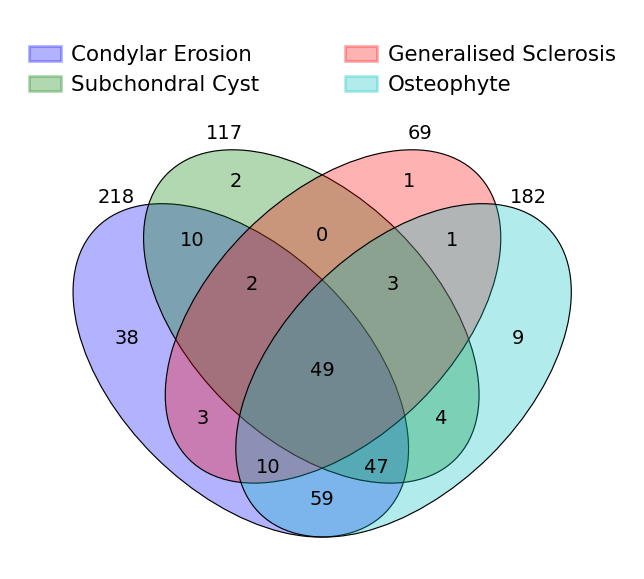
\includegraphics[width=0.5\textwidth]{figures/Venn.png}
  \caption{Four-set Venn diagram illustrating the co-occurrence of
  condylar erosion, generalised sclerosis, osteophyte, and subchondral
  cyst among the OA-positive joints in the full dataset.}
  \label{fig:venn}
\end{figure}

\subsubsection{Reference Standard and Inter-Rater Reliability}

Three oral and maxillofacial radiologists with 20--29~years of
experience independently labelled each joint for the five DC/TMD signs
(condylar erosion, generalised sclerosis, osteophyte, subchondral cyst,
and overall OA) using a standardised scoring sheet. The gold-standard
label for each sign was determined by majority vote. Inter-rater
reliability was quantified using Cohen's $\kappa$ for all pairwise
combinations and Fleiss' multi-rater $\kappa$
(Table~\ref{tab:irr}).

\begin{table}[htbp]
\centering
\caption{Inter-rater reliability statistics for four TMJOA radiographic
signs. Cohen's $\kappa$ is reported for each pairwise rater combination and
Fleiss' $\kappa$ reflects multi-rater
agreement.}
\label{tab:irr}
\small
\begin{tabular}{lcccc}
\toprule
\textbf{Sign} &
\textbf{$\kappa$ R1–R2} &
\textbf{$\kappa$ R1–R3} &
\textbf{$\kappa$ R2–R3} &
\textbf{Fleiss' $\kappa$} \\
\midrule
Osteoarthritis     & 0.847 & 0.869 & 0.892 & 0.869 \\
Erosion            & 0.810 & 0.852 & 0.871 & 0.844 \\
Generalised sclerosis & 0.557 & 0.630 & 0.864 & 0.664 \\
Osteophyte         & 0.780 & 0.803 & 0.932 & 0.837 \\
Subchondral cyst   & 0.670 & 0.629 & 0.645 & 0.648 \\
\bottomrule
\end{tabular}
\end{table}

\subsection{Preprocessing Pipeline}
\label{sec:preproc}

All volumes were preprocessed through a three-stage pipeline
(Figure~\ref{fig:preprocessing_pipeline}).

\begin{figure}[htbp]
  \centering
  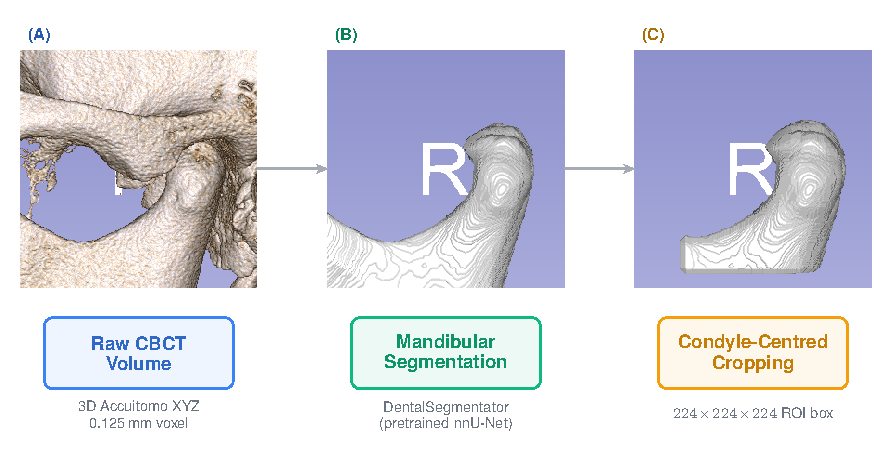
\includegraphics[width=0.9\textwidth]{figures/preprocess_pipeline.pdf}
  \caption{Preprocessing pipeline for condylar volume extraction. (A)~Raw CBCT volume acquired on a 3D Accuitomo XYZ scanner. (B)~Automatic mandibular segmentation using DentalSegmentator. (C)~Condyle-centred cropping via 3-D skeletonisation of the mandibular mask.}
  \label{fig:preprocessing_pipeline}
\end{figure}

\subsubsection{Stage 1: Mandibular Segmentation}

Automatic segmentation of the mandible was performed using
DentalSegmentator \cite{dot2024dentalsegmentator}, a publicly available
nnU-Net \cite{isensee2021nnu} model fine-tuned on a multi-centre dental
CBCT dataset. No further fine-tuning or manual correction was applied,
deliberately simulating real-world deployment conditions where post-hoc
mask editing is impractical. The segmentation mask was used exclusively
to define the bounding geometry of the mandible in subsequent steps.

\subsubsection{Stage 2: Condyle-Centred Cropping}

The condylar centre was identified via 3-D skeletonisation of the
mandibular mask using the \texttt{morphology.skeletonize} function from
scikit-image \cite{van2014scikit}. The skeleton was traversed to identify
the most superior branch tip, taken as a proxy for the condylar process
apex. A $224 \times 224 \times 224$~voxel region of interest was then
extracted, centred on this point.

\subsubsection{Stage 3: Intensity Normalisation}

Hounsfield unit values were windowed to the 2.5th–97.5th percentile range computed on the training dataset, encompassing soft-tissue and cortical bone intensities relevant to condylar morphology, then linearly rescaled to [0,1]. Processed volumes were saved in NIfTI format with all patient metadata stripped.

\subsection{Classification Framework}
\label{sec:framework}

\subsubsection{Task Definition}

For each condylar volume, the model predicted five independent binary labels corresponding to the DC/TMD signs: condylar erosion, generalised sclerosis, osteophyte, subchondral cyst, and overall OA.

\subsubsection{Classification Models}

Twenty backbone architectures spanning CNNs, lightweight mobile
networks, vision transformers, and hybrid designs were evaluated. All
backbones were initialised from ImageNet pre-trained weights; when
multiple weight sets existed for a given variant, the one with the
highest ImageNet top-1 accuracy was selected, and the largest publicly
available variant of each architecture was used to maximise
representational capacity. The specific variant and weight configuration
for each architecture are listed in Supplementary Table S1.
Weights were sourced from the TorchVision
library \cite{torchvision} for all architectures except YOLOv11x-cls,
which used Ultralytics \cite{yolo11_ultralytics}. All backbone parameters were frozen during training; only the classification heads were updated, reducing the risk of overfitting on the limited training set. For each
backbone, the original classification layer was replaced with five
task-specific multi-layer perceptron heads ($512 \to 256 \to 1$ with
ReLU activations and dropout $p = 0.3$), attached to the pooled feature
representation (Figure~\ref{fig:model_architecture}).

\begin{figure}[htbp]
  \centering
  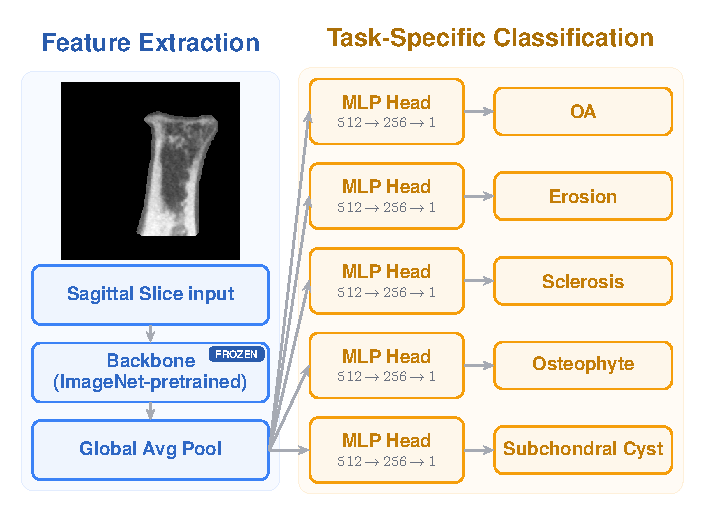
\includegraphics[width=0.65\textwidth]{figures/architecture_pipeline.pdf}
  \caption{Classification framework architecture. Left: the feature
  extraction pipeline consisting of a sagittal slice input, a frozen
  ImageNet-pretrained backbone, and global average pooling. Right: five
  task-specific MLP heads ($512 \to 256 \to 1$ with ReLU and dropout
  $p = 0.3$), one per DC/TMD sign.}
  \label{fig:model_architecture}
\end{figure}

\subsubsection{Loss Function and Optimisation}

Binary cross-entropy with logits (\texttt{BCEWithLogitsLoss}) was used
for all tasks. Minority-class oversampling was applied for generalised
sclerosis and subchondral cyst to address class imbalance. All models
were optimised with stochastic gradient descent (SGD) with cosine
annealing of the learning rate.

\subsubsection{Two-Stage Training Strategy}

To leverage the coarse-to-fine relationship among labels (OA is positive
whenever any other sign is present), a two-stage training strategy was
adopted. In Stage~1, the classification head was trained for OA
classification. In Stage~2, the OA-trained head weights initialised the
four sign-specific heads (condylar erosion, generalised sclerosis,
osteophyte, subchondral cyst), which were then fine-tuned independently.

\subsubsection{Data Augmentation}

Online data augmentation was applied to each sampled training slice
using a RandAugment-style policy \cite{cubuk2020randaugment}. A pool of
17 candidate transformations (10 intensity, 6 spatial and an identity transformation) was assembled
from the MONAI library \cite{monai2026}. For each training sample, two
transformations were drawn uniformly at random from this pool, transformation magnitude was then randomised
within the admissible range. No augmentation was applied during
validation or testing. The full transformation list and admissible
parameter ranges are provided in Supplementary
Table S3.

\subsubsection{Threshold Selection}
\label{sec:threshold_selection}
For each task, the classification threshold was set at
the value maximising Youden's $J$ statistic
($J = \text{sensitivity} + \text{specificity} - 1$) on the validation set.

\subsection{Informativeness-Weighted 2-D Slice Sampling}

Each 3-D volume was treated as a pool of 2-D sagittal slices. An
\emph{informativeness score} was defined for each slice as the ratio of
the number of pixels belonging to the segmented condylar region to the
total number of pixels in the slice:
\begin{equation}
  s_i = \frac{\text{Segmented condylar pixels in slice } i}
             {\text{Total pixels in slice } i}.
  \label{eq:info}
\end{equation}

\subsubsection{Slice sampling during training}

During training, a single slice was sampled from each volume in the training batch with probability proportional to~$s_i$, encouraging the model
to learn from slices rich in condylar anatomy
(Figure~\ref{fig:training_pipeline}). Grayscale slices were replicated
to three channels to match ImageNet-pretrained backbone input
requirements.

\begin{figure}[htbp]
  \centering
  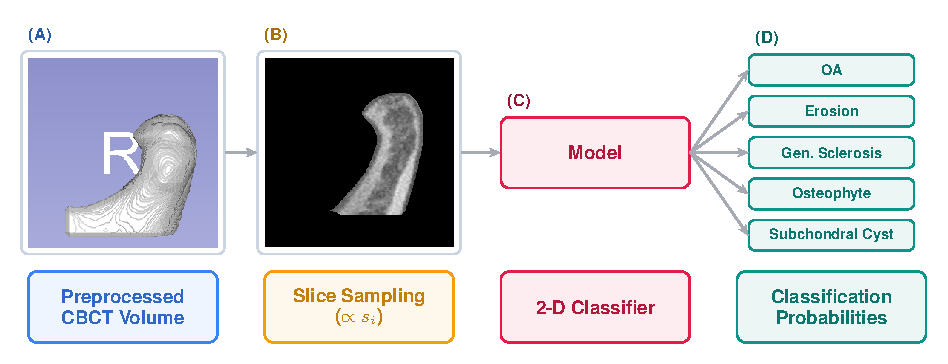
\includegraphics[width=0.9\textwidth]{figures/train_pipeline.pdf}
  \caption{Inference process during training. (A)~Preprocessed CBCT volume input. (B)~A single sagittal slice is sampled with probability proportional to its informativeness score~$s_i$. (C)~The sampled slice is passed through the model. (D)~Five independent binary classification outputs.}
  \label{fig:training_pipeline}
\end{figure}

\subsubsection{Slice aggregation during deployment.}

In deployment, all sagittal slices with an informativeness score
$s_i > 0.05$ were filtered to exclude peripheral slices containing
negligible condylar anatomy. To reduce redundancy among visually similar
consecutive slices, every third slice from this filtered subset was
retained. Slice-level predictions from the resulting set were combined
into a volume-level probability using an informativeness-weighted average
(Figure~\ref{fig:inference_pipeline}):
\begin{equation}
  \hat{p} = \frac{\sum_{j \in \mathcal{J}} s_j \cdot \sigma(\hat{y}_j)}
                 {\sum_{j \in \mathcal{J}} s_j},
  \label{eq:agg}
\end{equation}
where $\mathcal{J}$ denotes the index set of retained slices, $\sigma(\cdot)$ is
the sigmoid function, and $\hat{y}_j$ is the logit for slice~$j$.
The volume-level probability~$\hat{p}$ was then compared against the task-specific threshold selected on the validation set
(Section~\ref{sec:threshold_selection}) to produce the final binary prediction.
The test results reported in Section~\ref{sec:results} were obtained using this inference procedure.

\begin{figure}[htbp]
  \centering
  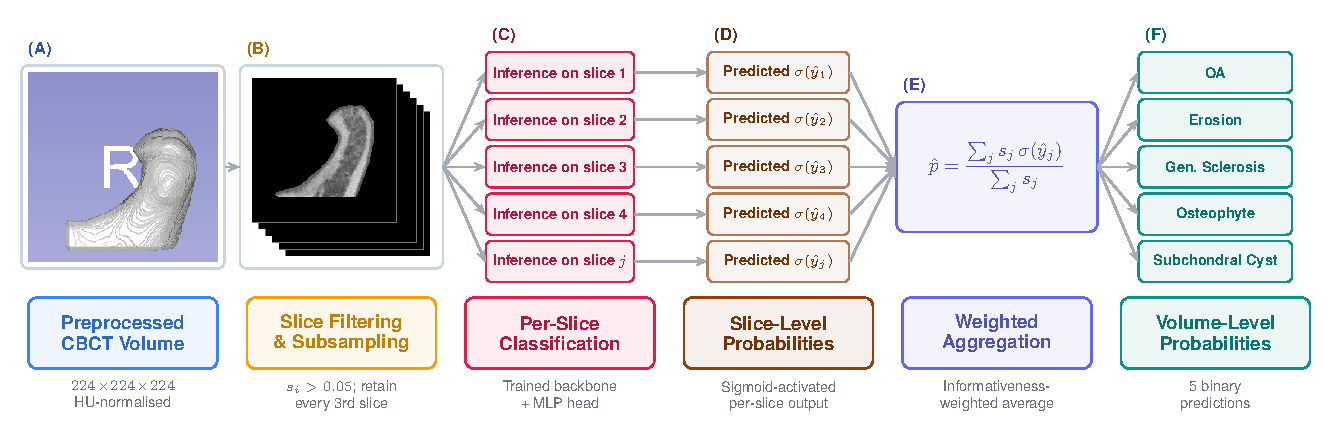
\includegraphics[width=\textwidth]{figures/inference_pipeline.pdf}
  \caption{Inference process in deployment. (A)~Preprocessed CBCT volume input. (B)~Sagittal slices are filtered and subsampled. (C)~Each retained slice is independently classified by the trained model. (D)~Slice-level sigmoid probabilities output $\sigma(\hat{y}_j)$. (E)~Informativeness-weighted aggregation produces volume-level probability $\hat{p}$ (Equation~\ref{eq:agg}). (F)~Final binary predictions.}
  \label{fig:inference_pipeline}
\end{figure}

\subsection{Explainability}
\label{sec:xai}

GradCAM \cite{Selvaraju_2019} was applied to all models at inference.
The resulting activation maps were overlaid on the corresponding
sagittal slices for visual inspection.
Qualitative results are reported for the highest-ranked model
(ConvNeXt) (Figure~\ref{fig:gradcam}).

\subsection{Evaluation Metrics}
\label{sec:metrics}

Performance was evaluated on the held-out test set (43~joints) using
accuracy, precision, recall, F1 score, area under the
receiver-operating characteristic curve (AUC-ROC) and area under the precision-recall curve (AUC-PR). Emphasis is placed
on AUC-ROC and AUC-PR as threshold-independent metrics.

\subsection{Implementation Details}
\label{sec:impl}

All models were implemented in Python using PyTorch~2.9.0
\cite{paszke2019pytorch}, the Ultralytics library~8.4.14
\cite{yolo11_ultralytics} (for YOLOv11), and MONAI~1.5.2
\cite{monai2026} for volumetric data handling. 
Visual inspection of raw CBCT volumes and preprocessed outputs at each pipeline stage was performed using 3D Slicer~5.8.1 \cite{fedorov20123d}.
Training was performed on
an NVIDIA~L4 GPU; each model--task combination required approximately
2--3~hours. All models were trained with an initial learning rate of
$10^{-2}$, cosine annealing, and a batch size of~8 for 1000~epochs per
task, with early stopping triggered after 50 consecutive epochs without
validation loss improvement. Because slice sampling is stochastic,
validation was performed three times per epoch and the scores averaged.

\subsection{Native 3-D Baseline: MONAI ResNet50}
\label{sec:monai3d}

To contextualise the 2-D slice sampling approach, a native 3-D ResNet50
baseline was trained directly on the preprocessed CBCT volumes using the MONAI framework \cite{monai2026}. This model processes the entire volumetric input in a single forward pass without
any dimensionality reduction or slice sampling, representing the most
straightforward application of a deep learning classifier to 3D CBCT image. The architecture followed the standard ResNet50 design with 3D
convolutional kernels throughout, initialised with random weights. The same
two-stage training strategy, loss function, classifier head, and
SGD optimiser with cosine annealing were applied for consistency;
batch size was set to~2 owing to GPU memory constraints imposed by the
full volumetric input.

%% ===================================================================
\section{Results}
\label{sec:results}
%% ===================================================================

\subsection{Inter-Rater Reliability and Rater Performance}
\label{sec:irr_results}

Inter-rater reliability statistics are presented in
Table~\ref{tab:irr}. Agreement was excellent for erosion
(Fleiss' $\kappa = 0.844$) and osteophyte ($\kappa = 0.837$), and
moderate for generalised sclerosis ($\kappa = 0.664$) and subchondral
cyst ($\kappa = 0.648$).

\subsection{Model Performance}
\label{sec:model_results}
 
Per-task AUC-ROC and AUC-PR for each architecture is reported in
Table~\ref{tab:model_summary}. Full results including
accuracy, precision, recall, and F1 are provided in Supplementary
Table S2.

\begin{table}[htbp]
\centering
\caption{Test-set AUC-ROC and AUC-PR for all 20 architectures across five tasks,
sorted by mean AUC-ROC. Best value per sub-column in \textbf{bold}.}
\label{tab:model_summary}
\small
\setlength{\tabcolsep}{2.5pt}
\begin{tabular}{l cc cc cc cc cc cc}
\toprule
& \multicolumn{2}{c}{\textbf{OA}}
& \multicolumn{2}{c}{\textbf{Erosion}}
& \multicolumn{2}{c}{\textbf{Sclerosis}}
& \multicolumn{2}{c}{\textbf{Osteophyte}}
& \multicolumn{2}{c}{\textbf{Cyst}}
& \multicolumn{2}{c}{\textbf{Mean}} \\
\cmidrule(lr){2-3}\cmidrule(lr){4-5}\cmidrule(lr){6-7}\cmidrule(lr){8-9}\cmidrule(lr){10-11}\cmidrule(lr){12-13}
\textbf{Model}
& \textit{ROC} & \textit{PR}
& \textit{ROC} & \textit{PR}
& \textit{ROC} & \textit{PR}
& \textit{ROC} & \textit{PR}
& \textit{ROC} & \textit{PR}
& \textit{ROC} & \textit{PR} \\
\midrule
ConvNeXt            & \textbf{.991} & \textbf{.994} & \textbf{.952} & \textbf{.941} & .944 & .595 & .921 & .803 & .823 & .528 & \textbf{.926} & .772 \\
DenseNet            & .987 & .992 & .945 & .926 & .913 & .593 & .923 & .908 & .836 & .588 & .921 & .801 \\
ViT                 & .980 & .986 & .939 & .927 & .893 & .543 & \textbf{.950} & \textbf{.942} & .841 & .627 & .920 & .805 \\
Inception V3        & .978 & .986 & .936 & .931 & .909 & .589 & .925 & .892 & \textbf{.849} & \textbf{.678} & .919 & .815 \\
ResNeXt             & .984 & .989 & .943 & .929 & .909 & .460 & .921 & .839 & .839 & .584 & .919 & .760 \\
Swin Transformer    & .964 & .976 & .925 & .925 & \textbf{.956} & .719 & .917 & .869 & .828 & .554 & .918 & .809 \\
YOLOv11             & .980 & .987 & .939 & .932 & .917 & \textbf{.768} & .906 & .877 & .844 & .643 & .917 & .841 \\
VGG                 & .971 & .981 & .923 & .916 & .937 & .569 & .917 & .904 & .828 & .626 & .915 & .799 \\
Swin Transformer V2 & .969 & .979 & .923 & .902 & .925 & .504 & .921 & .891 & .836 & .598 & .915 & .775 \\
RegNetX             & .978 & .985 & .939 & .931 & .921 & .741 & .925 & .897 & .808 & .672 & .914 & \textbf{.845} \\
MobileNet V2        & .976 & .985 & .925 & .879 & .929 & .548 & .904 & .847 & .833 & .560 & .913 & .764 \\
GoogLeNet           & .976 & .983 & .930 & .925 & .929 & .534 & .906 & .869 & .823 & .533 & .913 & .769 \\
MobileNet V3        & .984 & .989 & .945 & .917 & .893 & .582 & .919 & .802 & .808 & .513 & .910 & .760 \\
EfficientNet V2     & .969 & .979 & .925 & .918 & .901 & .452 & .923 & .905 & .826 & .562 & .909 & .763 \\
MaxViT              & .971 & .981 & .921 & .874 & .877 & .423 & .941 & .933 & .821 & .517 & .906 & .746 \\
ShuffleNet V2       & .960 & .974 & .912 & .910 & .921 & .677 & .921 & .915 & .780 & .504 & .899 & .796 \\
EfficientNet        & .969 & .979 & .910 & .837 & .885 & .436 & .936 & .921 & .782 & .542 & .896 & .743 \\
ResNet              & .980 & .986 & .932 & .881 & .821 & .470 & .932 & .916 & .805 & .649 & .894 & .780 \\
MNASNet             & .951 & .966 & .930 & .916 & .893 & .647 & .886 & .767 & .800 & .624 & .892 & .784 \\
RegNetY             & .951 & .970 & .908 & .867 & .837 & .364 & .893 & .862 & .767 & .542 & .871 & .721 \\
\midrule
\textbf{Mean}       & .973 & .982 & .930 & .909 & .905 & .561 & .919 & .878 & .819 & .582 & .909 & .782 \\
\bottomrule
\end{tabular}
\end{table}

Best model by observed mean AUC-ROC, ConvNeXt achieved near-perfect discrimination for OA
(AUC-ROC 0.991) and strong performance on erosion (0.952), generalised
sclerosis (0.944), and osteophyte (0.921), with lower performance on
the imbalanced subchondral cyst class (0.823).
 
Bootstrap resampling (10{,}000 iterations, Holm--Bonferroni correction
over 190 pairwise tests, $\alpha = 0.05$) revealed no statistically
significant pairwise differences in mean AUC-ROC, likely owing to the
limited test-set size ($n = 43$). ConvNeXt achieved the highest
observed mean AUC-ROC (0.926) and ranked first most frequently (28.5\%
of resamples; mean rank 3.4), followed by DenseNet201 (0.921; mean rank
5.5) and ViT-L/16 (0.920; mean rank 5.8), although substantial rank
overlap among the top 10 architectures indicates that these differences
are not robust to sampling variability
(Figure~\ref{fig:bootstrap_rank}). Notably, vision transformers
performed comparably to lightweight CNNs such as MobileNet~V2 (0.914),
indicating that ImageNet-pretrained CNN features transfer effectively to
this domain even without architectural complexity.

\begin{figure}[htbp]
  \centering
  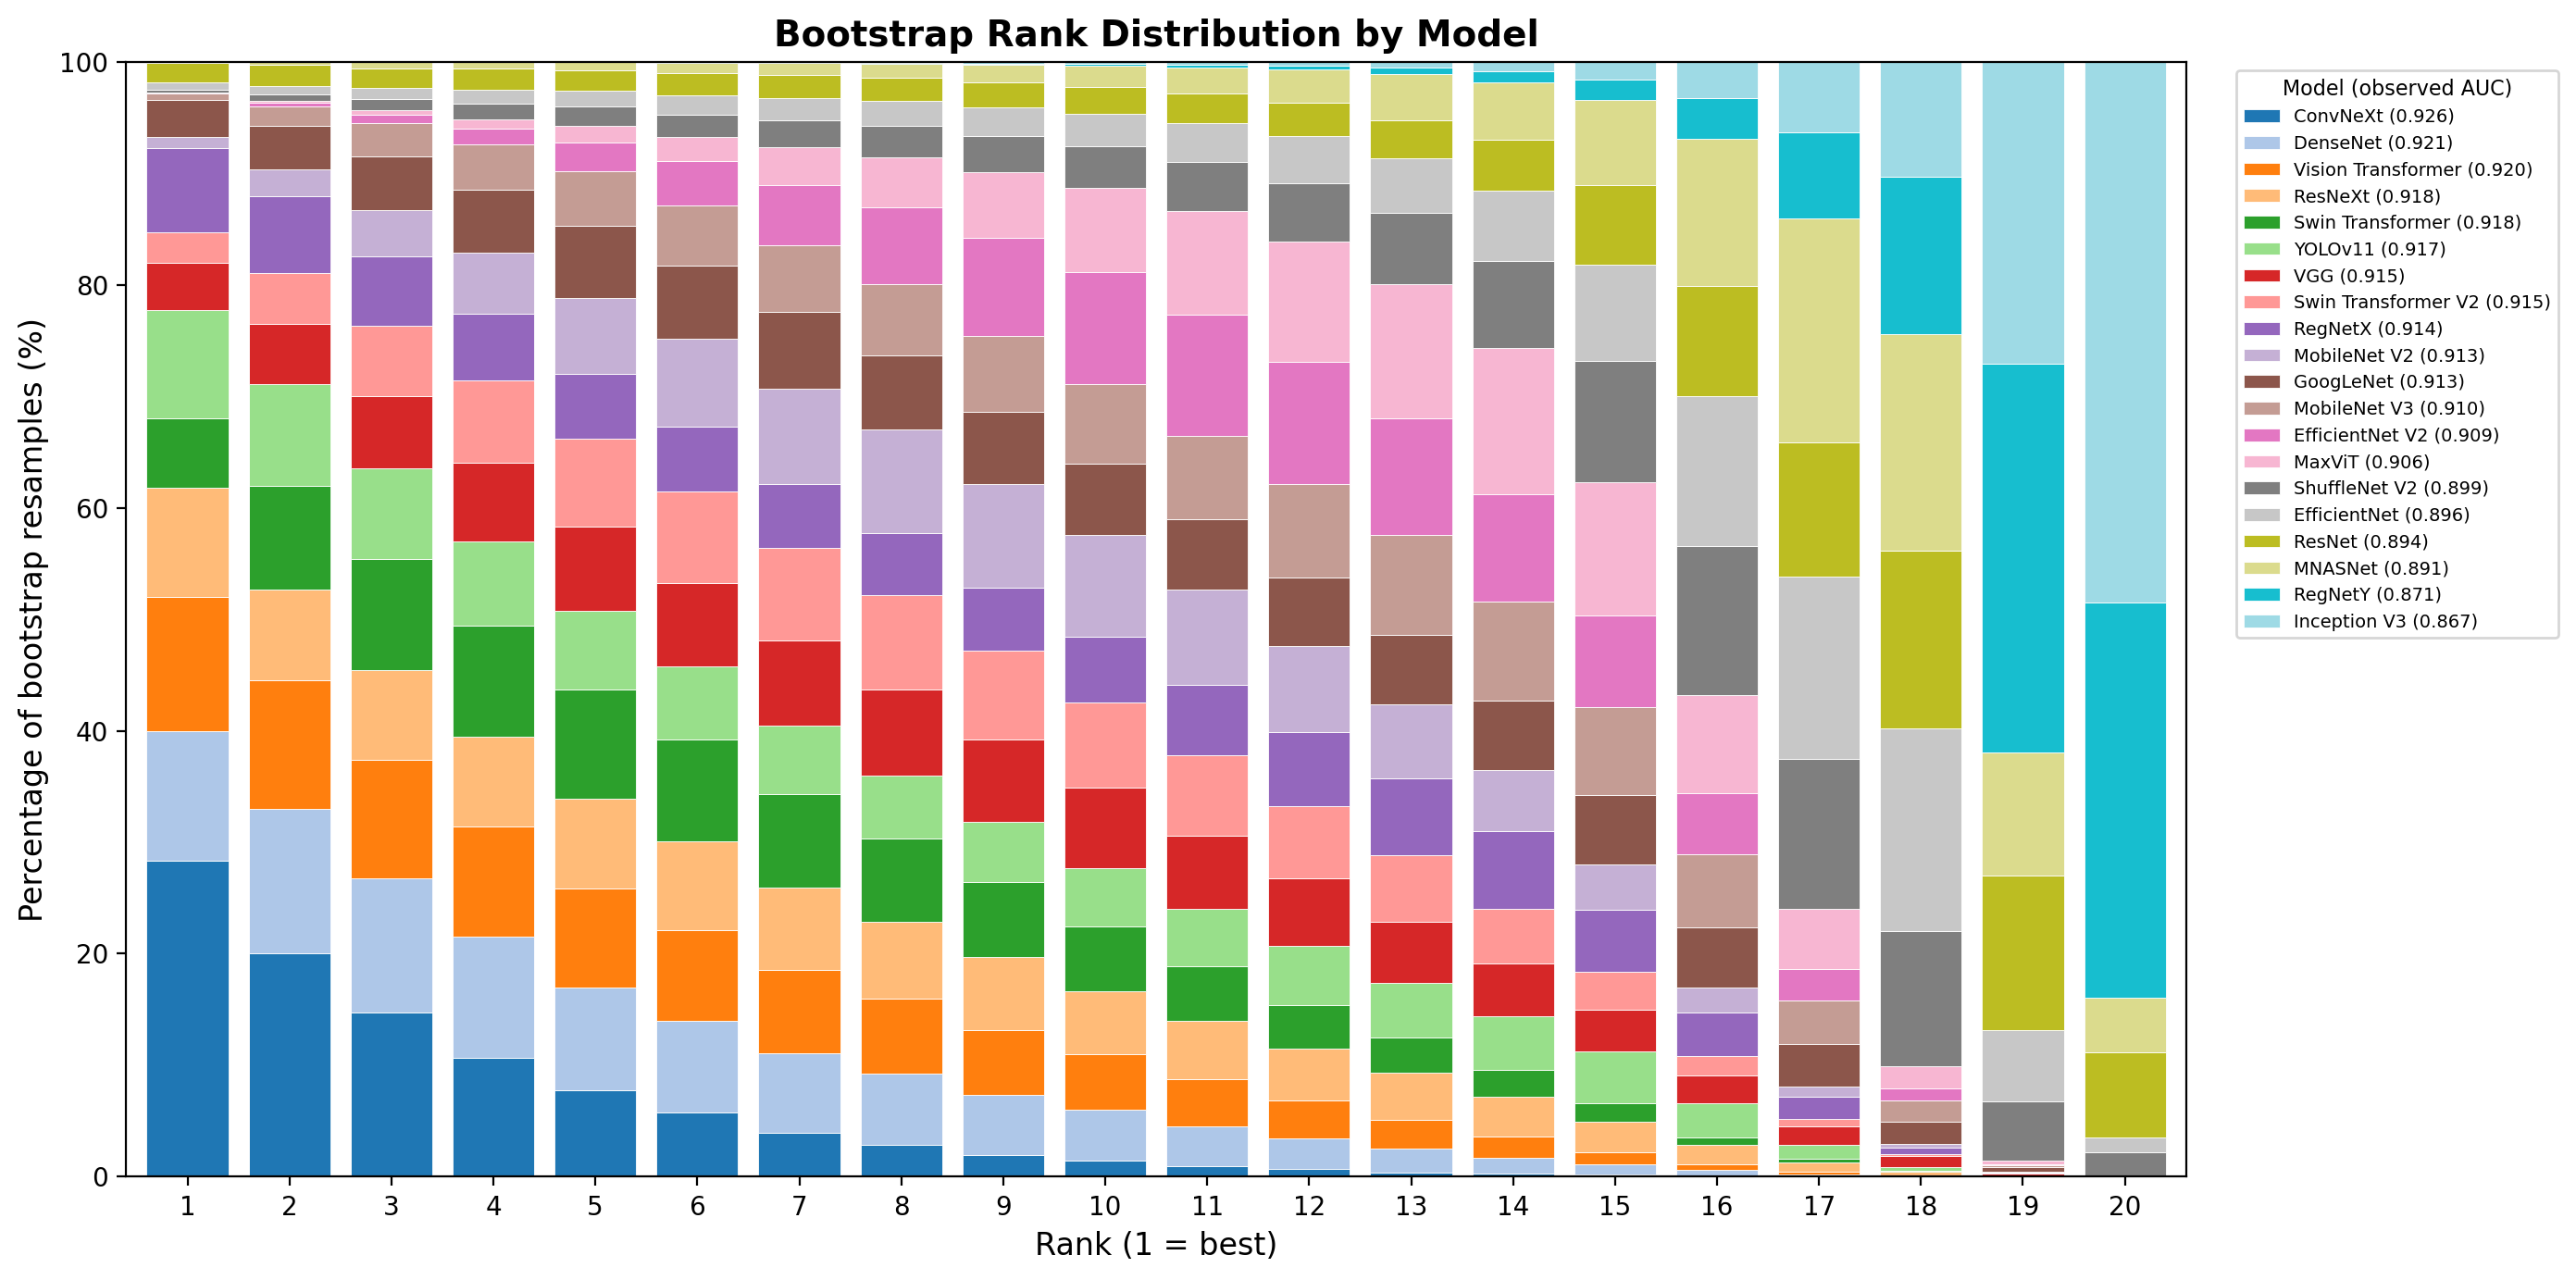
\includegraphics[width=0.8\textwidth]{figures/bootstrap_dist.png}
  \caption{Bootstrap rank distribution across 10{,}000 resamples for all
  20 architectures, sorted by observed mean AUC-ROC. Stacked bars indicate the
  proportion of resamples in which each architecture achieved a given
  rank. Substantial rank overlap among the top 10 models indicates that
  observed performance differences are not robust to sampling
  variability.}
  \label{fig:bootstrap_rank}
\end{figure}



\subsection{Task-Level Summary}
\label{sec:task_summary}

As shown in the mean row of Table~\ref{tab:model_summary}, OA achieved
the highest mean AUC-ROC (0.973), followed by erosion (0.930),
osteophyte (0.919), generalised sclerosis (0.905), and subchondral cyst
(0.819). Although generalised sclerosis and subchondral cyst achieved
comparable AUC-ROC values, their mean AUC-PR scores (0.561 and 0.582,
respectively) were substantially lower than
those of the other tasks, reflecting the combined effect of class
imbalance and moderate inter-rater reliability.

\subsection{Explainability}
\label{sec:xai_results}

GradCAM visualisations for ConvNeXt (Figure~\ref{fig:gradcam}) showed
activation concentrated on anatomically relevant condylar regions across
all five tasks, confirming that predictions were driven by meaningful
morphological features rather than background artefacts. The activation
pattern for subchondral cyst closely resembled that of the overall OA
task, suggesting that this sign-specific head may not have learned
features beyond those acquired during OA initialisation, a likely consequence of the two-stage
training strategy.

\begin{figure}[htbp]
  \centering
  \newlength{\cellw}
  \setlength{\cellw}{0.25\textwidth}
  \newcolumntype{L}{>{\raggedright\arraybackslash}p{\cellw}}
  \begin{tabular}{@{}LLL@{}}
    \textbf{(A)} & \textbf{(B)} & \textbf{(C)} \\[-2pt]
    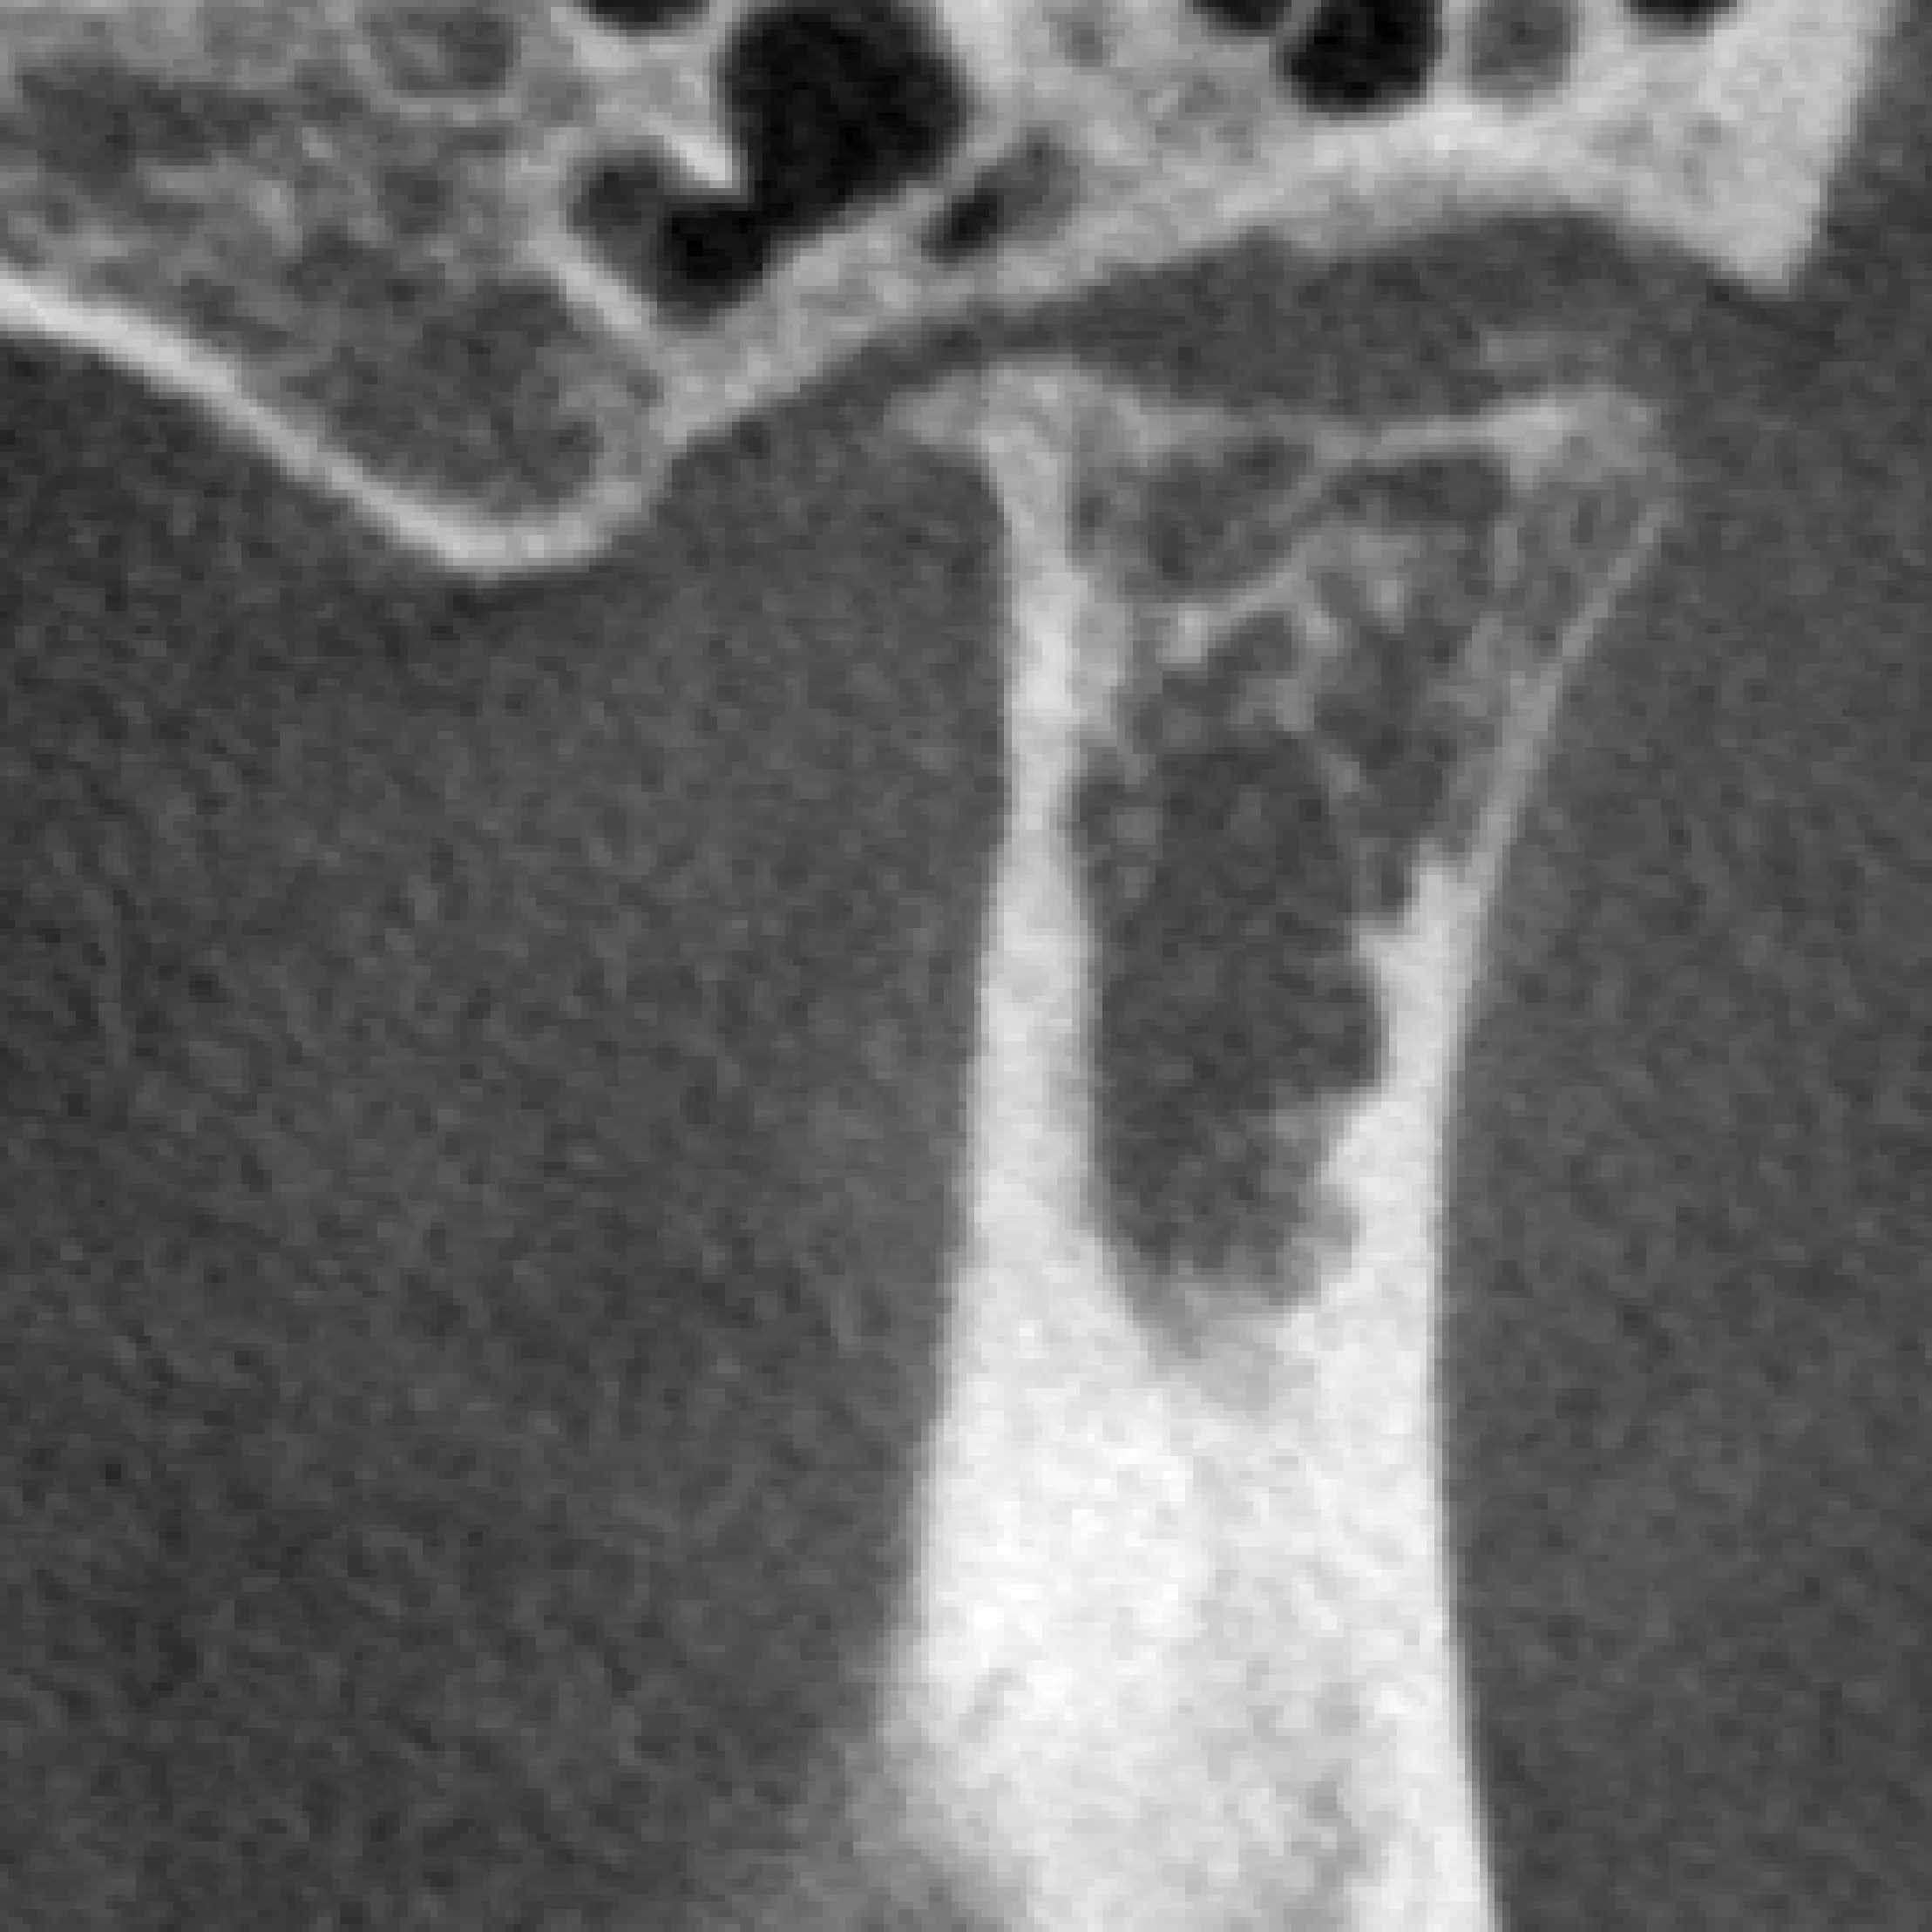
\includegraphics[width=0.81\cellw]{figures/original_130.png} &
    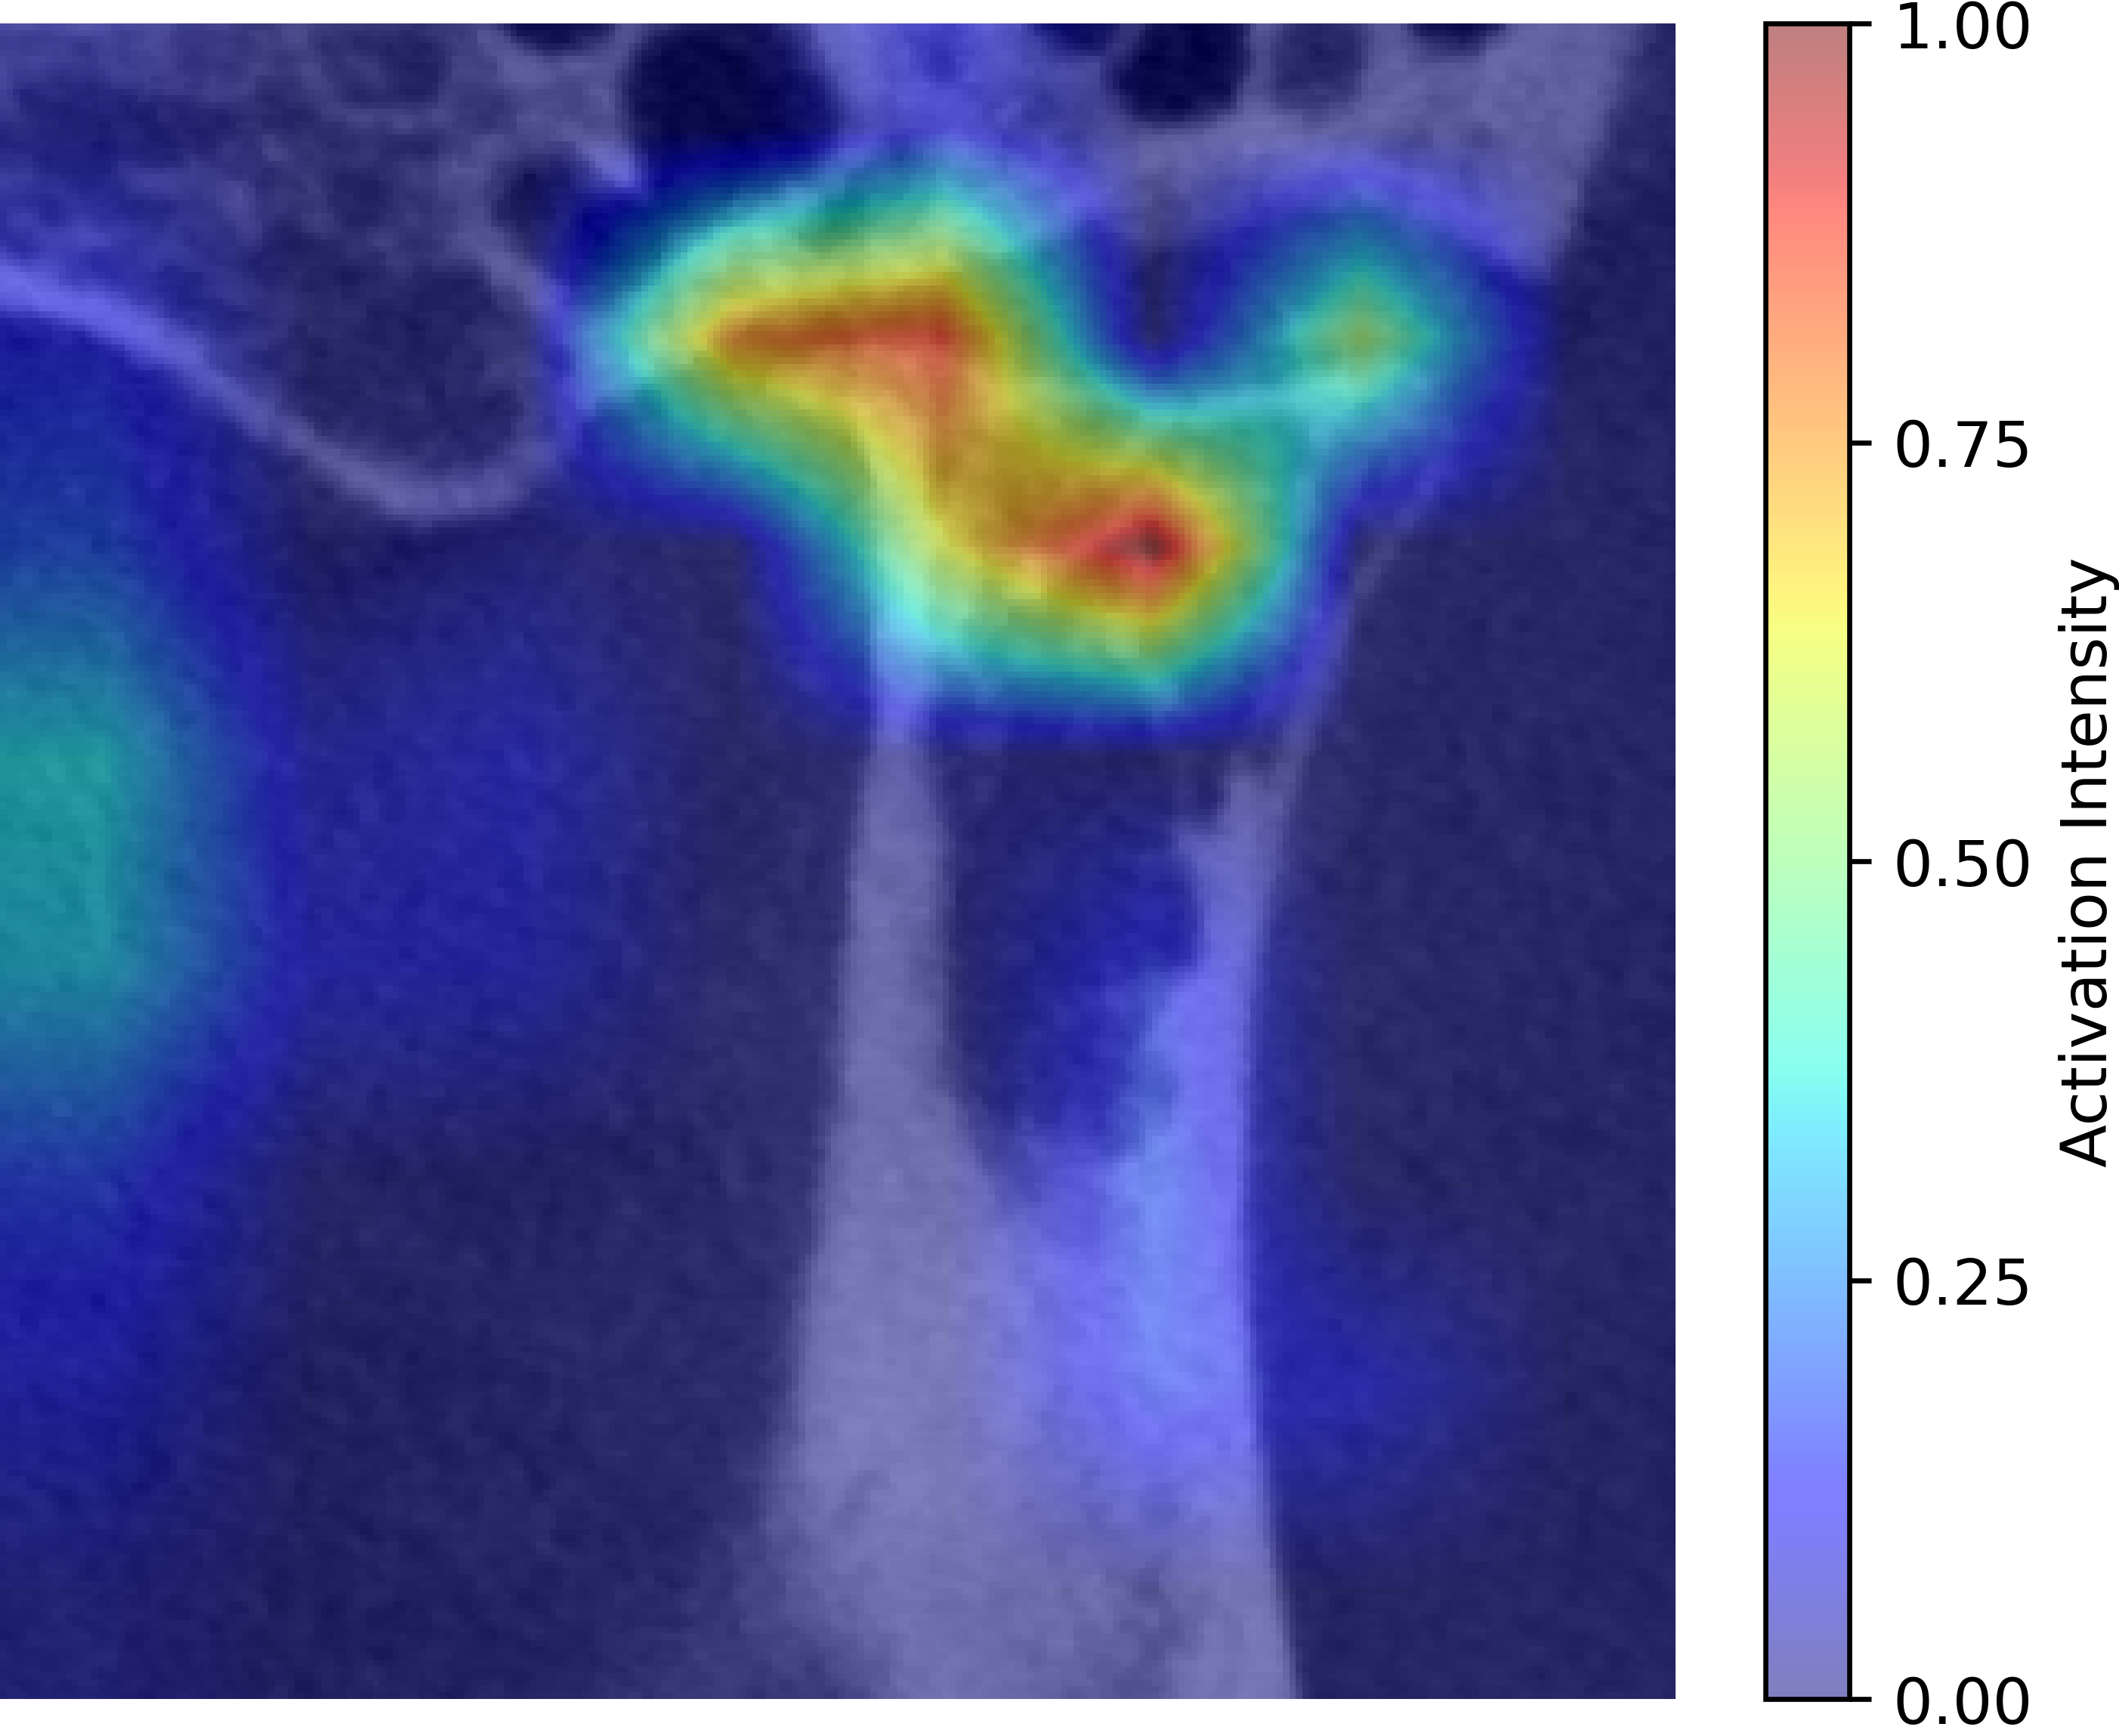
\includegraphics[width=\cellw]{figures/OA_overlayed_130.png} &
    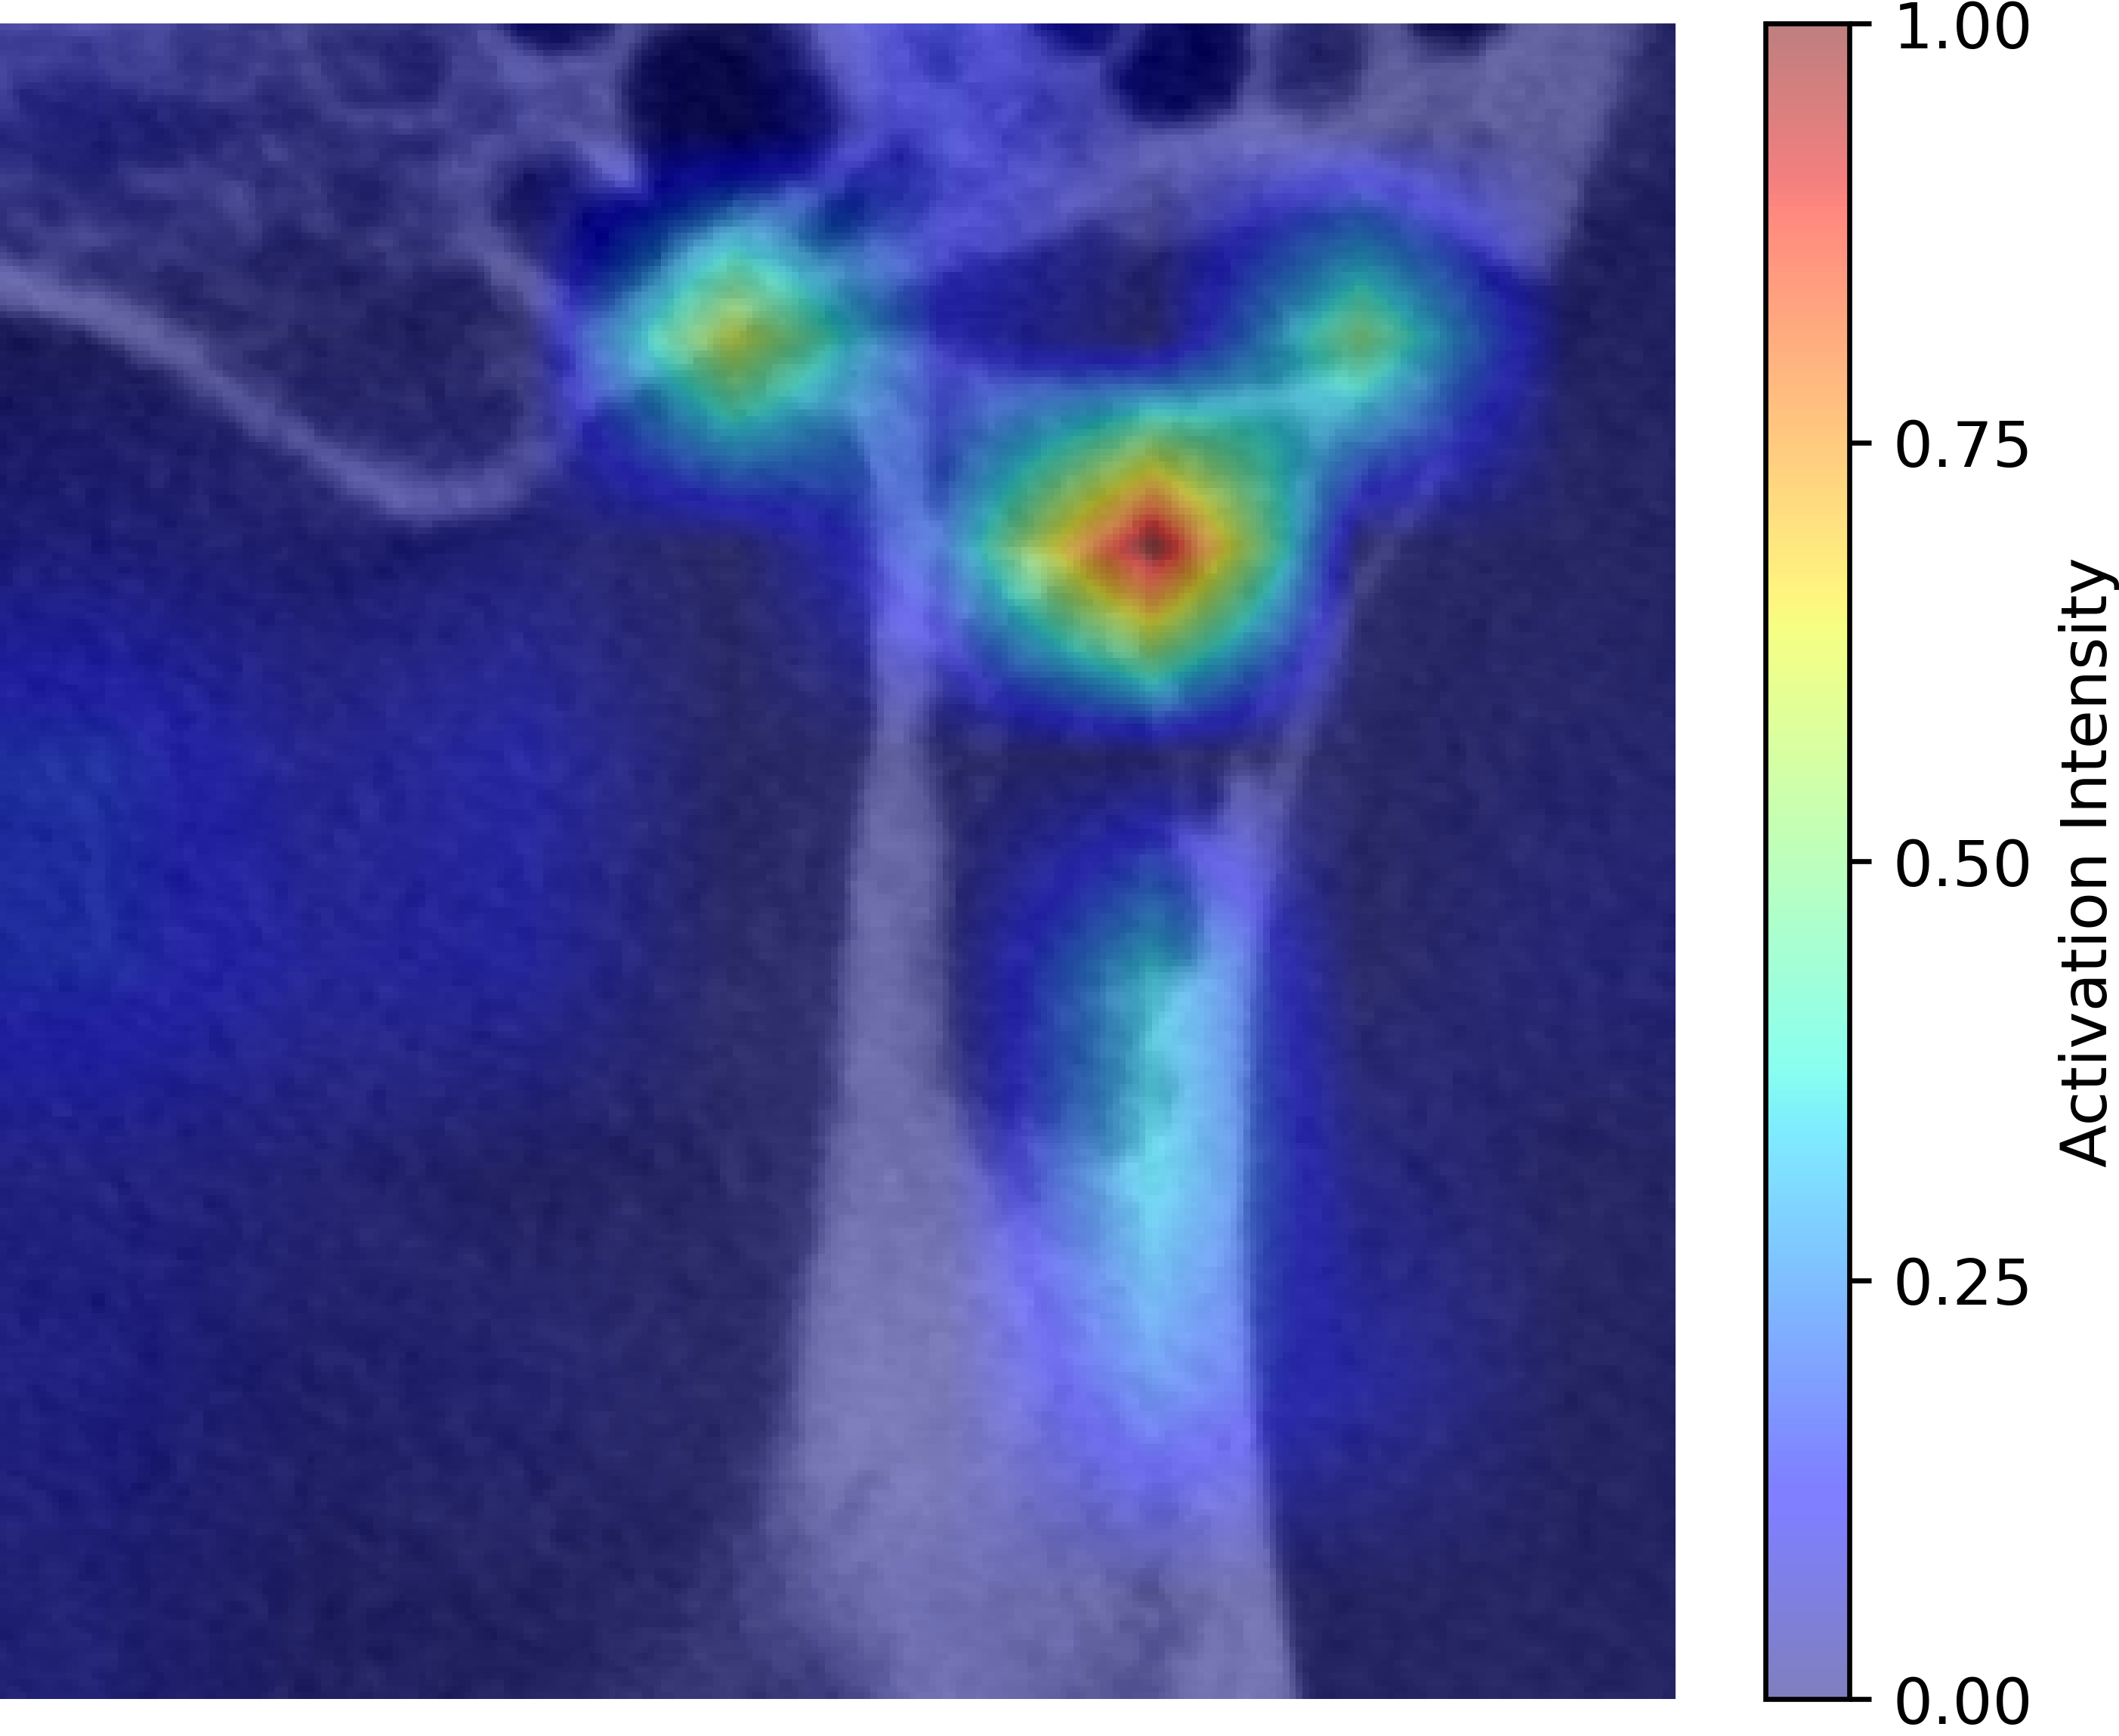
\includegraphics[width=\cellw]{figures/erosion_overlayed_130.png} \\[6pt]
    \textbf{(D)} & \textbf{(E)} & \textbf{(F)} \\[-2pt]
    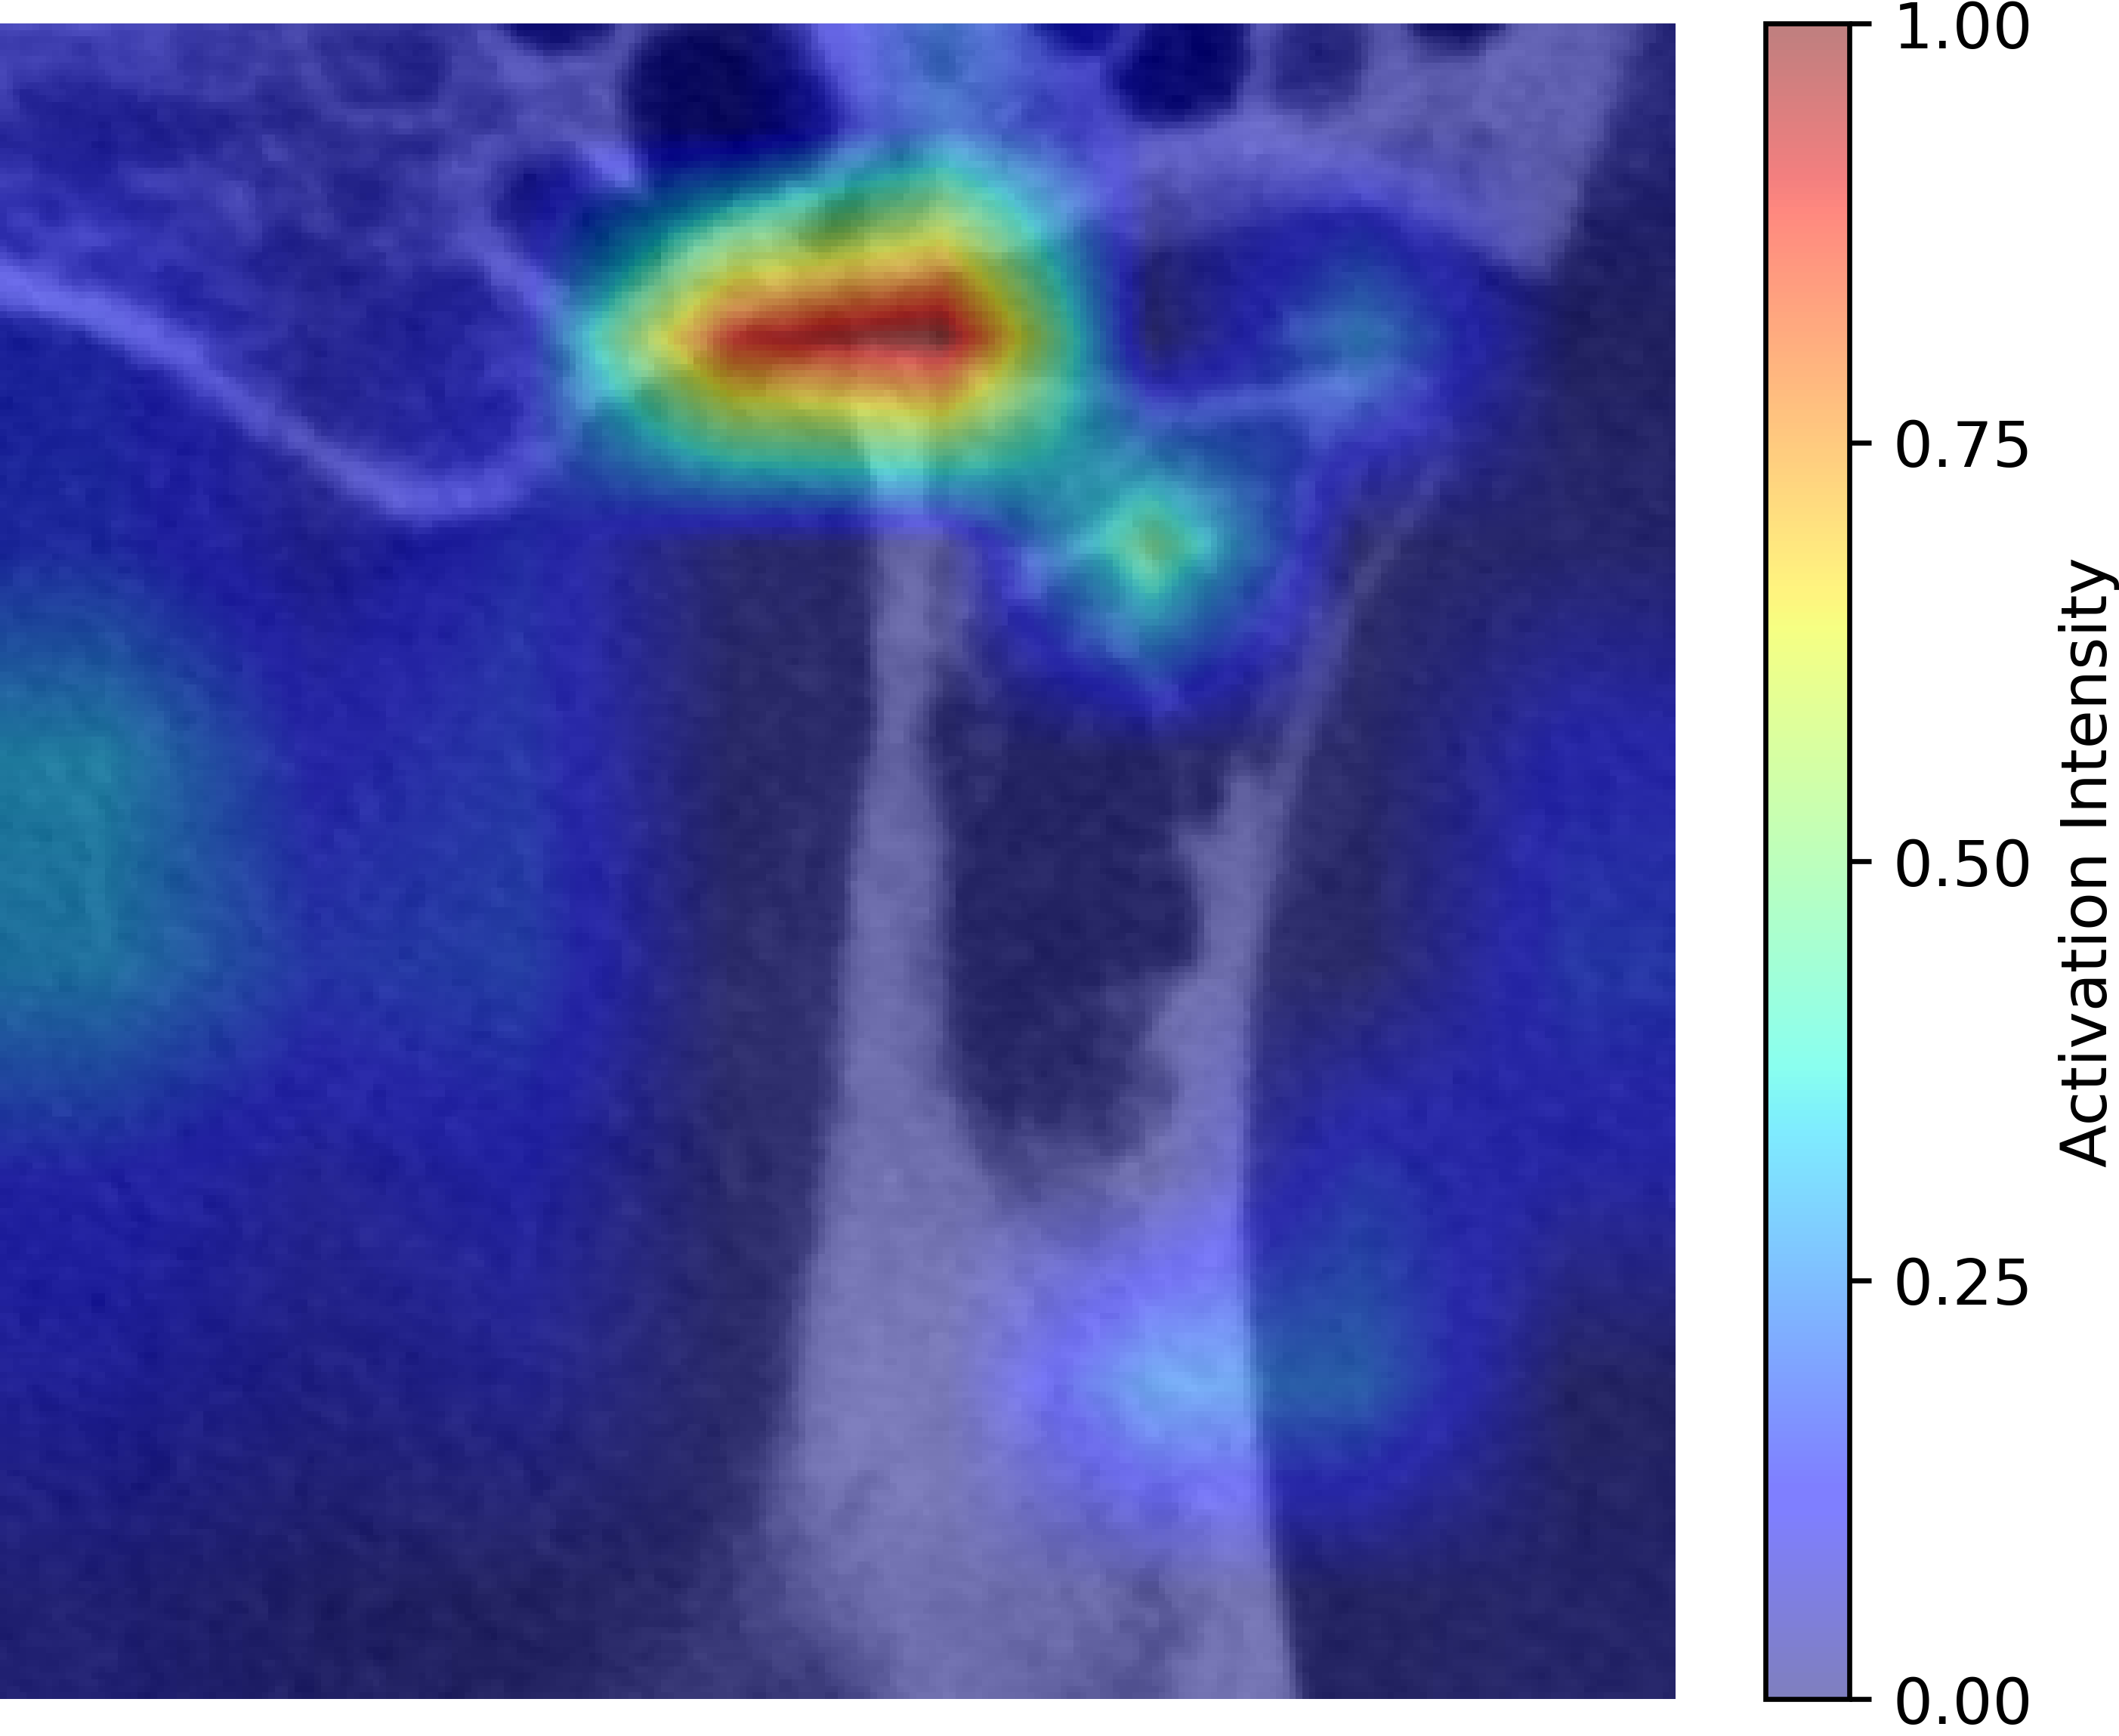
\includegraphics[width=\cellw]{figures/genSclerosis_overlayed_130.png} &
    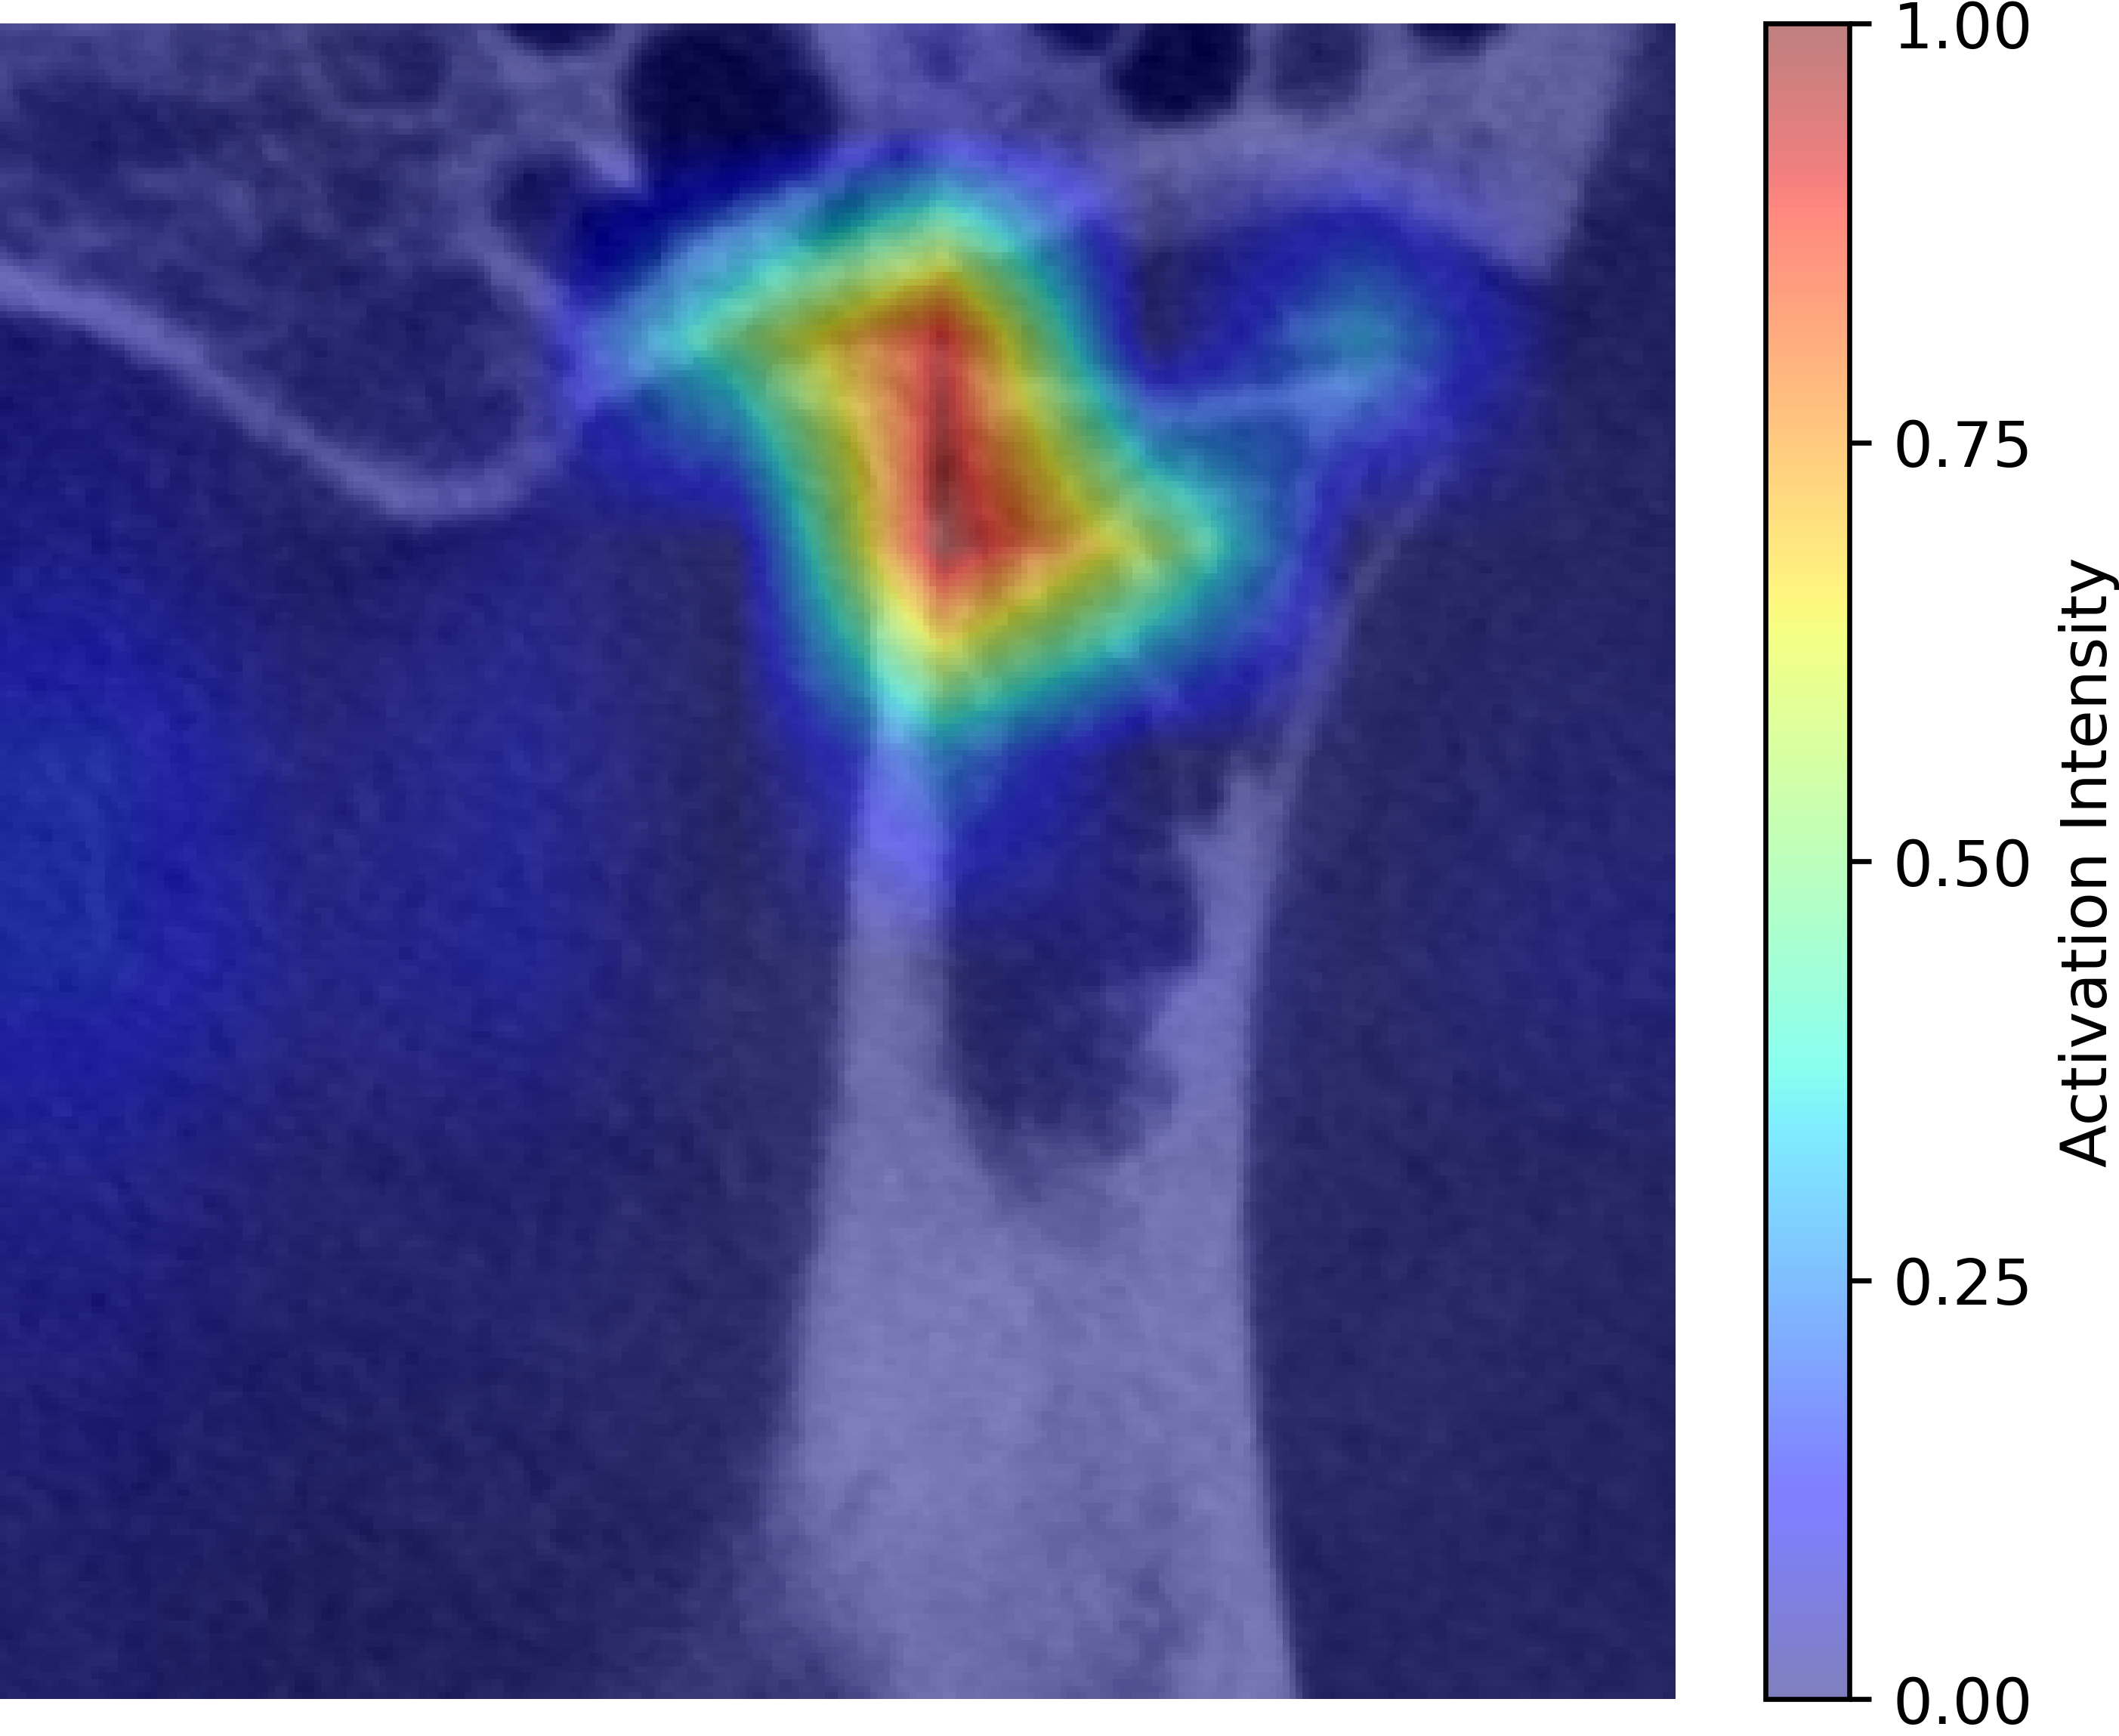
\includegraphics[width=\cellw]{figures/osteophyte_overlayed_130.png} &
    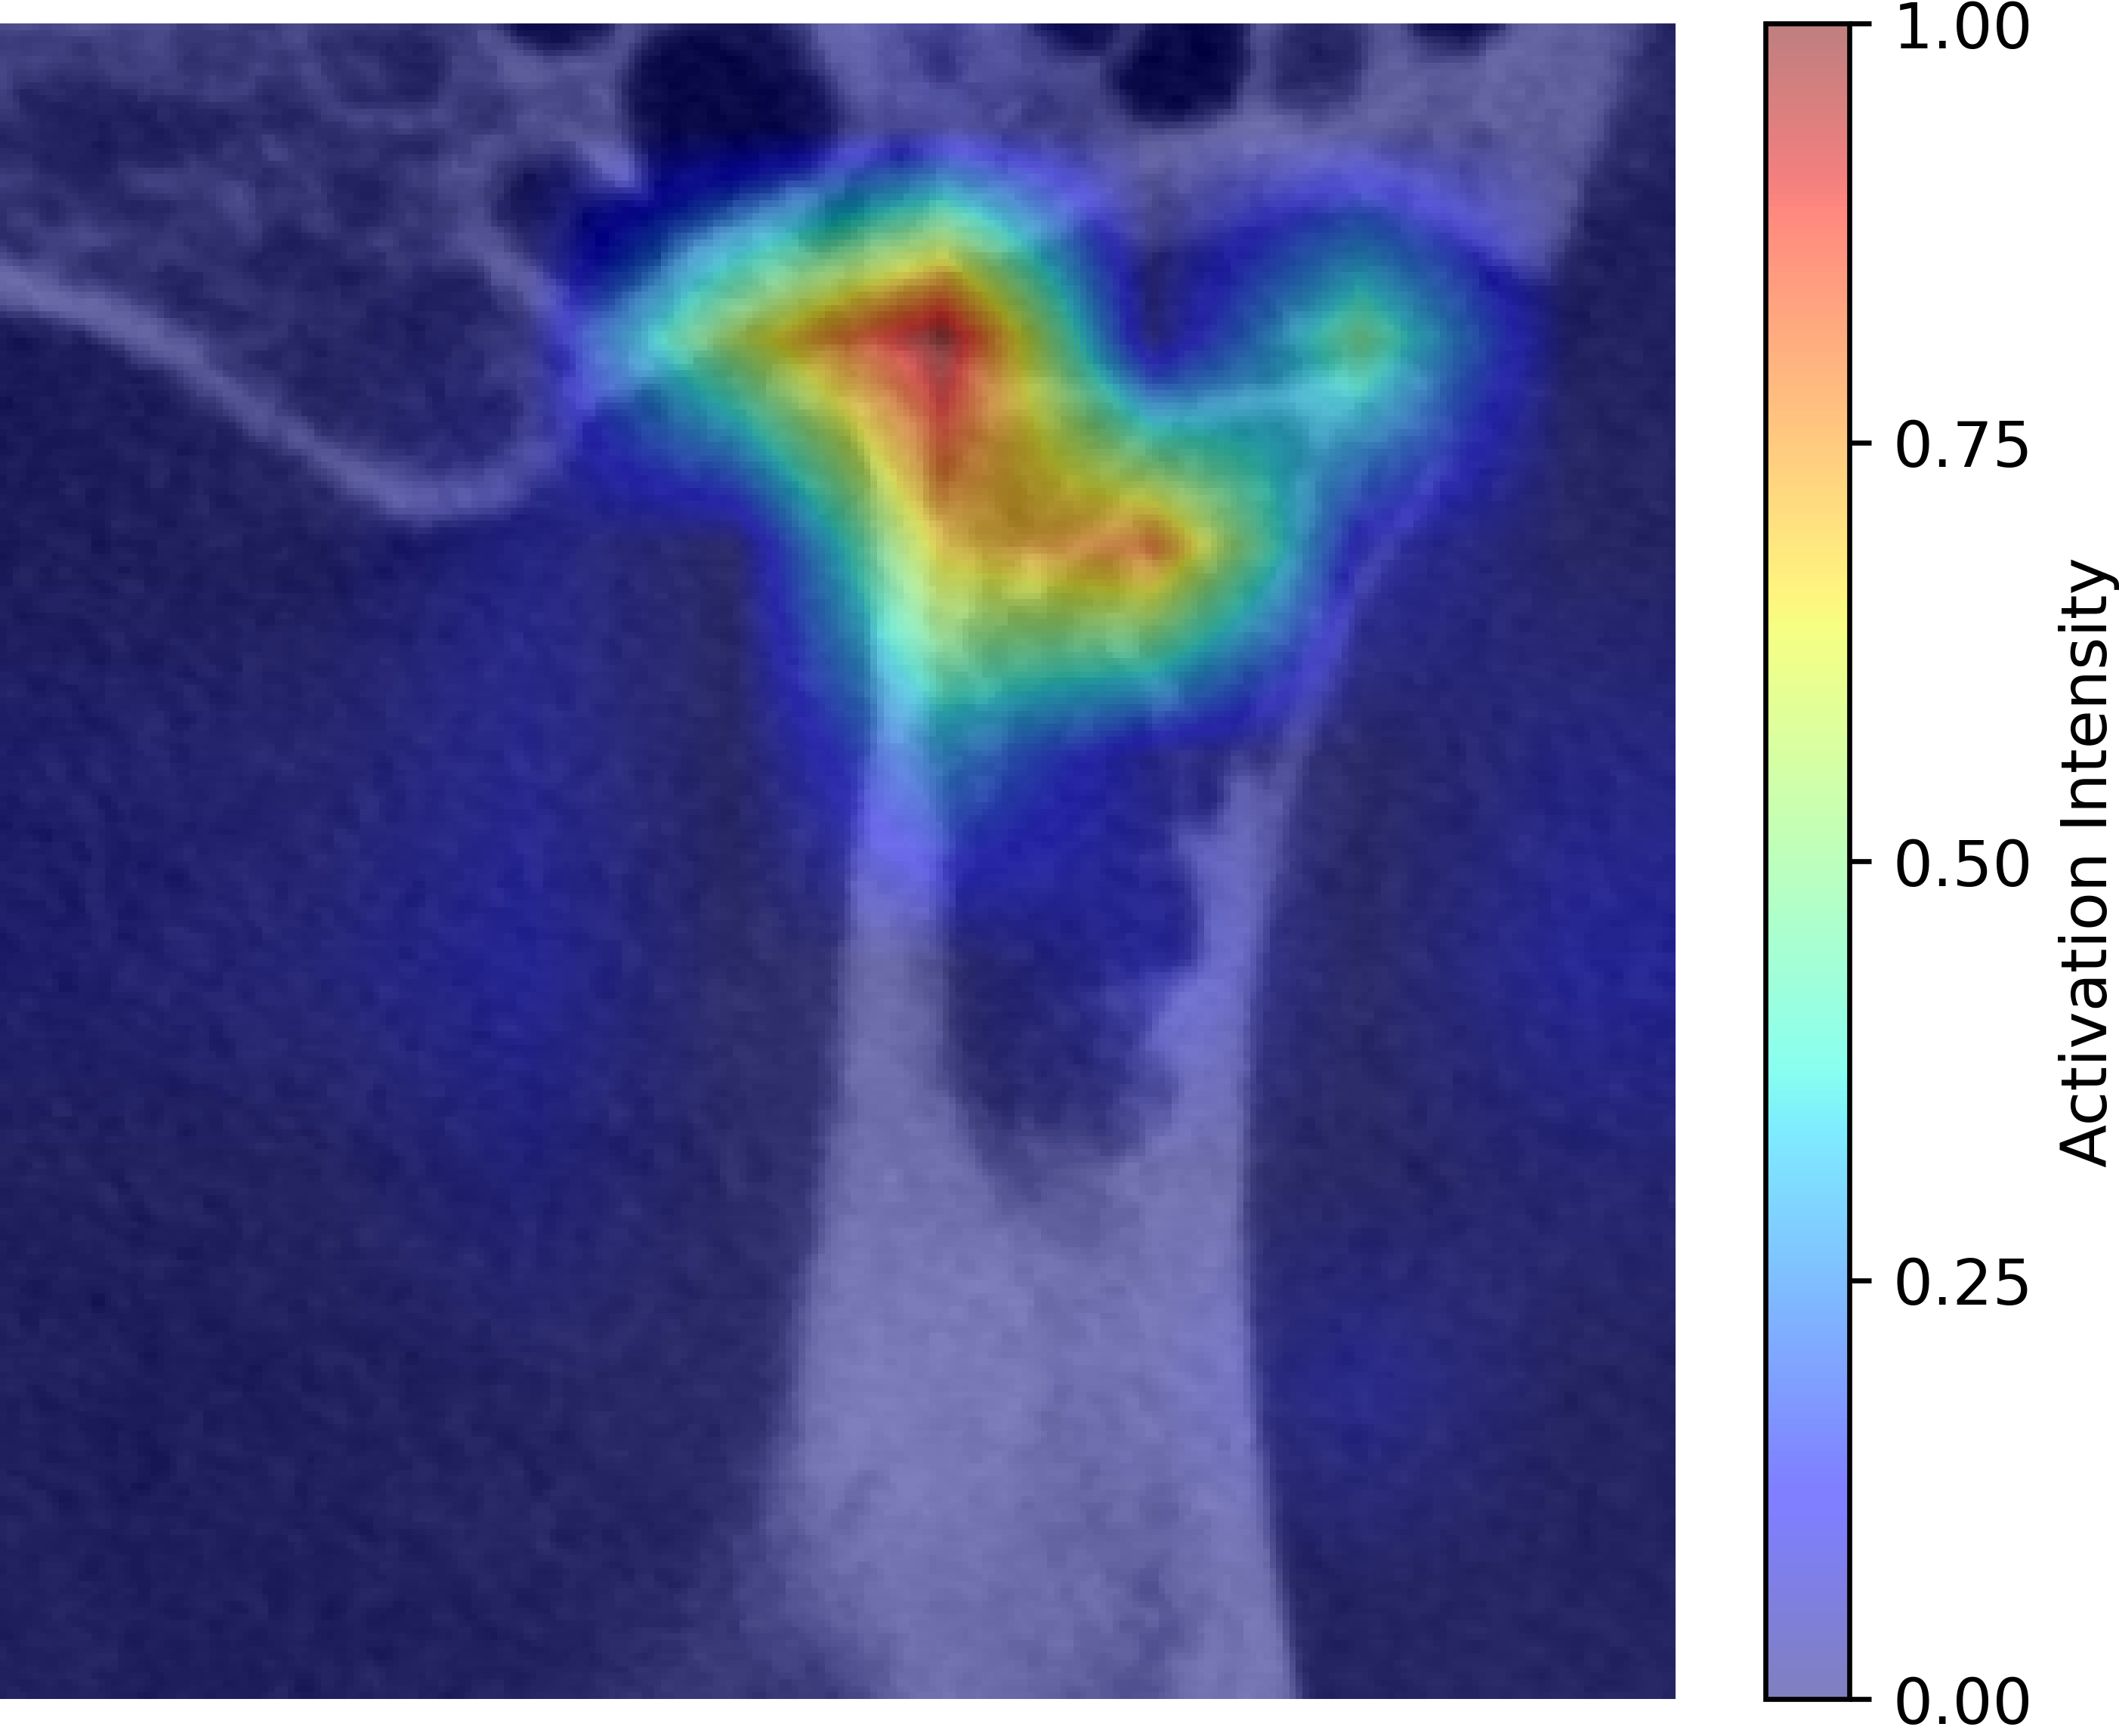
\includegraphics[width=\cellw]{figures/subCyst_overlayed_130.png} \\
  \end{tabular}
  \caption{GradCAM visualisation for ConvNeXt. (A)~Sagittal slice
  (original), and GradCAM overlays for true-positive predictions of
  (B)~Osteoarthritis, (C)~Condylar erosion, (D)~Generalised sclerosis,
  (E)~Osteophyte, and (F)~Subchondral cyst.}
  \label{fig:gradcam}
\end{figure}

\subsection{Native 3-D Baseline Comparison}
\label{sec:3d_baseline}

Table~\ref{tab:resnet_comparison} compares ResNet under the 2-D slice
sampling and native 3-D MONAI paradigms. The 3-D model achieved a
higher mean AUC-ROC (0.938 vs.\ 0.894), with the largest gains on generalised sclerosis (0.968 vs.\
0.821).

\begin{table}[htbp]
\centering
\caption{Direct comparison of ResNet across dimensionality paradigms
on the held-out test set. AUC = AUC-ROC. Per-volume GFLOPs for the 2-D
model are estimated as per-slice GFLOPs $\times$ mean retained slices
($48.36$). Best value per column in \textbf{bold}.}
\label{tab:resnet_comparison}
\small
\setlength{\tabcolsep}{4pt}
\newcolumntype{C}[1]{>{\centering\arraybackslash}p{#1}}
\begin{tabular}{l C{1.5cm} C{1.5cm} C{1.5cm} C{1.5cm} C{1.5cm} C{1.5cm} C{1.5cm}}
\toprule
\textbf{Paradigm} &
\textbf{OA} & \textbf{Erosion} & \textbf{Sclerosis} &
\textbf{Osteo.} & \textbf{Cyst} & \textbf{Mean} &
\textbf{Compute} \\
& AUC & AUC & AUC & AUC & AUC & AUC & GLOPS \\
\midrule
2-D slice sampling   & \textbf{0.980} & 0.932 & 0.821 & 0.932 & 0.805 & 0.894 & $\sim$261 \\
MONAI native 3-D     & 0.958 & \textbf{0.945} & \textbf{0.968} & \textbf{0.971} & \textbf{0.846} & \textbf{0.938} & 5{,}234 \\
\bottomrule
\end{tabular}
\end{table}

The performance advantage of the 3-D model came at a substantial
computational cost. In terms of FLOPs, the native 3-D model required
$5{,}234$~GFLOPs per volume compared with ${\sim}261$~GFLOPs for the
2-D approach, a $20$-fold difference. 

Per-volume FLOPs for the 2-D
model were estimated as the per-slice cost ($5.40$~GFLOPs) multiplied
by the mean number of retained slices after filtering and subsampling
($48.36$ across the test set). During training, the
computational gap is even wider as the 2-D approach processes only a
single sampled slice per volume at each iteration, whereas the 3-D
model must process the entire volume.

%% ===================================================================
\section{Discussion}
\label{sec:discussion}
%% ===================================================================

This study demonstrates that fully automated, multi-label classification
of TMJOA radiographic signs from CBCT is achievable with clinically
useful accuracy using standard deep learning backbones and image-level
annotations. The principal findings are discussed below.

\subsection{End-to-End Automation and Reduced Annotation Burden}

A key contribution of the proposed pipeline is the elimination of the
localisation labelling step between raw CBCT acquisition and
classification output. Prior work has commonly required bounding-box
annotation for object detection networks
\cite{talaat2023artificial,lee2020automated,Mao2025,ecser2023classification,choi2025artificial}.
By combining DentalSegmentator \cite{dot2024dentalsegmentator} for
automated mandibular segmentation with a skeletonisation-based condyle
localiser, our approach requires only image-level binary labels---the
standard output of a clinical radiological report---substantially
reducing the cost of dataset curation.

This design exploits the fact that osseous structure segmentation is a considerably
easier task for deep learning than pathology classification. Osseous
structures exhibit high contrast and well-defined boundaries that
generalise across patients, whereas classifying degenerative changes
requires distinguishing subtle morphological alterations on which even
experienced radiologists disagree (Table~\ref{tab:irr}). Empirical evidence from E\c{s}er et al.~\cite{ecser2023classification}
illustrates this gap: a single YOLOv5 model trained jointly for TMJ
segmentation and four-class OA classification on CBCT sagittal slices
achieved an AUC-ROC of 0.972 for segmentation but only
0.497 for classification, essentially chance-level performance. Similarly, Fu et al.~\cite{fu2026cbct} reported a two-stage pipeline
for CBCT-based TMJ disc displacement screening in which the
localisation stage (YOLOv11) achieved near-perfect detection
(precision 0.986, recall 0.982, mAP50 0.988), whereas the downstream
classification stage attained an AUC of only 0.733 and an accuracy of
0.669, further underscoring the disparity between localisation and
pathology classification difficulty in TMJ imaging.

By treating localisation and classification as separate stages, our
pipeline exploits the reliability of the easier task (segmentation via
DentalSegmentator) to provide a stable anatomical reference, and then allows the model to concentrate solely on the harder task (pathology classification) within a well-defined region of interest. This
separation also permits each stage to be independently improved or
replaced as more capable models become available.

\subsection{Informativeness-Weighted Slice Sampling as a Radiologist-Mimicking Strategy}

The strong performance of the informativeness-weighted
2-D slice sampling approach supports the hypothesis that this is an effective strategy for extracting
disease-relevant features from 3-D CBCT volumes using 2-D networks. The slices weighting scheme (Equation~\ref{eq:info}) mimics the radiologist's
natural tendency to select slices that pass through the bulk of the
condyle, thereby maximising the likelihood that diagnostically relevant
signs are captured within the sampled slice. The aggregated
inference (Equation~\ref{eq:agg}) then combines evidence across the
entire volume without requiring a single "best" slice to be
pre-selected, a task that is itself non-trivial to automate.

This approach parallels multiple-instance learning frameworks applied
to other volumetric imaging tasks \cite{ilse2018attention,campanella2019clinical}, but
differs in that our aggregation weights are computed from a simple
geometric prior (condylar cross-sectional area) rather than learned
attention, rendering them interpretable and computationally inexpensive.

\subsection{Architecture Insights}

ConvNeXt's frequent top ranking in bootstrap resampling is consistent
with recent benchmarks showing that modernised pure-CNN architectures
match or exceed vision transformers on medical imaging tasks with
limited training data \cite{liu2022convnet}. Nevertheless, the
substantial rank overlap among the top 10 architectures
(Figure~\ref{fig:bootstrap_rank}) indicates that this advantage is not
statistically robust at the present sample size. Large transformers
(ViT, Swin Transformer) performed competitively but did not demonstrate
clear superiority, likely reflecting their well-documented data-hungry
nature \cite{dosovitskiy2020image,raghu2021vision}. The competitive
performance of compact architectures such as MobileNet~V2 (AUC-ROC
0.914) and MobileNet~V3 (0.910) has practical implications for
deployment on commodity hardware in community dental clinics or
low-resource settings.

\subsection{2-D Slice Sampling versus Native 3-D Processing}

As reported in Section~\ref{sec:3d_baseline}, the native 3-D ResNet50
outperformed its 2-D counterpart on mean AUC-ROC (0.938 vs.\ 0.894),
with the largest gains on generalised sclerosis. This
might suggest that the morphological expression of this sign is
better captured with 3-D spatial context, though the improvement could
also reflect the substantially higher computational budget of the
volumetric model. Disentangling the contributions of spatial context
and model capacity warrants further investigation. Notably, the 3-D
model achieved this advantage despite being trained from random
initialisation, without the large-scale ImageNet pre-training that
underpins the 2-D approach. This suggests that the results reported
here may underestimate the full potential of volumetric models;
domain-specific 3-D pre-training could further widen the
performance gap.

However, the 3-D advantage must be weighed against a $20$-fold
increase in computational cost (per-volume FLOPs $5{,}234$ vs.\ ${\sim}261$~GFLOPs) and
substantially higher GPU memory requirements. Moreover, the 2-D
paradigm permits access to stronger backbone architectures. The
highest-ranked 2-D model, ConvNeXt, achieved a mean AUC-ROC of 0.926 at an
estimated ${\sim}2{,}172$~GFLOPs per volume, less than half the 3-D
cost. At the sign level, ConvNeXt surpassed the 3-D ResNet50 on OA
(0.991 vs.\ 0.958) and erosion (0.952 vs.\ 0.945), and performed
comparably on generalised sclerosis (0.944 vs.\ 0.968) and
subchondral cyst (0.823 vs.\ 0.846). The 3-D model retained a clearer
advantage only on osteophyte (0.921 vs. 0.971). Taken together, these
results indicate that a more expressive 2-D backbone can narrow or
close the gap with native volumetric processing on most signs, at a
fraction of the computational cost. This comparison illustrates a practical
advantage of the 2-D paradigm: it enables a much broader architecture
search than is currently feasible in 3-D. 

A further practical consideration is that extending modern architectures (e.g.\ ConvNeXt, Swin Transformer) to native 3-D is non-trivial: it substantially increases parameter count and memory consumption, and may render existing 2-D pretrained weights incompatible. Systematic conversion methods such as ACS convolutions \cite{yang2021reinventing} have been validated only for classical CNN families and their applicability to modern architectures remains unexplored. The 2-D slice sampling paradigm therefore remains a practical route to leveraging the full diversity of state-of-the-art ImageNet-pretrained backbones for 3-D medical imaging tasks, as demonstrated by the 20-architecture comparison in this study.

\subsection{Generalised Sclerosis and Subchondral Cyst: The Difficult Signs}

Generalised sclerosis and subchondral cyst were consistently the most difficult signs, with mean F1 scores of 0.540 and 0.616, respectively. These signs also exhibited the lowest inter-rater agreement (Fleiss' $\kappa$ = 0.664 and 0.648), suggesting that model difficulty mirrors inherent diagnostic ambiguity and that label noise places an intrinsic ceiling on attainable performance. Both signs additionally suffer from severe class imbalance and strong co-occurrence with other signs: only 1 joint in the dataset was exclusively positive for generalised sclerosis and only 2 for subchondral cyst (Figure~\ref{fig:venn}), potentially limiting the models' ability to learn sign-specific discriminative features.

\subsection{Comparison with Prior Work}

Direct numerical comparison with prior studies is complicated by differences in dataset composition, scanner characteristics, and evaluation protocols. Among detection-based approaches, Lee et al.~\cite{lee2020automated} reported accuracy of 0.86 and F1 of 0.84 using SSD on 3{,}514 manually selected slices; Talaat et al.~\cite{talaat2023artificial} achieved accuracy exceeding 95\% with YOLOv5 on 2{,}737 images; and Mao et al.~\cite{Mao2025} detected four signs with AUC values of 0.872--0.911 using YOLOv10 on 7{,}357 slices. All three required manually selected slices and per-sign bounding-box annotations, a substantially heavier annotation burden than the joint-level classification labels used in our pipeline. Among classification-based approaches, E\c{s}er et al.~\cite{ecser2023classification} achieved 0.768 classification accuracy and an F1 of 0.869 with YOLOv5 on 2{,}000 sagittal sections.

Our highest-ranked model (ConvNeXt, mean AUC-ROC 0.926; OA AUC-ROC 0.991) substantially exceeds the classification performance reported by E\c{s}er et al.\ and is comparable to the sign-level AUC values of Mao et al., while requiring neither manual slice selection nor bounding-box annotation. This demonstrates that publicly available pretrained segmentation models can effectively substitute for the labour-intensive spatial annotations demanded by detection-based approaches, without sacrificing discriminative performance.

\subsection{Limitations and Future Directions}
This is a single-centre study using one CBCT scanner, and the test set is relatively small (n=43). The informativeness weighting relies on automated segmentation quality, and clinical validation in a prospective workflow has not been performed. Because the entire pipeline depends on DentalSegmentator for both condyle localisation and informativeness scoring, segmentation errors propagate directly into downstream classification; however, the extent of this dependency has not been formally quantified. Future work should prioritise external validation on multi-centre, multi-scanner data; formal ablation of the two-stage training strategy and informativeness weighting; systematic analysis of how segmentation accuracy affects classification performance, for example by evaluating the pipeline under deliberately degraded or alternative segmentation models; exploration of 3-D architectures with domain-specific pretraining; and prospective clinical evaluation with radiologist feedback.

%% ===================================================================
\section{Conclusions}
\label{sec:conc}
%% ===================================================================

We have presented a fully automated end-to-end pipeline for multi-label
binary classification of five DC/TMD radiographic signs of
temporomandibular joint osteoarthritis from CBCT volumes. The pipeline
integrates automated mandibular segmentation, skeletonisation-based
condyle localisation, and deep learning classification without any manual
slice selection or bounding-box annotation. Among 20 architectures
evaluated, ConvNeXt achieved the highest observed mean AUC-ROC of
0.926, with near-perfect discrimination for the overall OA label
(AUC-ROC~0.991), although bootstrap resampling indicated substantial
rank overlap among the top-performing architectures. GradCAM
explainability maps confirmed that the highest-ranked models attended to
anatomically plausible condylar regions. These findings support the
feasibility of deploying this system as a computer-aided diagnosis
adjunct to conventional CBCT reporting, with the potential to reduce
diagnostic variability and accelerate large-scale TMJOA screening.

%% ===================================================================
\section*{Conflict of Interest}
The authors declare no conflict of interest.

\section*{Funding}
This research did not receive any specific grant from funding agencies
in the public, commercial, or not-for-profit sectors.

\section*{Data Availability}
The dataset used in this study is not publicly available owing to
patient confidentiality requirements. De-identified summary statistics
and model weights may be made available upon reasonable request.

\section*{Acknowledgements}
The authors thank the clinical staff at the Department of Oral and
Maxillofacial Radiology, Mahidol University Faculty of Dentistry, for
facilitating data collection.

%% ===================================================================
%% TABLES
%% ===================================================================

% \clearpage
% \begin{table}[htbp]
% \centering
% \caption{Pool of 21 candidate augmentation transformations and their
% admissible parameter ranges. For each training sample, two
% transformations are drawn uniformly at random; transformation magnitude
% is then randomised within the range shown. All transforms are sourced
% from the MONAI library \cite{monai2026}.}
% \label{tab:aug_list}
% \small
% \begin{tabular}{lll}
% \toprule
% \textbf{Category} & \textbf{Augmentation} & \textbf{Admissible Range} \\
% \midrule
% \multirow{14}{*}{Intensity}
%   & Gaussian noise          & $\text{std} \in [0, 0.03]$ \\
%   & Gaussian smooth          & $\sigma_{x,y} \in [0, 1.5]$ \\
%   & Gaussian sharpen         & $\sigma_1 \in [0, 1.0]$; $\sigma_2 \in [0, 2.0]$; $\alpha \in [0, 30]$ \\
%   & Adjust contrast          & $\gamma \in [0.7, 1.6]$ \\
%   & Shift intensity          & offset $\in [-0.1, 0.1]$ \\
%   & Scale intensity          & factor $\in [-0.2, 0.2]$ \\
%   & Bias field               & degree $\in \{1, 2, 3\}$; coeff $\in [-0.3, 0.3]$ \\
%   & Gibbs noise              & $\alpha \in [0, 0.8]$ \\
%   & K-space spike noise      & (included in pool) \\
%   & Coarse dropout           & holes $\in [1, 10]$; size $\in [1, 20]$--$[1, 40]$~px \\
%   & Coarse shuffle           & (included in pool) \\
%   & Histogram shift          & control points $\in [1, 15]$ \\
%   & Std shift intensity      & (included in pool) \\
%   & Identity                 & no transformation \\
% \midrule
% \multirow{6}{*}{Spatial}
%   & Rotation                 & $\theta \in [-30^{\circ}, +30^{\circ}]$ \\
%   & Zoom                     & scale $\in [0.8, 1.2]$ \\
%   & Affine                   & rotate $\pm 15^{\circ}$; shear $\in [-0.1, 0.1]$; translate $\pm 20$~px; scale $\in [-0.15, 0.15]$ \\
%   & 2-D elastic deformation  & rotate $\pm 10^{\circ}$; shear $\in [-0.05, 0.05]$; translate $\pm 10$~px; mag $\in [0, 2]$ \\
%   & Grid distortion          & distort limit $\in [-0.3, 0.3]$; 5 cells \\
%   & Horizontal flip          & $p = 1.0$ (when selected) \\
% \bottomrule
% \end{tabular}
% \end{table}
%% --- Table 1: Label distribution ---
% \begin{table}[htbp]
%   \centering
%   \caption{Class distribution across the training, validation, and test
%   sets for each of the five classification tasks. Note the pronounced
%   imbalance for generalised sclerosis
%   and subchondral cyst.}
%   \label{tab:label_dist}
%   \begin{tabular}{lccccccccc}
%     \hline
%     & \multicolumn{3}{c}{Training ($n=271$)} & \multicolumn{3}{c}{Validation ($n=80$)} & \multicolumn{3}{c}{Test ($n=43$)} \\
%     \cmidrule(lr){2-4} \cmidrule(lr){5-7} \cmidrule(lr){8-10}
%     Task & Pos & Neg & \% Pos & Pos & Neg & \% Pos & Pos & Neg & \% Pos \\
%     \hline
%     Osteoarthritis       & 168 & 103 & 61.99 & 45 & 35 & 56.25 & 25 & 17 & 58.14 \\
%     Erosion     & 158 & 113 & 58.30 & 36 & 44 & 45.00 & 24 & 18 & 55.81 \\
%     Generalised sclerosis & 57 & 217 & 19.93 & 8 & 72 & 10.00 & 7 & 35 & 16.28 \\
%     Osteophyte           & 132 & 139 & 48.71 & 31 & 49 & 38.75 & 19 & 23 & 44.19 \\
%     Subchondral cyst     & 91 & 180 & 33.58 & 13 & 67 & 16.25 & 13 & 29 & 30.23 \\
%     \hline
%   \end{tabular}
% \end{table}

%% --- Table 2: Inter-rater reliability ---
% \begin{table}[htbp]
% \centering
% \caption{Inter-rater reliability statistics for four TMJOA radiographic
% signs. Cohen's $\kappa$ is reported for each pairwise rater combination and
% Fleiss' $\kappa$ reflects multi-rater
% agreement.}
% \label{tab:irr}
% \small
% \begin{tabular}{lcccc}
% \toprule
% \textbf{Sign} &
% \textbf{$\kappa$ R1–R2} &
% \textbf{$\kappa$ R1–R3} &
% \textbf{$\kappa$ R2–R3} &
% \textbf{Fleiss' $\kappa$} \\
% \midrule
% Osteoarthritis     & 0.847 & 0.869 & 0.892 & 0.869 \\
% Erosion            & 0.810 & 0.852 & 0.871 & 0.844 \\
% Generalised sclerosis & 0.557 & 0.630 & 0.864 & 0.664 \\
% Osteophyte         & 0.780 & 0.803 & 0.932 & 0.837 \\
% Subchondral cyst   & 0.670 & 0.629 & 0.645 & 0.648 \\
% \bottomrule
% \end{tabular}
% \end{table}

% %% --- Table 4: Model zoo ---
% \begin{table}[htbp]
% \centering
% \caption{Architectures and Pretrained Weights evaluated.}
% \label{tab:models}
% \small
% \begin{tabular}{ll}
% \toprule
% \textbf{Architecture} &
% \textbf{Pretrained Weights} \\
% \midrule
% ConvNeXt            & ConvNeXt\_Large\_Weights.IMAGENET1K\_V1 \\
% DenseNet            & DenseNet201\_Weights.IMAGENET1K\_V1 \\
% EfficientNet        & EfficientNet\_B7\_Weights.IMAGENET1K\_V1 \\
% EfficientNet V2     & EfficientNet\_V2\_L\_Weights.IMAGENET1K\_V1 \\
% GoogLeNet           & GoogLeNet\_Weights.IMAGENET1K\_V1 \\
% Inception V3        & Inception\_V3\_Weights.IMAGENET1K\_V1 \\
% MaxViT              & MaxVit\_T\_Weights.IMAGENET1K\_V1 \\
% MNASNet             & MNASNet1\_3\_Weights.IMAGENET1K\_V1 \\
% MobileNet V2        & MobileNet\_V2\_Weights.IMAGENET1K\_V2 \\
% MobileNet V3        & MobileNet\_V3\_Large\_Weights.IMAGENET1K\_V2 \\
% RegNetX             & RegNet\_X\_32GF\_Weights.IMAGENET1K\_V2 \\
% RegNetY             & RegNet\_Y\_128GF\_Weights.IMAGENET1K\_SWAG\_E2E\_V1 \\
% ResNet              & ResNet152\_Weights.IMAGENET1K\_V2 \\
% ResNeXt             & ResNeXt101\_64X4D\_Weights.IMAGENET1K\_V1 \\
% ShuffleNet V2       & ShuffleNet\_V2\_X2\_0\_Weights.IMAGENET1K\_V1 \\
% Swin Transformer    & Swin\_B\_Weights.IMAGENET1K\_V1 \\
% Swin Transformer V2 & Swin\_V2\_B\_Weights.IMAGENET1K\_V1 \\
% VGG                 & VGG19\_BN\_Weights.IMAGENET1K\_V1 \\
% Vision Transformer  & ViT\_L\_16\_Weights.IMAGENET1K\_SWAG\_E2E\_V1 \\
% YOLOv11             & yolo11x-cls \\
% \bottomrule
% \end{tabular}
% \end{table}

%% --- Table 5: Full results Protocol 1 ---
% \begin{sidewaystable}[htbp]
% \centering
% \caption{Test-set performance of all 20 architectures using
% informativeness-weighted 2-D slice sampling. Best value per column in
% \textbf{bold}$^{*}$. Acc = accuracy; P = precision; R = recall; AUC = AUC-ROC.}
% \label{tab:results_p1}
% \scriptsize
% \setlength{\tabcolsep}{3pt}
% \begin{tabular}{l rrrrr rrrrr rrrrr rrrrr rrrrr}
% \toprule
% & \multicolumn{5}{c}{\textbf{OA}}
% & \multicolumn{5}{c}{\textbf{Erosion}}
% & \multicolumn{5}{c}{\textbf{Generalised sclerosis}}
% & \multicolumn{5}{c}{\textbf{Osteophyte}}
% & \multicolumn{5}{c}{\textbf{Subchondral cyst}} \\
% \cmidrule(lr){2-6}\cmidrule(lr){7-11}\cmidrule(lr){12-16}\cmidrule(lr){17-21}\cmidrule(lr){22-26}
% \textbf{Model}
% & Acc & P & R & F1 & AUC
% & Acc & P & R & F1 & AUC
% & Acc & P & R & F1 & AUC
% & Acc & P & R & F1 & AUC
% & Acc & P & R & F1 & AUC \\
% \midrule
% ConvNeXt       & \textbf{.95}* & .93 & \textbf{1.0}* & \textbf{.96}* & \textbf{.99}* & \textbf{.91}* & \textbf{.95}* & .88 & .91 & \textbf{.95}* & .63 & .30 & \textbf{1.0}* & .47 & .94 & \textbf{.86}* & \textbf{.81}* & .89 & \textbf{.85}* & .92 & .72 & .53 & .77 & .62 & .82 \\
% DenseNet       & .91 & .89 & .96 & .92 & \textbf{.99}* & .81 & .75 & \textbf{1.0}* & .86 & \textbf{.95}* & .84 & .50 & .86 & .63 & .91 & .77 & .67 & .95 & .78 & .92 & .72 & .52 & .92 & \textbf{.67}* & .84 \\
% EfficientNet   & .93 & .92 & .96 & .94 & .97 & .88 & .88 & .92 & .90 & .91 & .74 & .38 & .86 & .52 & .88 & .79 & .69 & .95 & .80 & .94 & .63 & .43 & .77 & .56 & .78 \\
% EfficientNet V2 & .91 & .86 & \textbf{1.0}* & .93 & .97 & .81 & .81 & .88 & .84 & .93 & .81 & .47 & \textbf{1.0}* & .64 & .90 & .77 & .68 & .89 & .77 & .92 & .72 & .52 & .92 & \textbf{.67}* & .83 \\
% GoogLeNet      & .91 & .86 & \textbf{1.0}* & .93 & .98 & .88 & .83 & \textbf{1.0}* & .91 & .93 & .81 & .47 & \textbf{1.0}* & .64 & .93 & .72 & .63 & .89 & .74 & .91 & .65 & .46 & .92 & .62 & .82 \\
% Inception V3   & .91 & .89 & .96 & .92 & .97 & .84 & .81 & .92 & .86 & .94 & .77 & .41 & \textbf{1.0}* & .58 & .91 & .74 & .65 & .89 & .76 & .93 & .58 & .42 & \textbf{1.0}* & .59 & \textbf{.85}* \\
% MaxViT         & .88 & .92 & .88 & .90 & .97 & .88 & .88 & .92 & .90 & .92 & .77 & .41 & \textbf{1.0}* & .58 & .88 & .74 & .65 & .89 & .76 & .94 & .70 & .50 & .92 & .65 & .82 \\
% MNASNet        & .86 & .83 & .96 & .89 & .95 & .84 & .79 & .96 & .87 & .93 & .67 & .33 & \textbf{1.0}* & .50 & .89 & .77 & .68 & .89 & .77 & .89 & .60 & .42 & .77 & .54 & .80 \\
% MobileNet V2   & .93 & \textbf{.96}* & .92 & .94 & .98 & .86 & .85 & .92 & .88 & .93 & \textbf{.86}* & \textbf{.55}* & .86 & \textbf{.67}* & .93 & .74 & .65 & .89 & .76 & .90 & .70 & .50 & .85 & .63 & .83 \\
% MobileNet V3   & .91 & .86 & \textbf{1.0}* & .93 & .98 & \textbf{.91}* & .92 & .92 & \textbf{.92}* & \textbf{.95}* & .65 & .32 & \textbf{1.0}* & .48 & .89 & .79 & .69 & .95 & .80 & .92 & .65 & .46 & \textbf{1.0}* & .63 & .81 \\
% RegNetX        & .88 & .86 & .96 & .91 & .98 & \textbf{.91}* & .86 & \textbf{1.0}* & \textbf{.92}* & .94 & .84 & .50 & .71 & .59 & .92 & .81 & .74 & .89 & .81 & .93 & .65 & .46 & .85 & .59 & .81 \\
% RegNetY        & .81 & .81 & .88 & .85 & .95 & .79 & .80 & .83 & .82 & .91 & .74 & .38 & .86 & .52 & .84 & .72 & .63 & .89 & .74 & .89 & .63 & .44 & .92 & .60 & .76 \\
% ResNet         & .91 & .86 & \textbf{1.0}* & .93 & .98 & \textbf{.91}* & .88 & .96 & \textbf{.92}* & .93 & .65 & .28 & .71 & .40 & .82 & .84 & .75 & .95 & .84 & .93 & \textbf{.74}* & \textbf{.56}* & .69 & .62 & .81 \\
% ResNeXt        & .91 & .92 & .92 & .92 & .98 & .88 & .91 & .88 & .89 & .94 & .70 & .35 & \textbf{1.0}* & .52 & .90 & .79 & .71 & .89 & .79 & .92 & .67 & .48 & \textbf{1.0}* & .65 & .84 \\
% ShuffleNet V2  & .81 & .76 & \textbf{1.0}* & .86 & .96 & .86 & .85 & .92 & .88 & .91 & .74 & .39 & \textbf{1.0}* & .56 & .92 & .79 & .71 & .89 & .79 & .92 & .60 & .42 & .85 & .56 & .78 \\
% Swin Trans.    & .86 & .85 & .92 & .88 & .96 & .88 & .88 & .92 & .90 & .93 & .58 & .28 & \textbf{1.0}* & .44 & \textbf{.96}* & .79 & .71 & .89 & .79 & .92 & .70 & .50 & .92 & .65 & .83 \\
% Swin Trans.\ V2 & .91 & .89 & .96 & .92 & .97 & .88 & .85 & .96 & .90 & .92 & .74 & .39 & \textbf{1.0}* & .56 & .92 & \textbf{.86}* & \textbf{.81}* & .89 & \textbf{.85}* & .92 & .63 & .43 & .77 & .56 & .84 \\
% VGG            & .88 & .92 & .88 & .90 & .97 & .81 & .83 & .83 & .83 & .92 & .56 & .27 & \textbf{1.0}* & .42 & .94 & .74 & .65 & .89 & .76 & .92 & .67 & .48 & .85 & .61 & .83 \\
% ViT            & .88 & .83 & \textbf{1.0}* & .91 & .98 & \textbf{.91}* & .92 & .92 & \textbf{.92}* & .94 & .74 & .39 & \textbf{1.0}* & .56 & .89 & .81 & .70 & \textbf{1.0}* & .83 & \textbf{.95}* & .70 & .50 & .85 & .63 & .84 \\
% YOLOv11        & .88 & .86 & .96 & .91 & .98 & .88 & .88 & .92 & .90 & .94 & .70 & .35 & \textbf{1.0}* & .52 & .92 & .77 & .67 & .95 & .78 & .91 & .70 & .50 & \textbf{1.0}* & \textbf{.67}* & .84 \\
% \midrule
% \textbf{Mean}  & .892 & .874 & .956 & .913 & .973 & .867 & .857 & .923 & .887 & .931 & .727 & .386 & .943 & .540 & .905 & .781 & .694 & .911 & .789 & .920 & .668 & .477 & .877 & .616 & .819 \\
% \bottomrule
% \end{tabular}
% \end{sidewaystable}

% \begin{table}[htbp]
% \centering
% \caption{Test-set AUC-ROC for all 20 architectures across five tasks,
% sorted by mean AUC-ROC. Best value per column in \textbf{bold}. Full
% results including accuracy, precision, recall, and F1 are provided in
% Supplementary Table~S1.}
% \label{tab:model_summary}
% \small
% \setlength{\tabcolsep}{5pt}
% \begin{tabular}{lcccccc}
% \toprule
% \textbf{Model} & \textbf{OA} & \textbf{Erosion} & \textbf{Scle.} & \textbf{Osteo.} & \textbf{S.\ Cyst} & \textbf{Mean} \\
% \midrule
% ConvNeXt            & \textbf{0.991} & \textbf{0.952} & 0.944 & 0.921 & 0.823 & \textbf{0.926} \\
% DenseNet            & 0.987 & 0.945 & 0.913 & 0.923 & 0.836 & 0.921 \\
% ViT                 & 0.980 & 0.939 & 0.893 & \textbf{0.950} & 0.841 & 0.920 \\
% Inception V3        & 0.978 & 0.936 & 0.909 & 0.925 & \textbf{0.849} & 0.919 \\
% ResNeXt             & 0.984 & 0.943 & 0.909 & 0.921 & 0.839 & 0.919 \\
% Swin Transformer    & 0.964 & 0.925 & \textbf{0.956} & 0.917 & 0.828 & 0.918 \\
% YOLOv11             & 0.980 & 0.939 & 0.917 & 0.906 & 0.844 & 0.917 \\
% VGG                 & 0.971 & 0.923 & 0.937 & 0.917 & 0.828 & 0.915 \\
% Swin Transformer V2 & 0.969 & 0.923 & 0.925 & 0.921 & 0.836 & 0.915 \\
% RegNetX             & 0.978 & 0.939 & 0.921 & 0.925 & 0.808 & 0.914 \\
% MobileNet V2        & 0.976 & 0.925 & 0.929 & 0.904 & 0.833 & 0.913 \\
% GoogLeNet           & 0.976 & 0.930 & 0.929 & 0.906 & 0.823 & 0.913 \\
% MobileNet V3        & 0.984 & 0.945 & 0.893 & 0.919 & 0.808 & 0.910 \\
% EfficientNet V2     & 0.969 & 0.925 & 0.901 & 0.923 & 0.826 & 0.909 \\
% MaxViT              & 0.971 & 0.921 & 0.877 & 0.941 & 0.821 & 0.906 \\
% ShuffleNet V2       & 0.960 & 0.912 & 0.921 & 0.921 & 0.780 & 0.899 \\
% EfficientNet        & 0.969 & 0.910 & 0.885 & 0.936 & 0.782 & 0.896 \\
% ResNet              & 0.980 & 0.932 & 0.821 & 0.932 & 0.805 & 0.894 \\
% MNASNet             & 0.951 & 0.930 & 0.893 & 0.886 & 0.800 & 0.892 \\
% RegNetY             & 0.951 & 0.908 & 0.837 & 0.893 & 0.767 & 0.871 \\
% \midrule
% \textbf{Mean}       & 0.973 & 0.930 & 0.905 & 0.919 & 0.819 & 0.909 \\
% \bottomrule
% \end{tabular}
% \end{table}

%% --- Table 6 : Model-level summary (sorted by AUC-ROC descending) ---
% \begin{table}[htbp]
% \centering
% \caption{Summary performance of all 20 architectures, averaged across five tasks
% and sorted by mean AUC-ROC. Acc = accuracy; P = precision;
% R = recall; AUC = AUC-ROC. Best value per column in \textbf{bold}.}
% \label{tab:model_summary}
% \small
% \begin{tabular}{lccccc}
% \toprule
% \textbf{Model} & \textbf{Acc} & \textbf{P} & \textbf{R} & \textbf{F1} & \textbf{AUC} \\
% \midrule
% ConvNeXt            & 0.814 & \textbf{0.704} & 0.908 & 0.762 & \textbf{0.926} \\
% DenseNet            & 0.810 & 0.666 & 0.938 & \textbf{0.772} & 0.922 \\
% Swin Transformer    & 0.762 & 0.644 & 0.930 & 0.732 & 0.920 \\
% Vision Transformer  & 0.808 & 0.668 & 0.954 & 0.770 & 0.920 \\
% Inception V3        & 0.702 & 0.574 & 0.962 & 0.706 & 0.920 \\
% YOLOv11             & 0.786 & 0.652 & 0.966 & 0.756 & 0.918 \\
% RegNetX             & \textbf{0.818} & 0.684 & 0.882 & 0.764 & 0.916 \\
% ResNeXt             & 0.790 & 0.674 & 0.938 & 0.754 & 0.916 \\
% VGG                 & 0.732 & 0.630 & 0.890 & 0.704 & 0.916 \\
% GoogLeNet           & 0.794 & 0.650 & 0.962 & 0.768 & 0.914 \\
% MobileNet V2        & \textbf{0.818} & 0.702 & 0.888 & 0.776 & 0.914 \\
% Swin Transformer V2 & 0.804 & 0.674 & 0.916 & 0.758 & 0.914 \\
% EfficientNet V2     & 0.804 & 0.668 & 0.938 & 0.770 & 0.910 \\
% MobileNet V3        & 0.782 & 0.650 & \textbf{0.974} & 0.752 & 0.910 \\
% MaxViT              & 0.794 & 0.672 & 0.922 & 0.758 & 0.906 \\
% ShuffleNet V2       & 0.760 & 0.626 & 0.932 & 0.730 & 0.898 \\
% EfficientNet        & 0.794 & 0.660 & 0.892 & 0.744 & 0.896 \\
% ResNet              & 0.810 & 0.666 & 0.862 & 0.742 & 0.894 \\
% MNASNet             & 0.748 & 0.610 & 0.916 & 0.714 & 0.892 \\
% RegNetY             & 0.738 & 0.612 & 0.876 & 0.706 & 0.870 \\
% \bottomrule
% \end{tabular}
% \end{table}

%% --- Table 7: Task-level summary ---
% \begin{table}[htbp]
% \centering
% \caption{Mean test-set performance across all 20 architectures for each
% classification task. Acc = accuracy; P = precision; R = recall;
% AUC = AUC-ROC. Best value per column in \textbf{bold}.}
% \label{tab:task_summary}
% \small
% \begin{tabular}{lccccc}
% \toprule
% \textbf{Task} & \textbf{Acc} & \textbf{P} & \textbf{R} & \textbf{F1} & \textbf{AUC} \\
% \midrule
% Osteoarthritis        & \textbf{0.892} & \textbf{0.874} & 0.956 & \textbf{0.913} & \textbf{0.973} \\
% Erosion      & 0.867 & 0.857 & 0.923 & 0.887 & 0.931 \\
% Osteophyte            & 0.781 & 0.694 & 0.911 & 0.789 & 0.920 \\
% Generalised sclerosis & 0.727 & 0.386 & \textbf{0.943} & 0.540 & 0.905 \\
% Subchondral cyst      & 0.668 & 0.477 & 0.877 & 0.616 & 0.819 \\
% \bottomrule
% \end{tabular}
% \end{table}

%% --- Table 8: 2D vs 3D comparison ---
% \begin{table}[htbp]
% \centering
% \caption{Direct comparison of ResNet50 across dimensionality
% paradigms on the held-out test set. AUC = AUC-ROC. Best value per
% column in \textbf{bold}.}
% \label{tab:resnet_comparison}
% \small
% \setlength{\tabcolsep}{4pt}
% \newcolumntype{C}[1]{>{\centering\arraybackslash}p{#1}}
% \begin{tabular}{l C{1.5cm} C{1.5cm} C{1.5cm} C{1.5cm} C{1.5cm} C{1.5cm}}
% \toprule
% \textbf{Paradigm} &
% \textbf{OA} & \textbf{Erosion} & \textbf{Scle.} &
% \textbf{Osteo.} & \textbf{S.\ Cyst} & \textbf{Mean} \\
% & AUC & AUC & AUC & AUC & AUC & AUC \\
% \midrule
% 2-D slice sampling   & \textbf{0.962} & 0.941 & 0.941 & 0.928 & 0.831 & 0.920 \\
% MONAI native 3-D     & 0.958 & \textbf{0.945} & \textbf{0.968} & \textbf{0.971} & \textbf{0.846} & \textbf{0.938} \\
% \bottomrule
% \end{tabular}
% \end{table}

% \begin{table}[htbp]
% \centering
% \caption{Direct comparison of ResNet50 across dimensionality paradigms
% on the held-out test set. AUC = AUC-ROC. Per-volume GFLOPs for the 2-D
% model are estimated as per-slice GFLOPs $\times$ mean retained slices
% ($48.36$). Best value per column in \textbf{bold}.}
% \label{tab:resnet_comparison}
% \small
% \setlength{\tabcolsep}{4pt}
% \newcolumntype{C}[1]{>{\centering\arraybackslash}p{#1}}
% \begin{tabular}{l C{1.5cm} C{1.5cm} C{1.5cm} C{1.5cm} C{1.5cm} C{1.5cm} C{1.5cm}}
% \toprule
% \textbf{Paradigm} &
% \textbf{OA} & \textbf{Erosion} & \textbf{Scle.} &
% \textbf{Osteo.} & \textbf{S.\ Cyst} & \textbf{Mean} &
% \textbf{Compute} \\
% & AUC & AUC & AUC & AUC & AUC & AUC & GLOPS \\
% \midrule
% 2-D slice sampling   & \textbf{0.962} & 0.941 & 0.941 & 0.928 & 0.831 & 0.920 & $\sim$261 \\
% MONAI native 3-D     & 0.958 & \textbf{0.945} & \textbf{0.968} & \textbf{0.971} & \textbf{0.846} & \textbf{0.938} & 5{,}234 \\
% \bottomrule
% \end{tabular}
% \end{table}

%% ===================================================================
%% FIGURES
%% ===================================================================

\clearpage

% %% --- Figure 1: Venn diagram ---
% \begin{figure}[htbp]
%   \centering
%   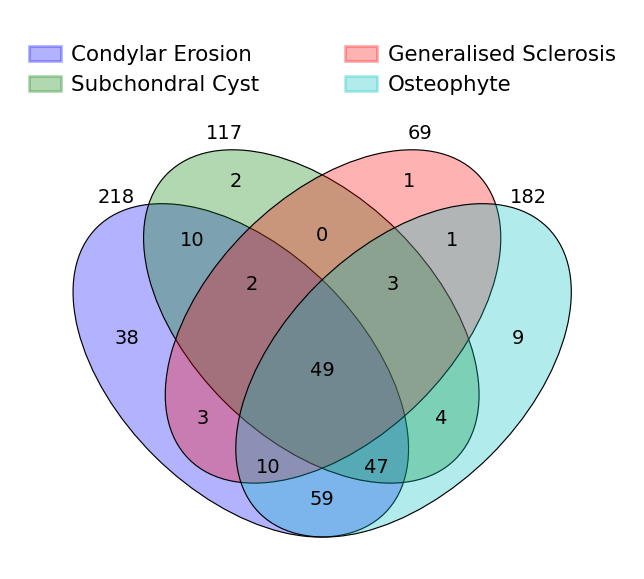
\includegraphics[width=0.5\textwidth]{figures/Venn.png}
%   \caption{Four-set Venn diagram illustrating the co-occurrence of
%   condylar erosion, generalised sclerosis, osteophyte, and subchondral
%   cyst among the OA-positive joints in the full dataset.}
%   \label{fig:venn}
% \end{figure}

%% --- Figure 2: Preprocess pipeline ---
% \begin{figure}[htbp]
%   \centering
%   \includegraphics[width=0.8\textwidth]{figures/preproces_pipeline.pdf}
%   \caption{Preprocessing pipeline for condylar volume extraction. (A)~Raw CBCT volume acquired on a 3D Accuitomo XYZ scanner. (B)~Automatic mandibular segmentation using DentalSegmentator. (C)~Condyle-centred cropping via 3-D skeletonisation of the mandibular mask.}
%   \label{fig:preprocessing_pipeline}
% \end{figure}

% \begin{figure}[htbp]
%   \centering
%   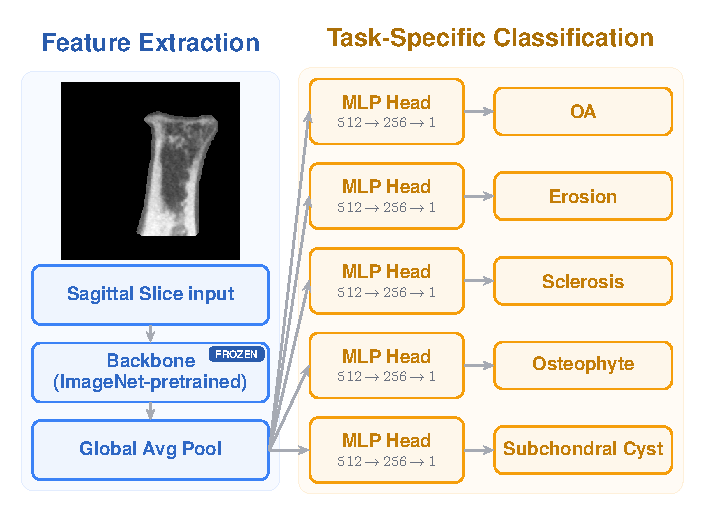
\includegraphics[width=0.8\textwidth]{figures/architecture_pipeline.pdf}
%   \caption{Classification framework architecture. Left: the feature
%   extraction pipeline consisting of a sagittal slice input, a frozen
%   ImageNet-pretrained backbone, and global average pooling. Right: five
%   task-specific MLP heads ($512 \to 256 \to 1$ with ReLU and dropout
%   $p = 0.3$), one per DC/TMD sign.}
%   \label{fig:model_architecture}
% \end{figure}

% \begin{figure}[htbp]
%   \centering
%   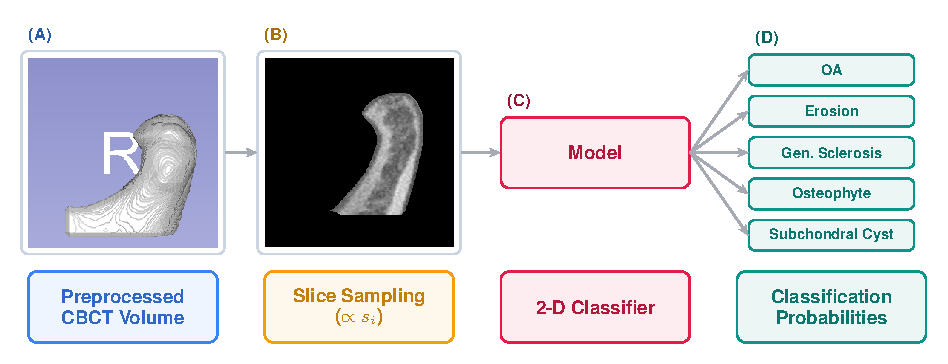
\includegraphics[width=0.9\textwidth]{figures/train_pipeline.pdf}
%   \caption{Inference process during training. (A)~Preprocessed CBCT volume input. (B)~A single sagittal slice is sampled with probability proportional to its informativeness score~$s_i$. (C)~The sampled slice is passed through the model. (D)~Five independent binary classification outputs.}
%   \label{fig:training_pipeline}
% \end{figure}

% \begin{figure}[htbp]
%   \centering
%   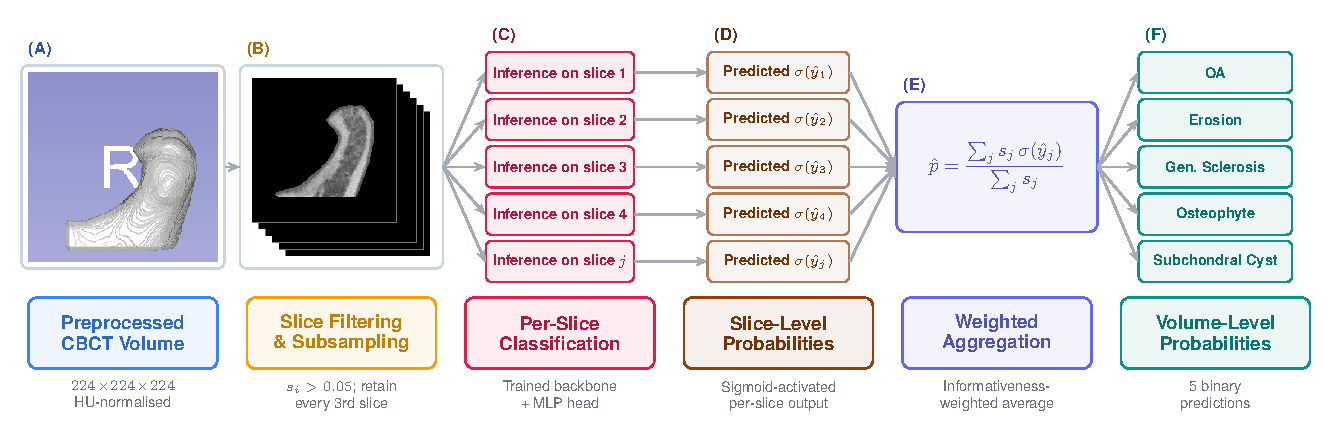
\includegraphics[width=0.9\textwidth]{figures/inference_pipeline.pdf}
%   \caption{Inference process in deployment. (A)~Preprocessed CBCT volume input. (B)~Sagittal slices are filtered and subsampled. (C)~Each retained slice is independently classified by the trained model. (D)~Slice-level sigmoid probabilities output $\sigma(\hat{y}_j)$. (E)~Informativeness-weighted aggregation produces volume-level probability $\hat{p}$ (Equation~\ref{eq:agg}). (F)~Final binary predictions.}
%   \label{fig:inference_pipeline}
% \end{figure}

% \begin{figure}[htbp]
%   \centering
%   \newlength{\cellw}
%   \setlength{\cellw}{0.32\textwidth}
%   \newcolumntype{L}{>{\raggedright\arraybackslash}p{\cellw}}
%   \begin{tabular}{@{}LLL@{}}
%     \textbf{(A)} & \textbf{(B)} & \textbf{(C)} \\[-2pt]
%     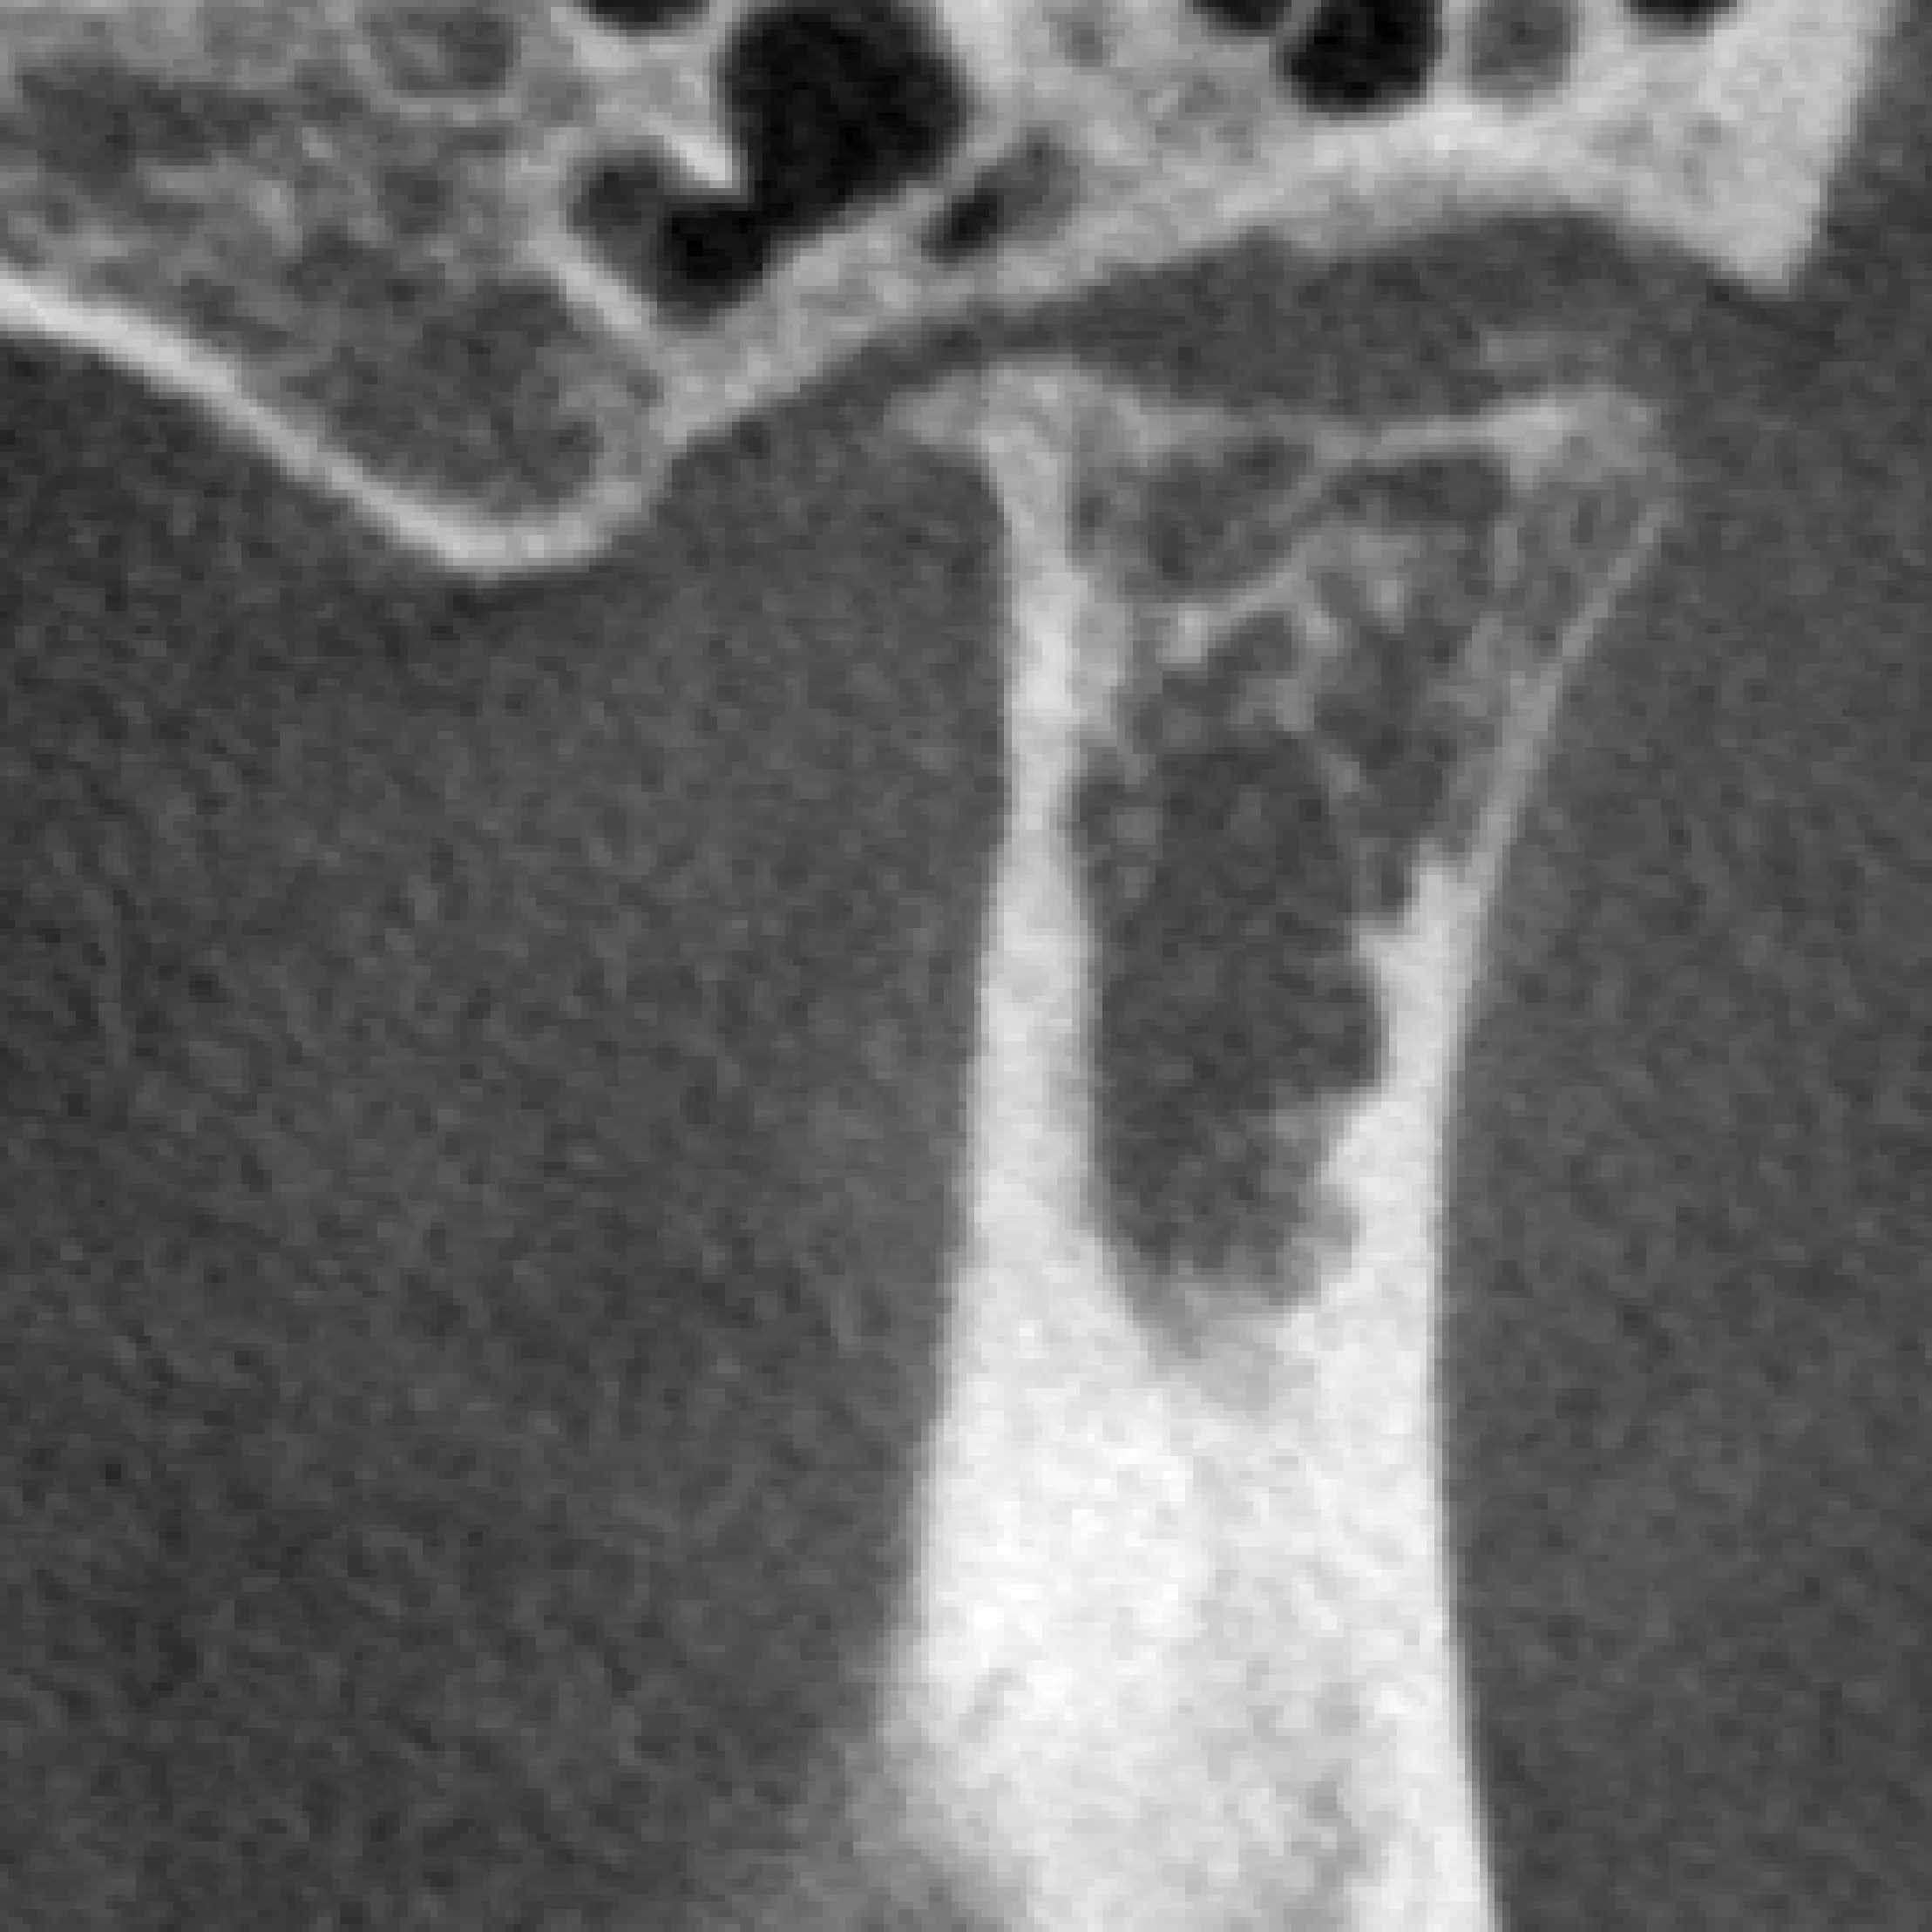
\includegraphics[width=0.81\cellw]{figures/original_130.png} &
%     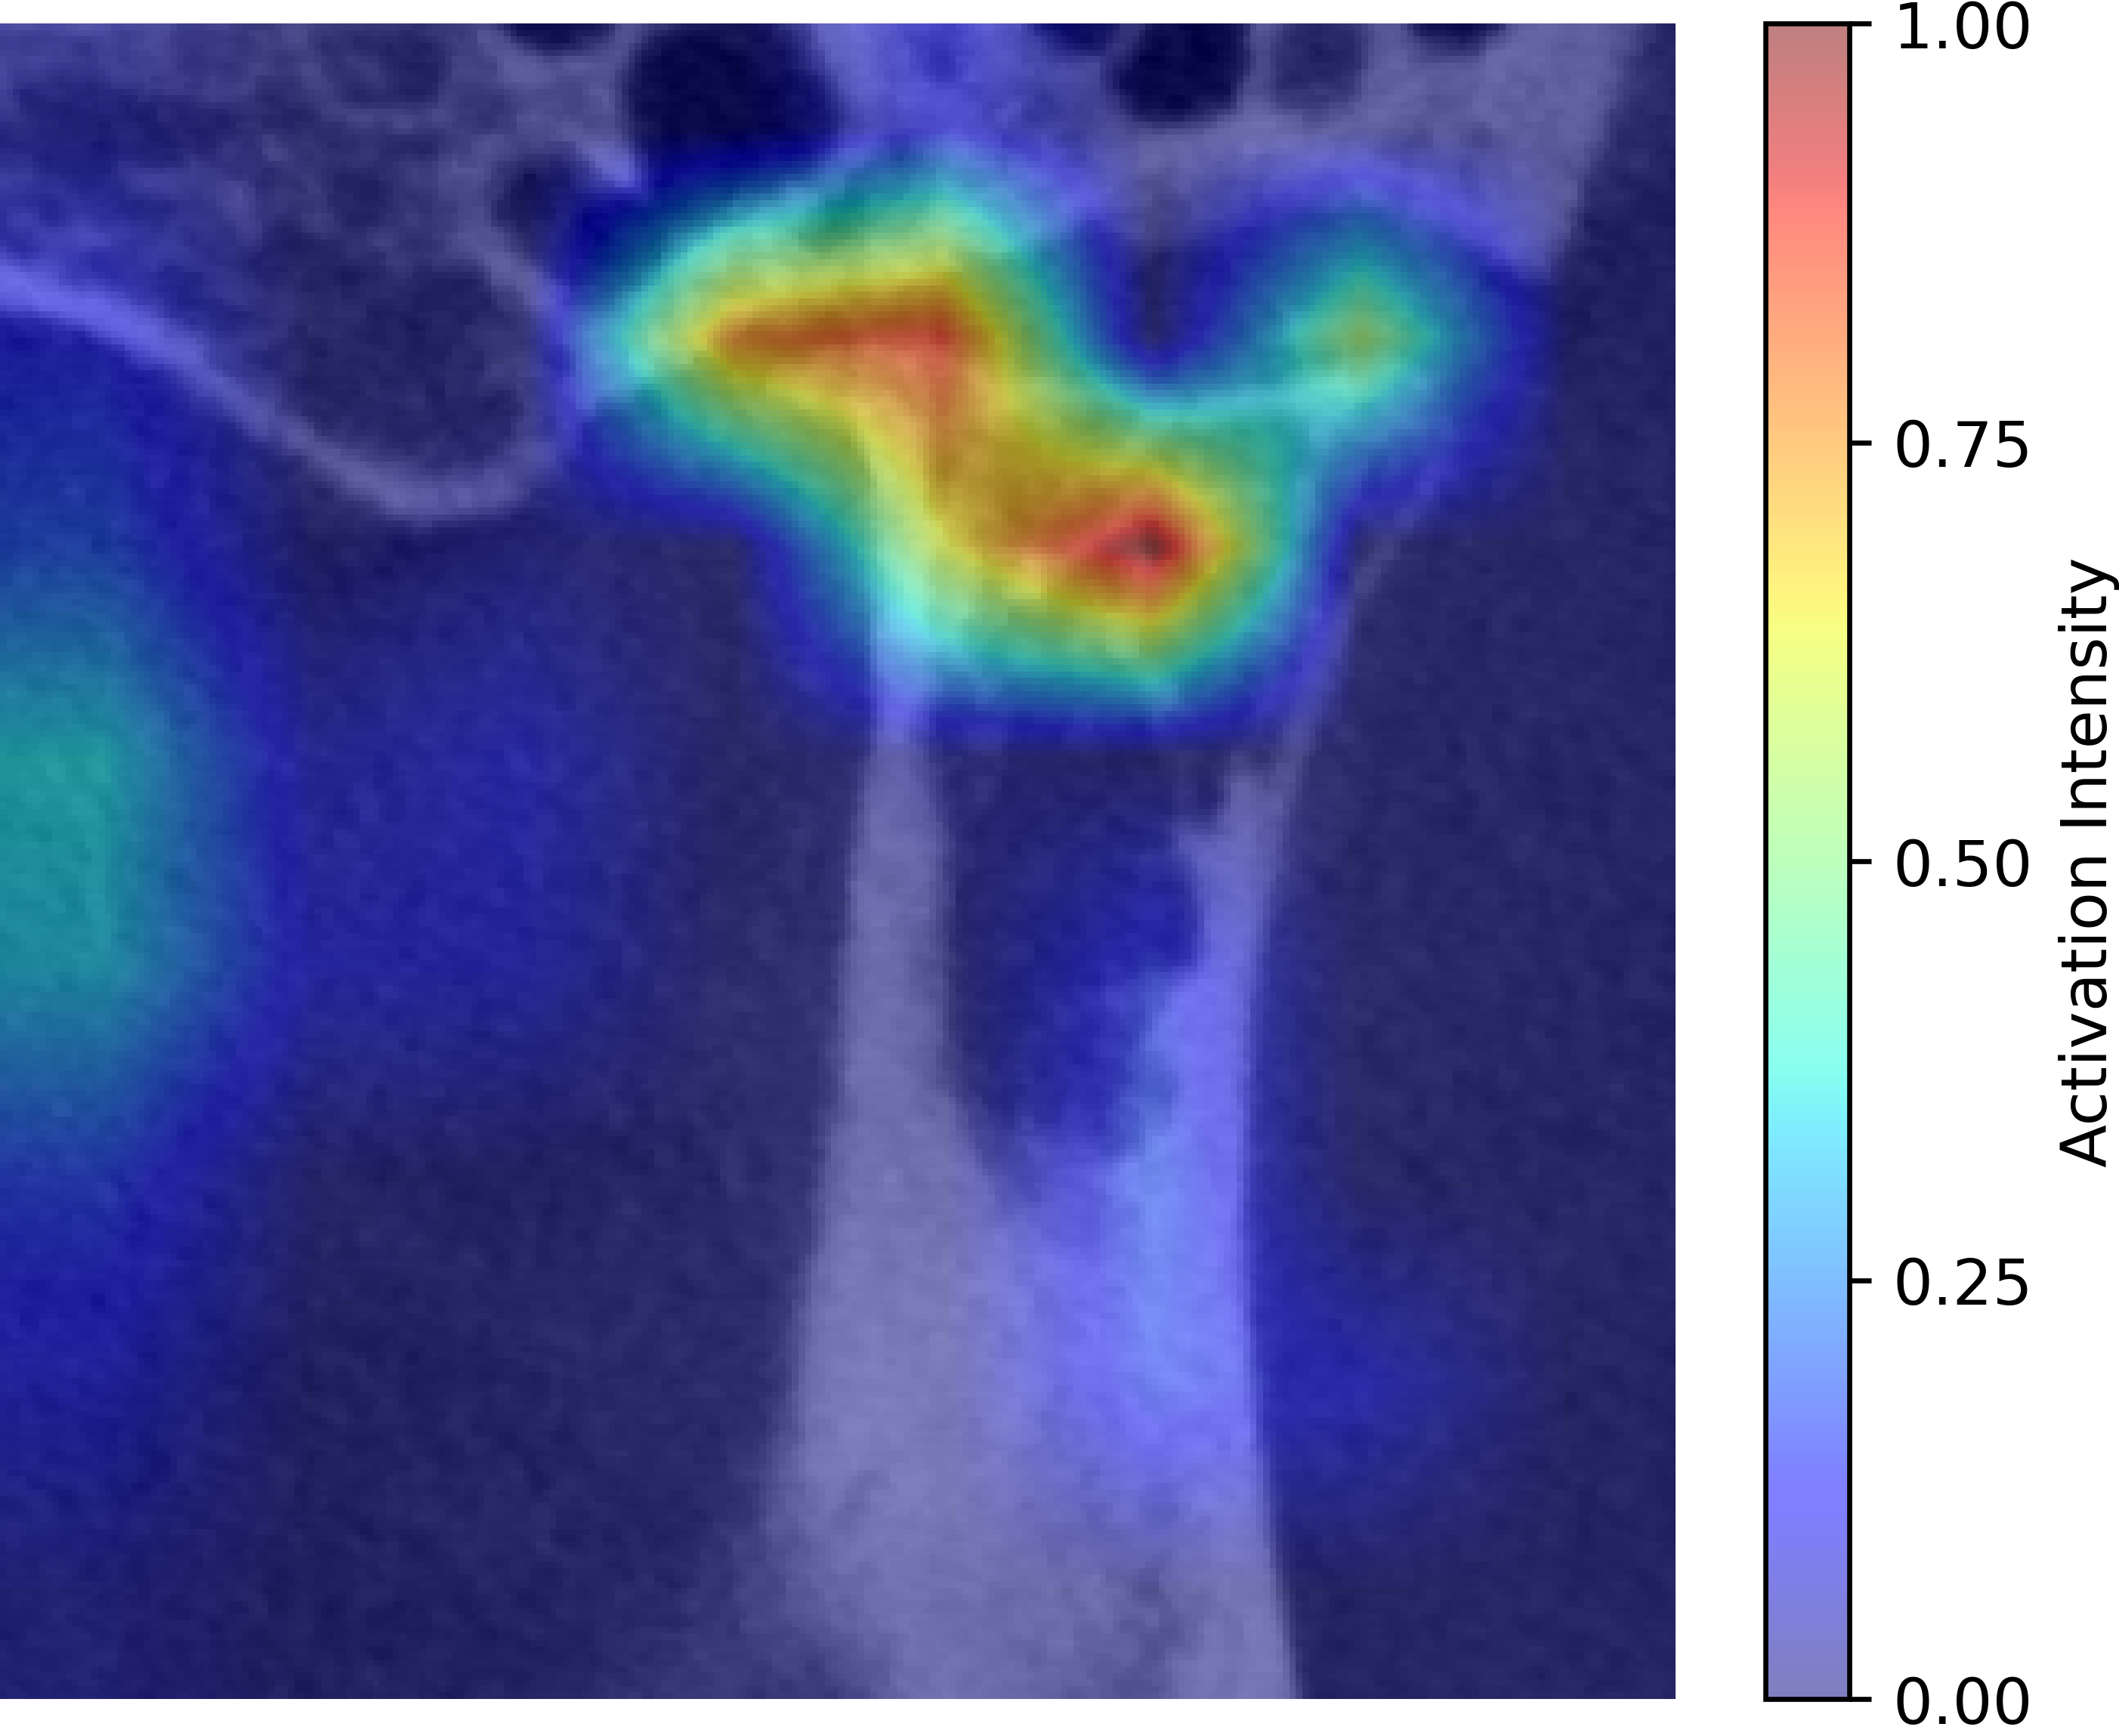
\includegraphics[width=\cellw]{figures/OA_overlayed_130.png} &
%     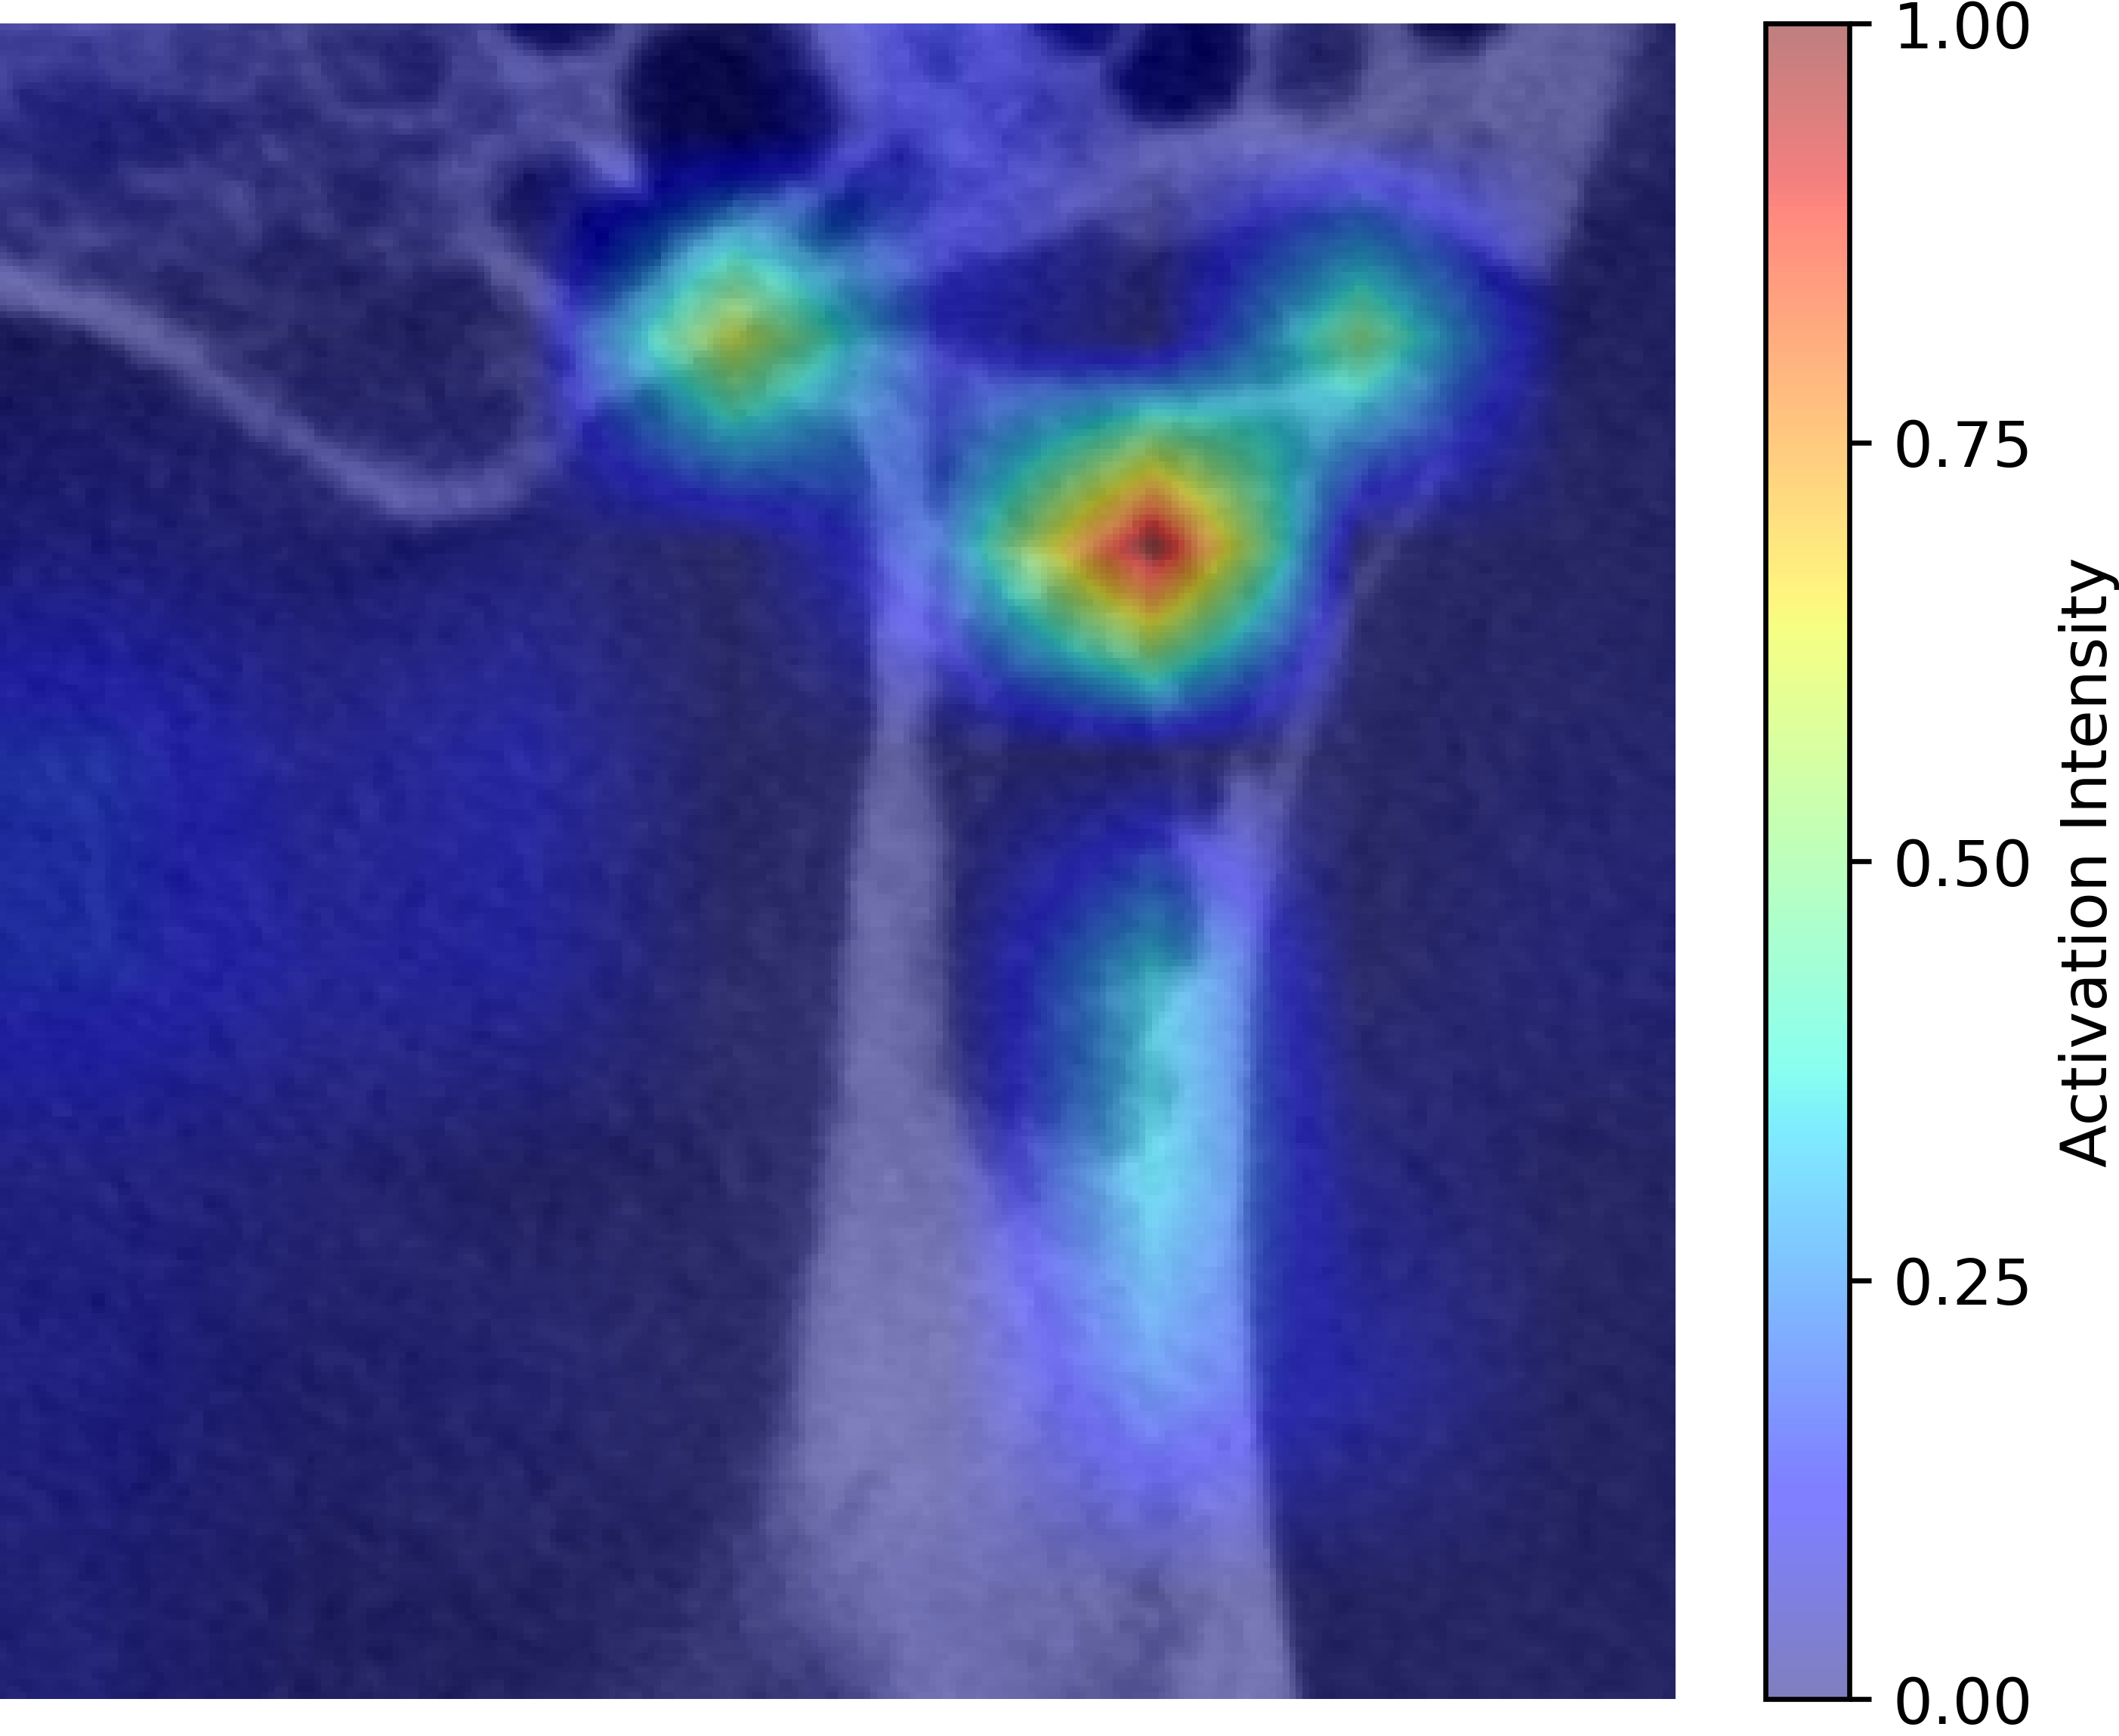
\includegraphics[width=\cellw]{figures/erosion_overlayed_130.png} \\[6pt]
%     \textbf{(D)} & \textbf{(E)} & \textbf{(F)} \\[-2pt]
%     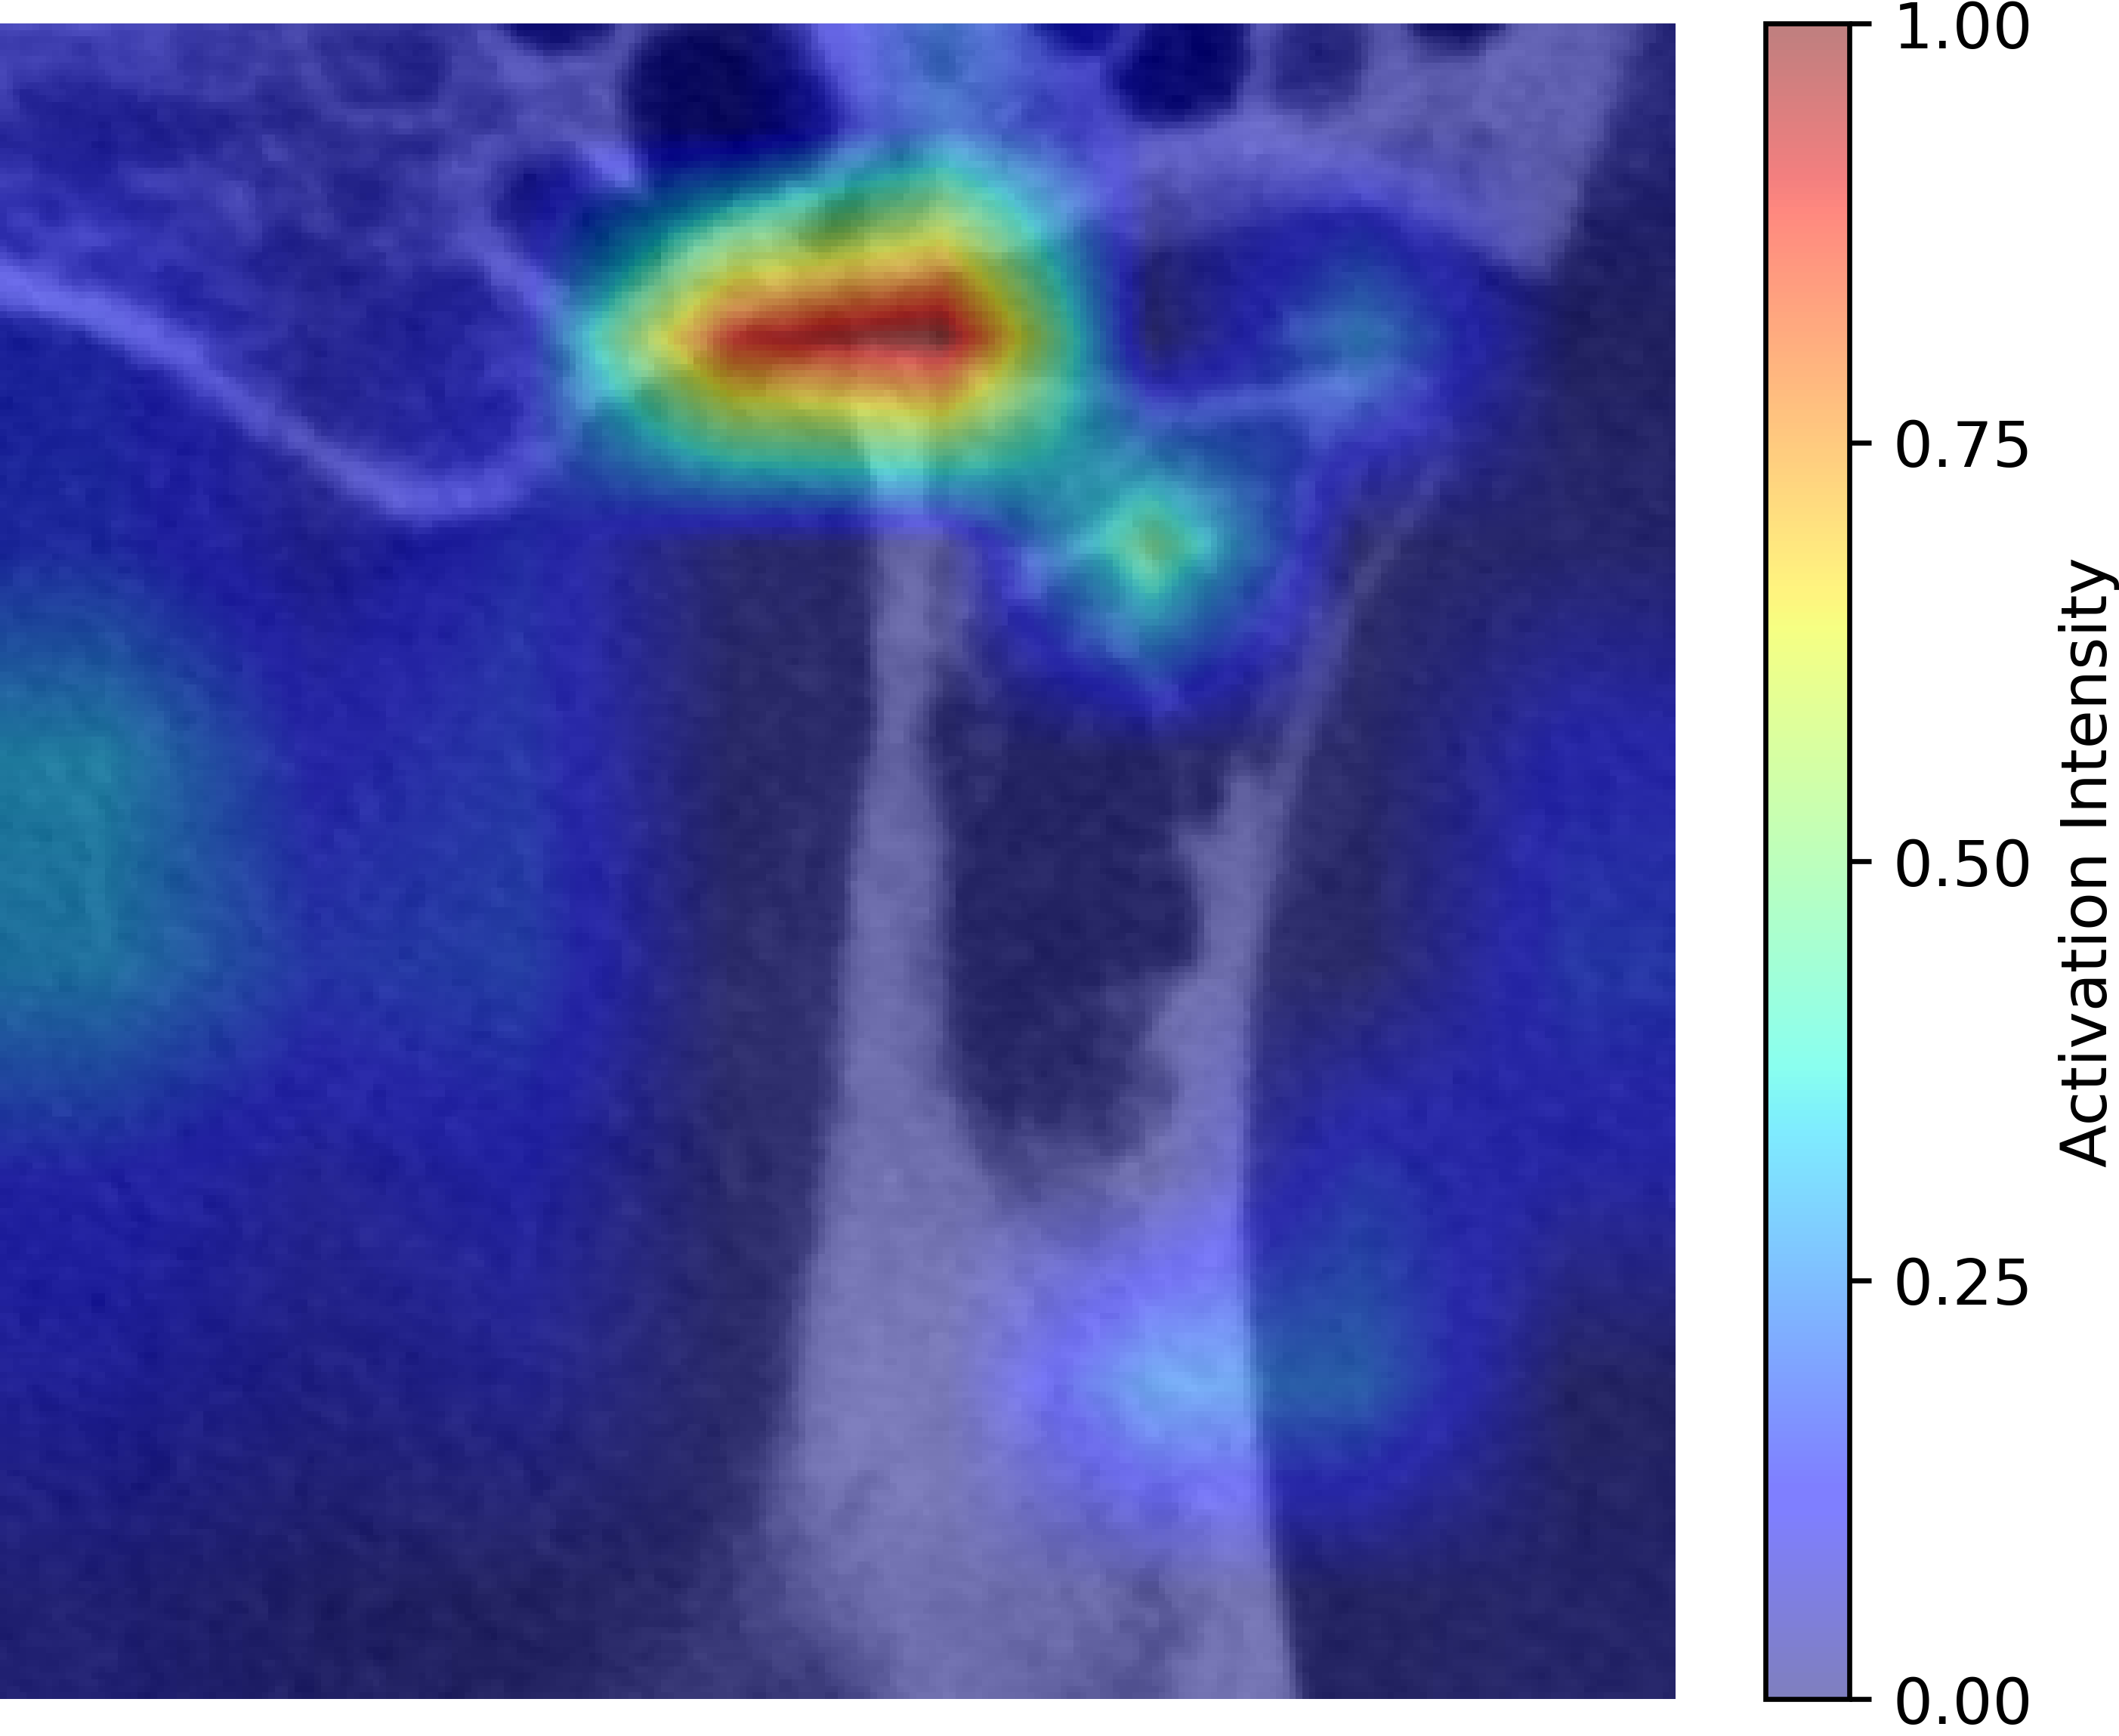
\includegraphics[width=\cellw]{figures/genSclerosis_overlayed_130.png} &
%     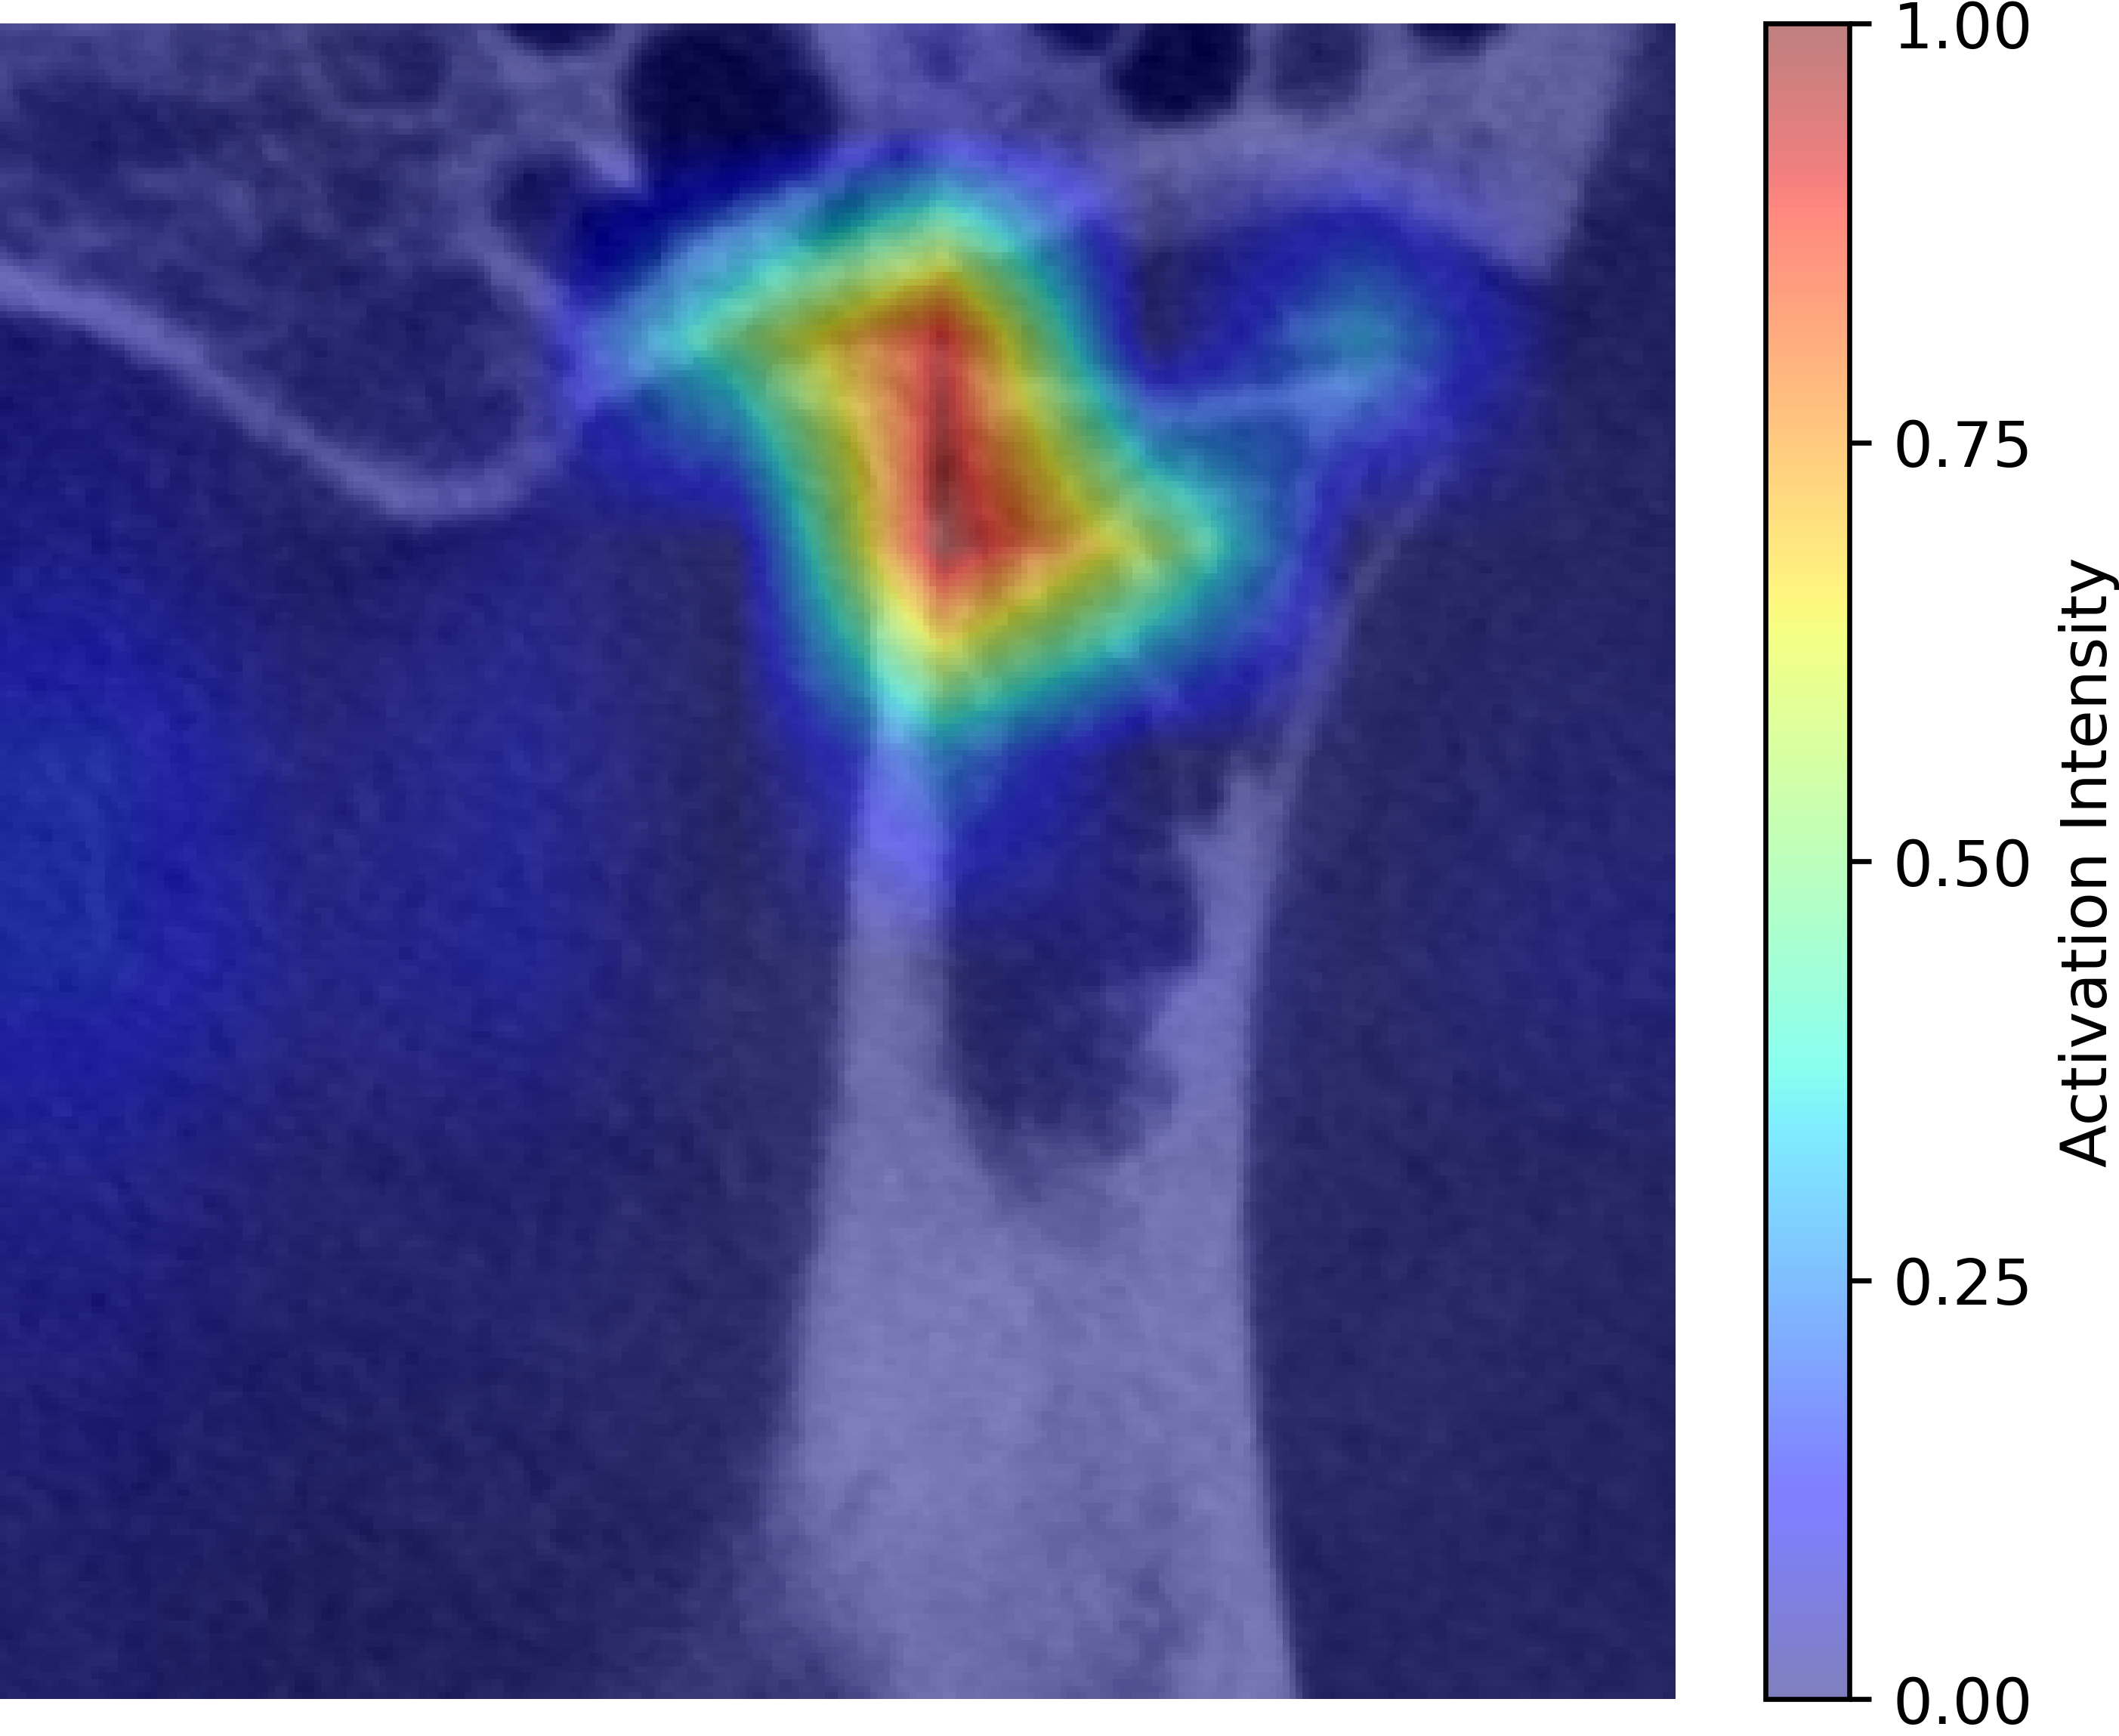
\includegraphics[width=\cellw]{figures/osteophyte_overlayed_130.png} &
%     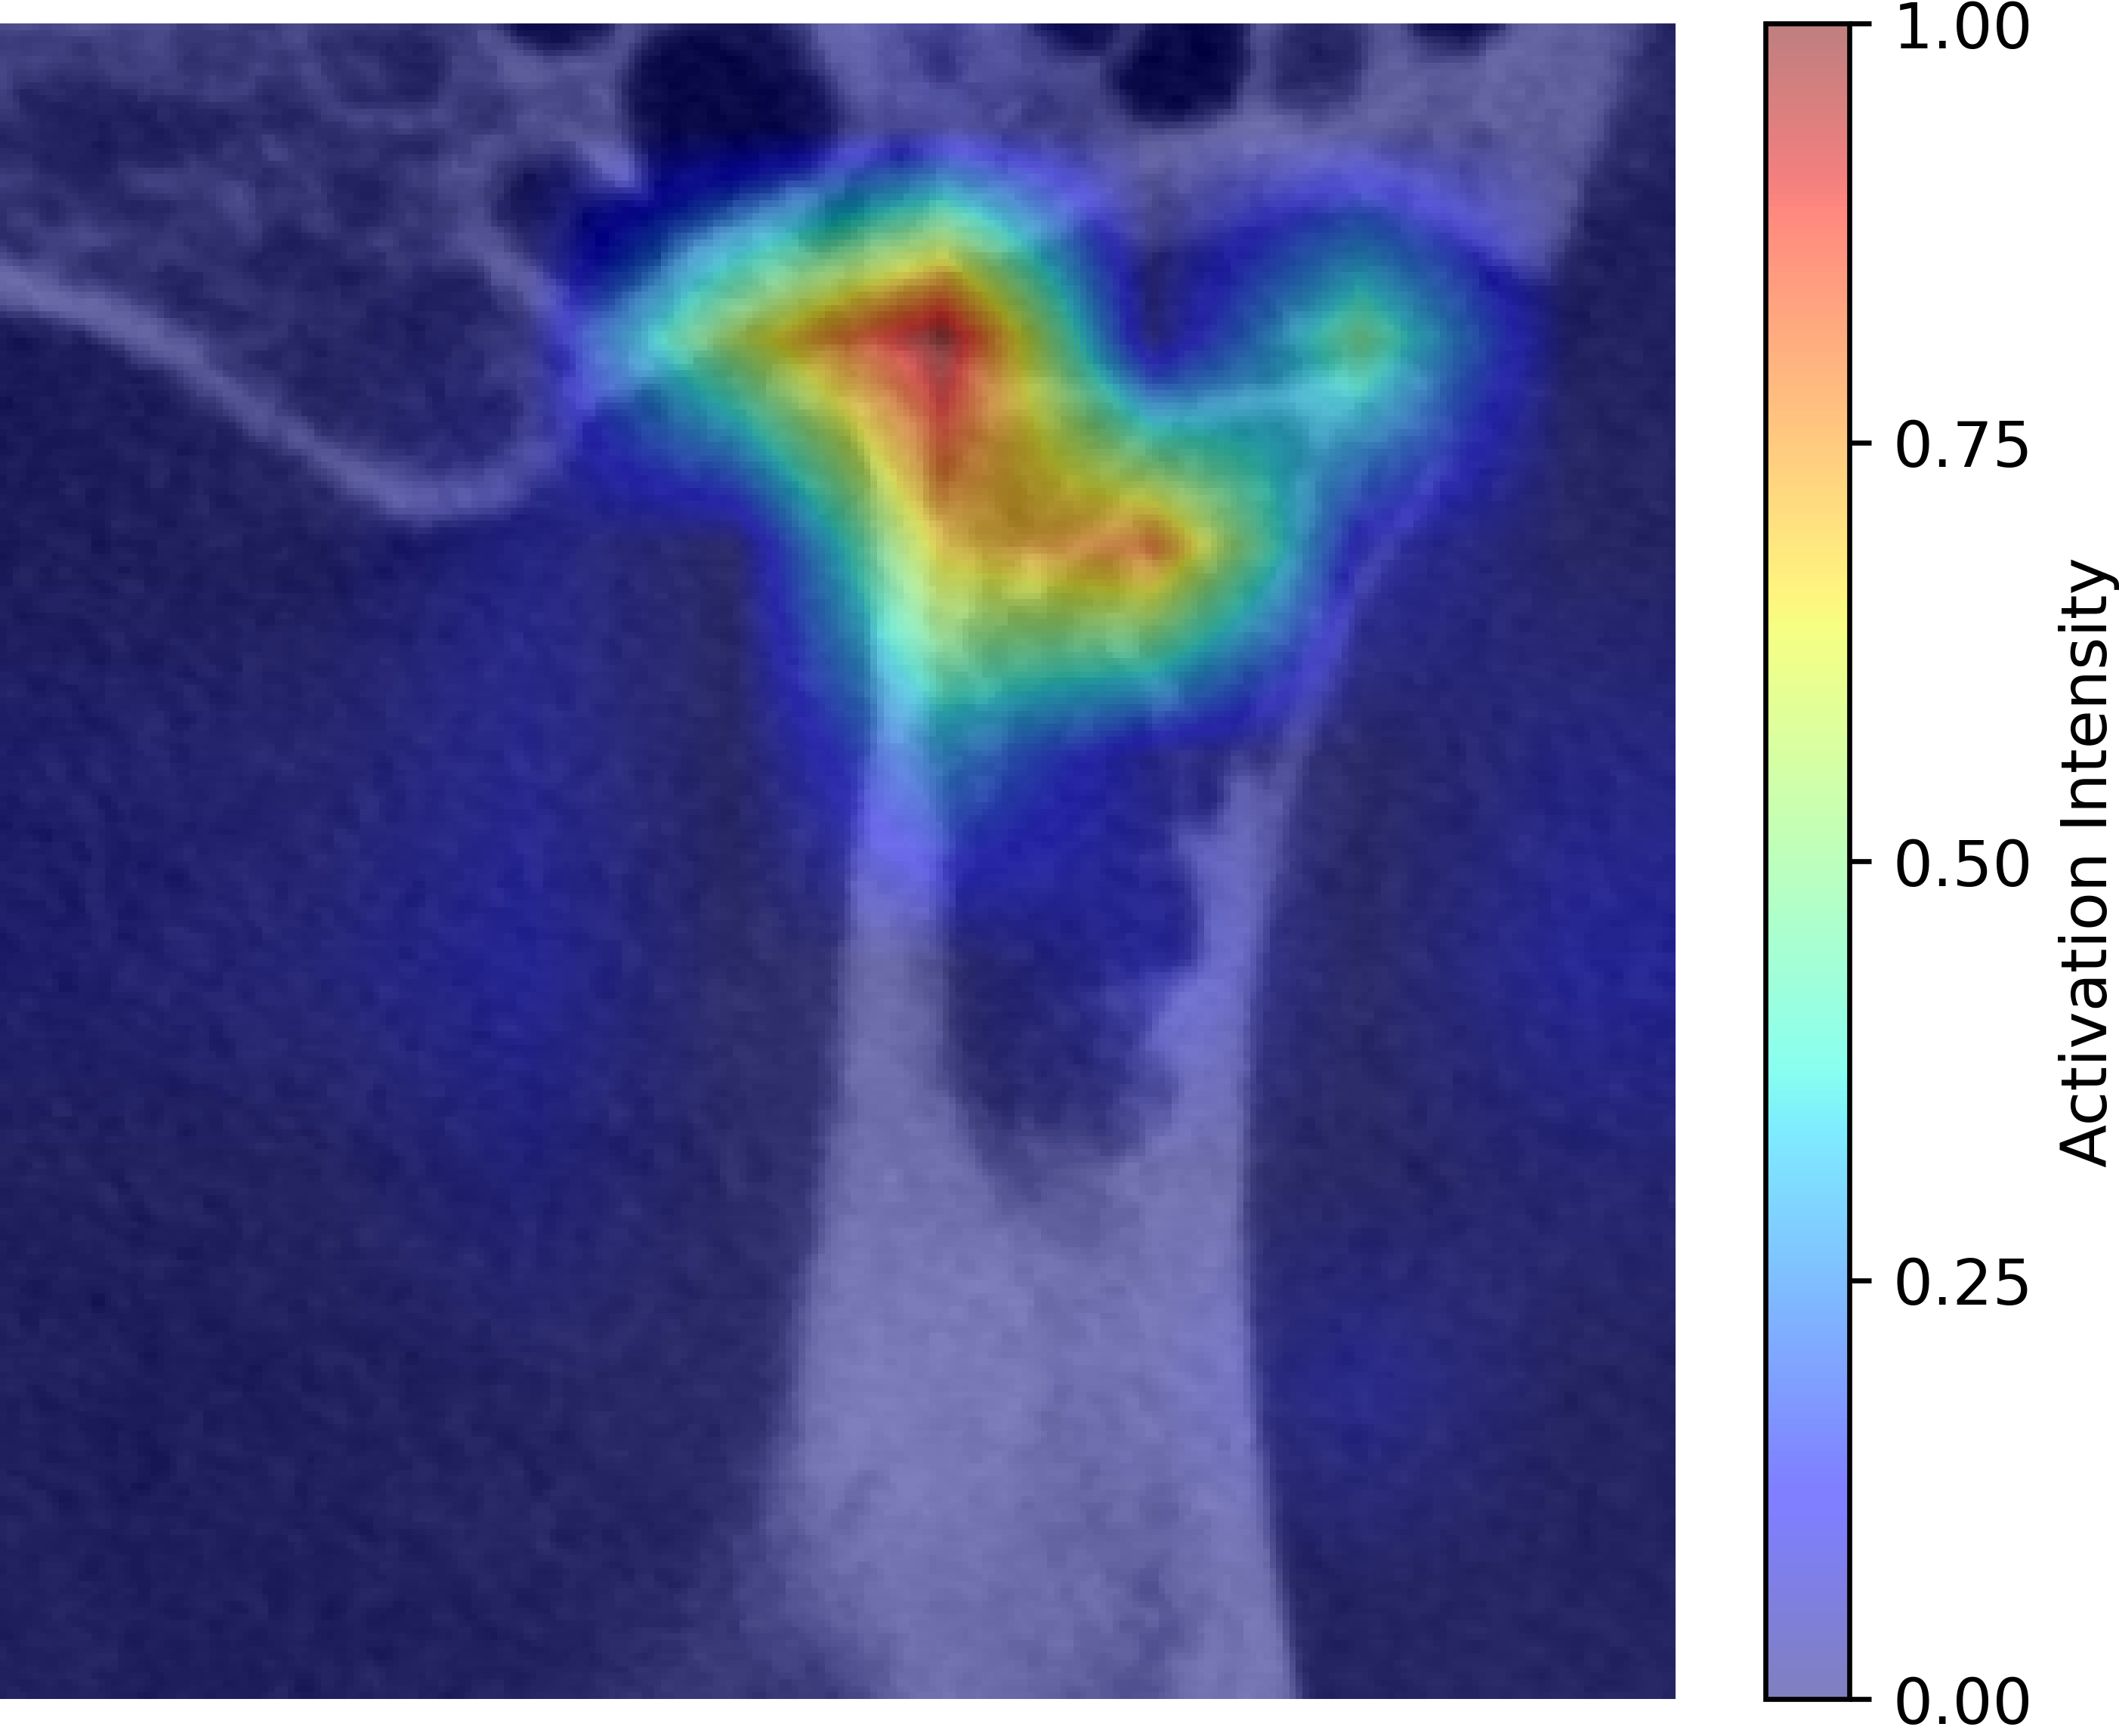
\includegraphics[width=\cellw]{figures/subCyst_overlayed_130.png} \\
%   \end{tabular}
%   \caption{GradCAM visualisation for ConvNeXt. (A)~Sagittal slice
%   (original), and GradCAM overlays for true-positive predictions of
%   (B)~Osteoarthritis, (C)~Condylar erosion, (D)~Generalised sclerosis,
%   (E)~Osteophyte, and (F)~Subchondral cyst.}
%   \label{fig:gradcam}
% \end{figure}

% \begin{figure}[htbp]
%   \centering
%   \includegraphics[width=\textwidth]{figures/roc_auc_bar_chart.png}
%   \caption{AUC-ROC across five tasks for all 20 backbone architectures.}
%   \label{fig:model_comparison2D}
% \end{figure}

% \begin{figure}[htbp]
%   \centering
%   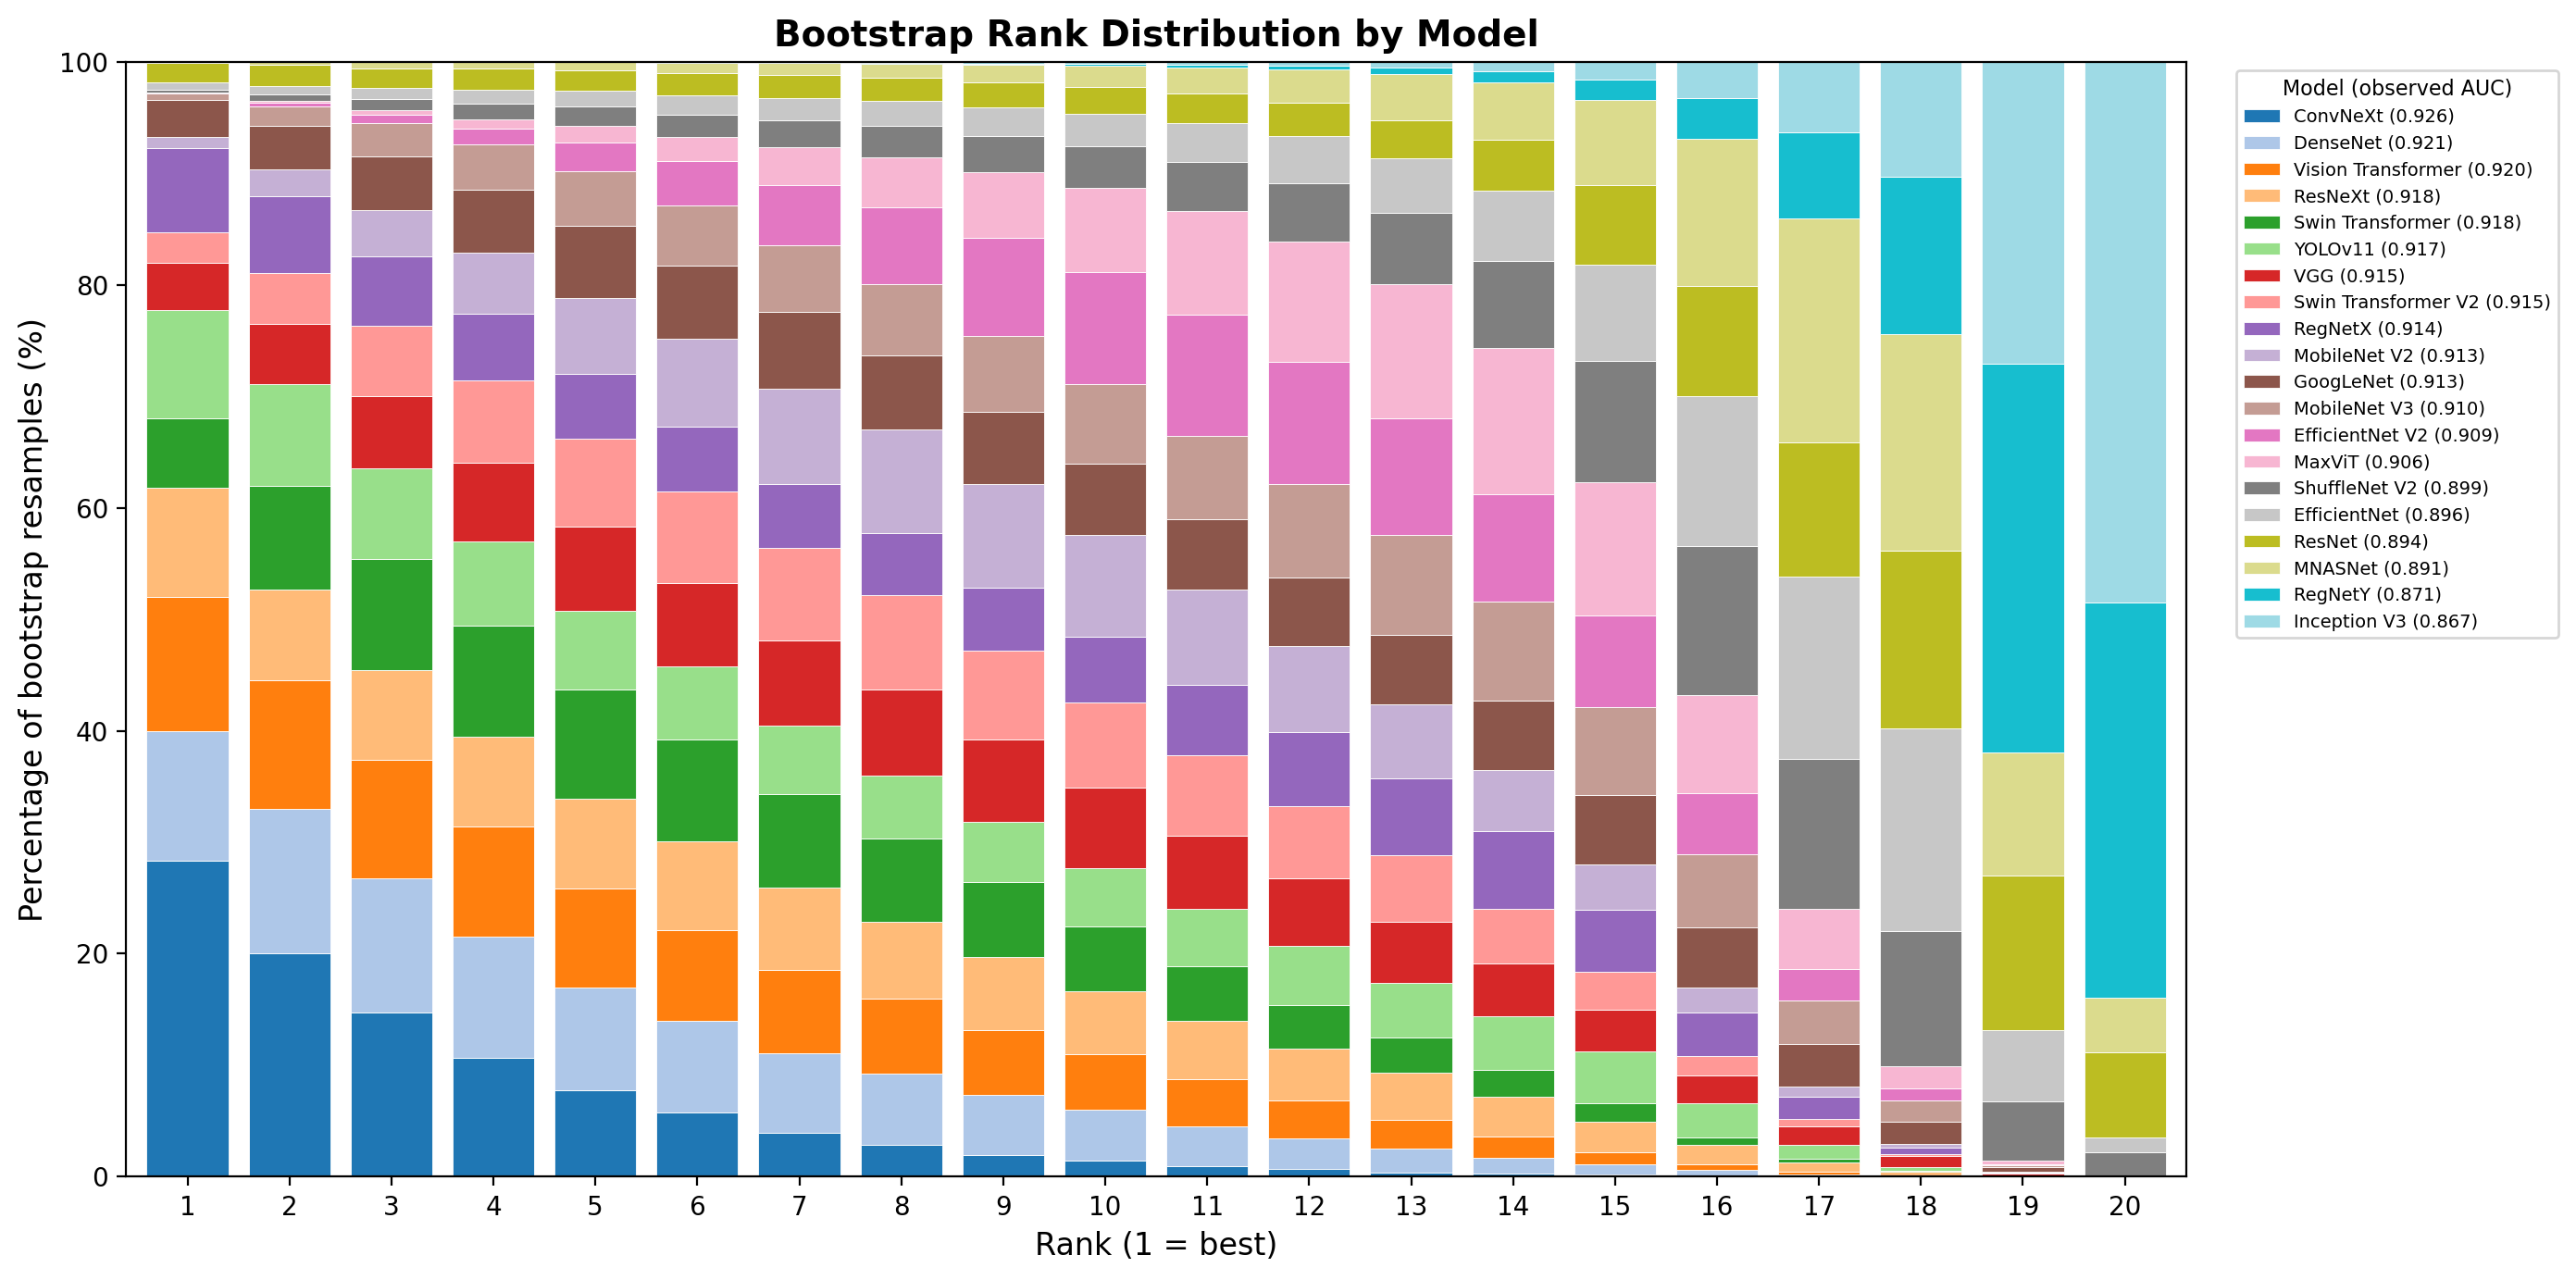
\includegraphics[width=0.8\textwidth]{figures/bootstrap_dist.png}
%   \caption{Bootstrap rank distribution across 10{,}000 resamples for all
%   20 architectures, sorted by observed mean AUC-ROC. Stacked bars indicate the
%   proportion of resamples in which each architecture achieved a given
%   rank. Substantial rank overlap among the top 10 models indicates that
%   observed performance differences are not robust to sampling
%   variability.}
%   \label{fig:bootstrap_rank}
% \end{figure}


%% ===================================================================
%% REFERENCES
%% ===================================================================
\newpage
\bibliographystyle{elsarticle-num}
\bibliography{references}

\end{document}